%----------------------------------------------------------------------------------------
%   Доорх хэсгийг өөрчлөх шаардлагагүй
%----------------------------------------------------------------------------------------
%!TEX TS-program = xelatex
%!TEX encoding = UTF-8 Unicode
\documentclass[12pt,A4]{report}

\usepackage{fontspec,xltxtra,xunicode}
\setmainfont[Ligatures=TeX]{Times New Roman}
\setsansfont{Arial}
\setmonofont[Scale=0.85]{DejaVu Sans Mono}

% \usepackage[utf8x]{inputenc}
% \usepackage[mongolian]{babel}
%\usepackage{natbib}
\usepackage{geometry}
%\usepackage{fancyheadings} fancyheadings is obsolete: replaced by fancyhdr. JL
\usepackage{fancyhdr}
\usepackage{float}
\usepackage{afterpage}
\usepackage{graphicx}
\usepackage{amsmath,amssymb,amsbsy}
\usepackage{dcolumn,array}
\usepackage{tocloft}
\usepackage{dics}
\renewcommand{\tablename}{Хүснэгт}
\renewcommand{\bibname}{Ном зүй}
\setlength{\emergencystretch}{3em}
\setlength{\headheight}{15pt}
\usepackage{array}
\usepackage{longtable}
\usepackage{nomencl}
\usepackage{upgreek}
\newcommand{\argmin}{\arg\!\min}
\usepackage{mathtools}
\usepackage[hidelinks]{hyperref}

\usepackage{algorithm}
\usepackage{algpseudocode}

\usepackage{listings}
\DeclarePairedDelimiter\abs{\lvert}{\rvert}%
\makeatletter
\usepackage{caption}
\captionsetup[table]{belowskip=0.5pt}
\usepackage{subfiles}

\usepackage{listings}
\renewcommand{\lstlistingname}{Код}
\renewcommand{\lstlistlistingname}{\lstlistingname ын жагсаалт}

\usepackage{color}
\definecolor{codegreen}{rgb}{0,0.6,0}
\definecolor{codegray}{rgb}{0.5,0.5,0.5}
\definecolor{codepurple}{rgb}{0.58,0,0.82}
\definecolor{backcolour}{rgb}{0.99,0.99,0.99}
 
\lstdefinestyle{mystyle}{
    basicstyle=\ttfamily\small,
    backgroundcolor=\color{backcolour},   
    commentstyle=\color{codegreen},
    keywordstyle=\color{magenta},
    numberstyle=\tiny\color{codegray},
    stringstyle=\color{codepurple},
    %basicstyle=\footnotesize,
    breakatwhitespace=false,         
    breaklines=true,                 
    captionpos=b,                    
    keepspaces=false,                 
    numbers=left,                    
    numbersep=10pt,                  
    showspaces=false,                
    showstringspaces=true,
    showtabs=false,                  
    tabsize=2
}
 
\lstset{style=mystyle, label=DescriptiveLabel} 

\let\oldabs\abs
\def\abs{\@ifstar{\oldabs}{\oldabs*}}
\makenomenclature
\begin{document}


%----------------------------------------------------------------------------------------
%   Өөрийн мэдээллээ оруулах хэсэг
%----------------------------------------------------------------------------------------

% Дипломийн ажлын сэдэв
\title{Спортын шинжилгээнд хүний байрлалын тооцооллыг ашиглах нь}
% Дипломын ажлын англи нэр
\titleEng{Using human pose estimation in sport analytics}
% Өөрийн овог нэрийг бүтнээр нь бичнэ
\author{Баатар овогтой Түвшинжаргал}
% Өөрийн овгийн эхний үсэг нэрээ бичнэ
\authorShort{Б.Түвшинжаргал}
% Удирдагчийн зэрэг цол овгийн эхний үсэг нэр
\supervisor{Дэд Профессор Б.Наранчимэг}

% СиСи дугаар
\sisiId{22B1NUM6969}
% Их сургуулийн нэр
\university{МОНГОЛ УЛСЫН ИХ СУРГУУЛЬ}
% Бүрэлдэхүүн сургуулийн нэр
\faculty{МЭДЭЭЛЛИЙН ТЕХНОЛОГИ, ЭЛЕКТРОНИКИЙН СУРГУУЛЬ}
% Тэнхимийн нэр
\department{МЭДЭЭЛЭЛ, КОМПЬЮТЕРЫН УХААНЫ ТЭНХИМ}
% Зэргийн нэр
\degreeName{Бакалаврын судалгааны ажил}
% Суралцаж буй хөтөлбөрийн нэр
\programeName{Мэдээллийн систем}
% Хэвлэгдсэн газар
\cityName{Улаанбаатар}
% Хэвлэгдсэн огноо
\gradyear{2026 оны 11 дүгээр сар}


%----------------------------------------------------------------------------------------
%   Доорх хэсгийг өөрчлөх шаардлагагүй
%----------------------------------------------------------------------------------------
%----------------------Нүүр хуудастай хамаатай зүйлс----------------------------
\pagenumbering{roman}
\makefrontpage
\maketitle

\doublespace

% Decleration
\begin{huge}
\textbf{Зохиогчийн баталгаа}
\end{huge} \\ \ \\ 
\doublespace
Миний бие \@author \ "\@title" \ сэдэвтэй судалгааны ажлыг гүйцэтгэсэн болохыг зарлаж дараах зүйлсийг баталж байна:
\begin{itemize}
\item Ажил нь бүхэлдээ Монгол Улсын Их Сургуульд дээд боловсролын зэрэг горилохоор дэвшүүлсэн болно.
\item Энэ ажлын аль нэг хэсгийг эсвэл бүхлээр нь ямар нэг их, дээд сургуулийн зэрэг горилохоор оруулж байгаагүй болно.
\item Бусдын хийсэн ажлаас хуулбарлаагүй, эшлэл, зүүлтийг зохистой хийсэн болно.
\item Ажлыг зохиогч би хийсэн ба миний хийсэн ажил, бусдын дэмжлэгийг дипломын ажилд тодорхой тусгасан болно. 
\item Ажилд тусалсан бүх эх сурвалжид талархаж байна. 
\end{itemize} 
\ 

Гарын үсэг: \underline{\hspace{5cm}} 

Огноо: 	\ \ \underline{\hspace{3cm}}

% Гарчгийг автоматаар оруулна
\setcounter{tocdepth}{1}
% Гарчгийг нэг хуудсанд багтаахын тулд 1.24 мөрийн зайтай (dics.sty нь энд doublespace тавьдаг)
\begingroup
\let\doublespace\oneandhalfspace
\tableofcontents
\endgroup
\doublespace

% Зургийн жагсаалтыг автоматаар оруулна
\listoffigures

% Хүснэгтийн жагсаалтыг автоматаар оруулна
\listoftables

% Кодын жагсаалтыг автоматаар оруулна
\lstlistoflistings
% Жагсаалтын толгой гарчиг дараагийн хуудсуудад үлдэхгүй байх
\markboth{}{}

% Түлхүүр үгийн тайлбар glossary.tex файлд бичигдсэн
%----------------------------------------------------------------------------------------
%   Түлхүүр үгийн тайлбар
%   Шинэ үг нэмэхдээ жагсаалтад \item нэмнэ. Цагаан толгойн дарааллыг хадгална уу.
%----------------------------------------------------------------------------------------
\newpage
\begingroup
\renewcommand{\headrulewidth}{0pt}
\markboth{}{}
\begin{center}
\textbf{\large ТҮЛХҮҮР ҮГИЙН ТАЙЛБАР}
\end{center}

\singlespace

\noindent\textbf{Товчилсон үг}

\begin{description}
\item[2D, 3D] Two-, Three-Dimensional --- Хоёр хэмжээст, гурван хэмжээст
\item[API] Application Programming Interface --- Програмууд хоорондоо хүсэлт илгээж харилцах интерфейс
\item[COCO] Common Objects in Context --- Хүний гол цэгийн тэмдэглэгээтэй, өргөн хэрэглэгддэг зургийн өгөгдлийн сан
\item[CPU] Central Processing Unit --- Компьютерын төв процессор
\item[CSV] Comma-Separated Values --- Таслалаар тусгаарласан хүснэгтэн өгөгдлийн файлын формат
\item[CUDA] Compute Unified Device Architecture --- NVIDIA-ийн GPU дээр ерөнхий тооцоолол хийх платформ
\item[CV] Coefficient of Variation --- Хэлбэлзлийн коэффициент
\item[DTW] Dynamic Time Warping --- Динамик цагийн хазайлт; хурд нь ялгаатай хоёр цувааг харьцуулах арга
\item[GPU] Graphics Processing Unit --- График процессор (видео карт)
\item[HPE] Human Pose Estimation --- Хүний байрлал тодорхойлох
\item[HRNet] High-Resolution Network --- Өндөр нягтаршилтай дүрслэлд суурилсан HPE загвар
\item[JSON] JavaScript Object Notation --- Бүтэцтэй өгөгдөл хадгалах текст формат
\item[LSP] Leeds Sports Pose --- Спортын байрлалын өгөгдлийн сан
\item[MAE] Mean Absolute Error --- Дундаж абсолют алдаа
\item[MP4] MPEG-4 Part 14 --- Видео файлын формат
\item[MPII] MPII Human Pose --- Хүний байрлалын өгөгдлийн сан
\item[NMS] Non-Maximum Suppression --- Давхацсан илрүүлэлтүүдээс хамгийн өндөр итгэлцэлтэйг үлдээх алхам
\item[ONNX] Open Neural Network Exchange --- Нейрон сүлжээний загварыг өөр орчинд шилжүүлэх нээлттэй формат
\item[PAF] Part Affinity Fields --- Хэсгийн холбоосын талбар; OpenPose-д гол цэгүүдийг хүн тус бүрээр холбоход ашиглана
\item[PCK] Percentage of Correct Keypoints --- Зөв илэрсэн гол цэгийн хувь
\item[RTMPose] Real-Time Multi-person Pose Estimation --- Бодит хугацааны олон хүний байрлал тодорхойлох загвар
\item[SHA-256] Secure Hash Algorithm (256-bit) --- Файл ижил эсэхийг шалгах хэш функц
\item[SimCC] Simple Coordinate Classification --- RTMPose-ийн гол цэгийн x, y координатыг тэнхлэг тус бүрээр ангилж тодорхойлох гаралт
\item[ViT] Vision Transformer --- Зургийн трансформер; ViTPose загварын суурь архитектур
\item[WASM] WebAssembly --- Вэб хөтөч дотор CPU дээр хурдан ажиллах кодын формат
\item[WebGL] Web Graphics Library --- Вэб хөтөчөөс GPU ашиглан график зурах технологи
\item[WebGPU]Вэб хөтөчөөс GPU-ийн тооцооллыг шууд ашиглах шинэ технологи
\item[YOLO] You Only Look Once --- Объект илрүүлэлтийг нэг алхамд гүйцэтгэдэг загваруудын гэр бүл
\end{description}

\noindent\textbf{Нэр томьёо}

\begin{description}
\item[Араг яс (skeleton)] Гол цэгүүдийг хооронд нь шугамаар холбосон хүний биеийн энгийн дүрслэл
\item[Гол цэг (keypoint)] Хамар, мөр, тохой, өвдөг зэрэг хүний биеийн анатомийн тодорхой цэг
\item[Гулсах цонх (sliding window)] Хугацааны цувааны тодорхой урттай хэсгийг шилжүүлэн тооцоолол хийх арга
\item[Дээрээс доош (top-down)] Эхлээд хүн бүрийг хүрээгээр илрүүлж, дараа нь хүрээ тус бүрт гол цэгийг тодорхойлдог HPE арга
\item[Доороос дээш (bottom-up)] Эхлээд бүх гол цэгийг илрүүлж, дараа нь хүн тус бүрээр бүлэглэдэг HPE арга
\item[Жинхэнэ утга (ground truth)] Гараар тэмдэглэсэн, зөв гэж тооцогдох жишиг өгөгдөл
\item[Консенсус (consensus)] Бусад загваруудын гаргасан байрлалын медиан; жинхэнэ утга байхгүй үед жишиг болгон ашиглана
\item[Корреляц (correlation)] Хоёр цуваа хэр зэрэг хамт өөрчлөгдөж байгааг $-1$-ээс 1 хүртэлх утгаар илэрхийлэх хэмжүүр
\item[Сервер (server)] Хэрэглэгчийн хүсэлтээр тооцоолол гүйцэтгэж үр дүнг буцаадаг алсын компьютер; энэ ажилд видеоны гол цэгийг тодорхойлно
\item[Синхрончлол (synchronization)] Хоёр болон түүнээс дээш хүний хөдөлгөөн хэлбэр, хэмнэл, цаг хугацааны хувьд хэр нийцэж буй байдал
\item[Тооцооллын backend (execution provider)] Загварын тооцооллыг гүйцэтгэх технологи (WebGPU, WASM, CUDA гэх мэт)
\item[Үений өнцөг (joint angle)] Гурван гол цэгээр тодорхойлогдох үений нугаралтын өнцөг, жишээлбэл тохойн өнцөг
\item[Хөндлөн корреляц (cross-correlation)] Нэг цувааг цаг хугацааны дагуу шилжүүлэн нөгөөтэй нь харьцуулж, цагийн хоцрогдлыг олох арга
\item[Хяналттай өгөгдөл (synthetic data)] Хоцрогдол, зай зэрэг ялгааг судлаач өөрөө тогтоож үүсгэсэн туршилтын өгөгдөл
\item[Цагийн хоцрогдол (lag)] Нэг хүний хөдөлгөөн нөгөөгөөсөө хэдэн кадр эсвэл секундээр хоцорч байгааг илэрхийлэх утга
\item[Чичиргээ (jitter)] Хүн хөдөлгөөнгүй байсан ч дараалсан кадруудад гол цэгийн байрлал санамсаргүй үсрэх үзэгдэл
\item[Шуугиан тэгшитгэх (smoothing)] Хөрш кадруудын утгыг ашиглан чичиргээг багасгаж, хөдөлгөөний муруйг гөлгөр болгох алхам
\end{description}

\doublespace
\newpage
\endgroup


% This puts the word "Page" right justified above everything else.
\newpage
%% \addtocontents{lof}{Зураг~\hfill Хуудас \par}
\newpage
%% \addtocontents{lot}{Хүснэгт~\hfill Хуудас \par}

\renewcommand{\cftlabel}{Зураг}


\doublespace
\pagenumbering{arabic}


% Удиртгал abstract.tex файлд бичигдсэн
\begin{abstract}
Хоёр болон түүнээс дээш хүний хамтын хөдөлгөөний синхрончлол нь хос болон бүлгийн бүжиг, спортын хос болон багийн төрөл, дасгалжуулагч ба тамирчны дасгал, сэргээн засах эмчилгээ зэрэг салбарт гүйцэтгэлийн чанарыг тодорхойлох чухал үзүүлэлт юм. Уламжлалт байдлаар синхрончлолыг дасгалжуулагч, шүүгч эсвэл мэргэжилтэн нүдээр ажиглан үнэлдэг бөгөөд энэ үнэлгээ нь хүний субъектив дүгнэлтээс ихээхэн хамаардаг, тоон хэмжүүргүй, давтагдах боломж муутай байдаг. Мөн хөдөлгөөн бүртгэх (motion capture) тоног төхөөрөмж ашиглах нь өндөр өртөгтэй, тусгай мэдрэгч зүүх шаардлагатай тул өдөр тутмын хэрэглээнд тохиромжгүй. Иймд хүний байрлал тодорхойлох (Human Pose Estimation, HPE) технологи ашиглан хүмүүсийн биеийн гол цэгүүдийг тодорхойлж, тэдгээрийн хөдөлгөөний ижил төстэй байдал болон синхрончлолын түвшнийг тоон утгаар үнэлэх арга боловсруулах нь онолын болон практик ач холбогдолтой асуудал болж байна.

\medskip\noindent\textbf{Судалгааны ажлын зорилго}\par
Энэхүү судалгааны ажлын зорилго нь хоёр болон түүнээс дээш хүний хөдөлгөөний өгөгдөл өгөгдсөн үед HPE загвар ашиглан тэдгээрийн биеийн гол цэгүүдийг тодорхойлж, гол цэгүүдийн байрлал болон үений өнцөгт үндэслэн хүмүүсийн хөдөлгөөний ижил төстэй байдал болон синхрончлолын түвшнийг тоон хэмжүүрээр тооцоолох алгоритм боловсруулах явдал юм. Хэрэгжүүлэлтийг хийхдээ үндсэн тохиолдолд хоёр хүний хөдөлгөөнийг харьцуулах бөгөөд хүний тоо нэмэгдэхэд хүмүүсийг хос хосоор нь харьцуулж, дундажлан бүлгийн синхрончлолыг үнэлнэ. Мөн боловсруулсан алгоритмын үр дүнг синхрончлолын түвшин урьдчилан мэдэгдэж буй туршилтын өгөгдөл дээр шалгаж нарийвчлал болон гүйцэтгэлийг туршилтаар үнэлэх, практикт ашиглах боломж болон хязгаарлалтыг тодорхойлоход оршино.

\medskip\noindent\textbf{Судалгааны ажлын зорилтууд}\par
Тус зорилгыг хэрэгжүүлэхийн тулд дараах зорилтуудыг дэвшүүлэв. Үүнд:

\begin{enumerate}
\def\labelenumi{\arabic{enumi}.}
\item
  Хүний байрлал тодорхойлох технологийн онол, арга зүй болон хөдөлгөөний синхрончлолыг үнэлэх одоо ашиглагдаж буй аргачлалуудыг судлах
\item
  Видео бичлэгээс хүний биеийн гол цэгүүдийг илрүүлэх HPE загваруудыг (OpenPose, MediaPipe, YOLO-Pose, HRNet гэх мэт) харьцуулан судалж, шаардлагатай гол цэгийн тоо болон гүйцэтгэлд үндэслэн туршилтад ашиглах загварыг сонгох
\item
  Хоёр болон түүнээс дээш хүний хөдөлгөөнийг агуулсан туршилтын өгөгдлийг бэлтгэж, бичлэгт тавигдах шаардлагыг тодорхойлох
\item
  Илэрсэн гол цэгүүдийн өгөгдлийн дутуу цэгийг нөхөх, шуугиан арилгах урьдчилсан боловсруулалтын алгоритм боловсруулах
\item
  Гол цэгүүдийн байрлал, үений өнцөг болон хугацааны цуваанд үндэслэн хүмүүсийн хөдөлгөөний ижил төстэй байдал болон бүлгийн синхрончлолын түвшнийг тооцоолох алгоритм боловсруулах
\item
  Боловсруулсан алгоритмыг туршиж, синхрончлолын үнэлгээний үр дүнг синхрончлолын түвшин урьдчилан мэдэгдэж буй бичлэгүүд дээр шалгаж нарийвчлал, боловсруулалтын хурд болон найдвартай байдлыг статистик хэмжүүрээр үнэлэх
\item
  Видео бичлэгийн нягтаршил, кадрын давтамж зэрэг оролтын өгөгдлийн шинж чанар алгоритмын үр дүнд хэрхэн нөлөөлөхийг туршилтаар судалж, аргын боломж болон хязгаарлалтыг тодорхойлох
\end{enumerate}

\medskip\noindent\textbf{Судалгааны үр дүн}\par
Таван HPE загварыг харьцуулж RTMPose-m загварыг сонгон, үений өнцгийн зөрүү, корреляц, хөндлөн корреляцаар олсон цагийн хоцрогдлыг нэгтгэсэн синхрончлолын алгоритмыг вэб хөтөч болон сервер дээр ажилладаг систем болгон хэрэгжүүлэв. Нэг хүний бичлэгээс FFmpeg-ээр үүсгэсэн 32 хяналттай бичлэг дээр алгоритм 0--1 секундийн бүх хоцрогдлыг 0 мс алдаатай олж, синхрон (99.8), хоцрогдолтой (54.3--97.1) болон өөр хөдөлгөөнтэй (45.4--62.0) бичлэгүүдийг ялгаж, толин тусгал хөдөлгөөнийг таньж, 3 ба 4 хүнтэй бичлэгт хоцорсон хүнийг зөв илрүүлэв. Хүний хэмжээ 50\%, нягтаршил 360p, кадрын давтамж 10 кадр/с хүртэл буурахад үр дүн бараг өөрчлөгдөөгүй бол хүний өндөр ойролцоогоор 140 пикселээс бага үед хүний тоог автоматаар тоолох алхам алдаа гаргасан нь аргын гол хязгаарлалт болов.
\end{abstract}


%----------------------------------------------------------------------------------------
%   Үндсэн хэсэг
%----------------------------------------------------------------------------------------
% Толгой гарчиг: зүүн талд дэд бүлэг, баруун талд бүлэг. Урт гарчиг давхцахгүйн тулд
% тус бүрийг өөрийн өргөнд багтааж, шаардлагатай бол хоёр мөрөнд хуваана.
\fancyhead[L]{\fancyplain{}{\parbox[b]{0.50\textwidth}{\raggedright\slshape\rightmark}}}
\fancyhead[R]{\fancyplain{}{\parbox[b]{0.46\textwidth}{\raggedleft\slshape\leftmark}}}

% Урт гарчгийн оронд толгой гарчигт богино нэр харуулах: \headshort{Богино нэр} гэж
% \chapter эсвэл \section-ий өмнө бичнэ. Гарчигийн жагсаалтад бүтэн нэр хэвээр үлдэнэ.
\makeatletter
\let\@headshort\@empty
\newcommand{\headshort}[1]{\gdef\@headshort{#1}}
\renewcommand{\sectionmark}[1]{\markright{\MakeUppercase{\ifnum\c@secnumdepth>\z@\thesection.\ \fi\ifx\@headshort\@empty #1\else\@headshort\fi}}\global\let\@headshort\@empty}
\renewcommand{\chaptermark}[1]{\markboth{\MakeUppercase{\ifnum\c@secnumdepth>\m@ne\@chapapp\ \thechapter.\ \fi\ifx\@headshort\@empty #1\else\@headshort\fi}}{}\global\let\@headshort\@empty}
\makeatother

\chapter{Ерөнхий хэсэг}
\section{Сэдэв сонгосон үндэслэл}

Гүн сургалтад суурилсан хүний байрлал тодорхойлох технологийн хөгжлөөр энгийн камерын бичлэгээс хүний хөдөлгөөнийг үнэтэй тоног төхөөрөмж, биед зүүдэг мэдрэгчгүйгээр тоон өгөгдөл болгох боломж бүрдсэн. Харин хос бүжиг, спорт, сэргээн засах эмчилгээ зэрэгт олон хүний хөдөлгөөний синхрончлолыг одоог хүртэл мэргэжилтэн нүдээр, субъектив байдлаар үнэлсээр байна. Иймд синхрончлолыг автоматаар, тоон утгаар үнэлэх системийг судалгааны сэдвээ болгон сонгосон.

Хүний байрлал тодорхойлох чиглэлд OpenPose, HRNet, MediaPipe Pose, YOLO-Pose зэрэг олон загвар боловсруулагдсан бөгөөд хөдөлгөөний ижил төстэй байдлыг косинус төстэй байдал, Евклидийн зай, динамик цагийн хазайлт (Dynamic Time Warping, DTW) \cite{sakoe1978}, хөндлөн корреляц зэрэг аргаар харьцуулдаг. Гэвч эдгээр судалгааны ихэнх нь хүнийг лавлах хөдөлгөөнтэй харьцуулдаг бөгөөд зэрэг хөдөлж буй олон хүний синхрончлол, мөн бичлэгийн нягтаршил, кадрын давтамжийн нөлөөг судалсан ажил цөөн байна.

\section{Системийн хэрэгцээ шаардлага}

Систем нь дараах шаардлагуудыг хангах ёстой. Үүнд:

\begin{itemize}
\item
  Хоёр болон түүнээс дээш хүнтэй видеоноос хүн бүрийн гол цэгийг илрүүлж, тухайн хүнд хамааруулах
\item
  Биеийн хэмжээ, камерын зайнаас үл хамааран хөдөлгөөнийг харьцуулах, гол цэгийн шуугианыг бууруулах
\item
  Хос бүрийн болон бүлгийн синхрончлолыг бүхэл бичлэг, хугацааны хэсэг, биеийн хэсгээр тоон утгаар гаргах
\item
  Цагийн хоцрогдлыг тодорхойлж, бүлгээсээ хамгийн их зөрж буй хүнийг илрүүлэх
\item
  Араг яс зурагдсан видеог синхрончлолын үр дүнгийн хамт харуулах
\item
  Видеог вэб хөтөч эсвэл сервер дээр боловсруулж, ижил форматтай үр дүн гаргах
\end{itemize}

\section{Судалгааны аргууд}

Энэхүү судалгаанд дараах аргуудыг ашигласан.

\begin{itemize}
\item
  Онолын судалгаа: HPE загварууд болон хөдөлгөөний ижил төстэй байдлын хэмжүүрүүд
\item
  Харьцуулсан шинжилгээ: HPE загваруудыг гол цэгийн чанар, хурдаар харьцуулах
\item
  Алгоритм боловсруулах: гол цэгийн өгөгдлийг цэвэрлэх, синхрончлолыг тооцоолох
\item
  Туршилт: хяналттай болон бодит бичлэг дээр алгоритмыг шалгах
\item
  Статистик үнэлгээ: дундаж, стандарт хазайлт, дундаж абсолют алдаа (MAE), PCK
\item
  Программ хангамжийн хөгжүүлэлт: системийн архитектур ба хэрэгжилт
\end{itemize}

\section{Ажлын үр дүн, ач холбогдол}

Судалгааны үр дүнд олон хүнтэй видео бичлэгээс хөдөлгөөний синхрончлолын түвшнийг автоматаар үнэлэх систем боловсруулагдсан. Ач холбогдол нь:

\begin{itemize}
\item
  Хөдөлгөөний синхрончлолын субъектив үнэлгээг тоон, давтагдах боломжтой үнэлгээгээр орлуулах боломжийг харуулах
\item
  HPE загварын гүйцэтгэл болон оролтын өгөгдлийн шинж чанарын нөлөөг туршилтаар үнэлэх
\item
  Үнэтэй тоног төхөөрөмж, биед зүүдэг мэдрэгчгүйгээр энгийн камераар хөдөлгөөн шинжлэх хямд шийдлийг харуулах
\end{itemize}

\headshort{Онол, технологи}
\chapter{Онол, технологийн судалгаа}
\section{Хүний байрлал тодорхойлох технологи}

Хүний байрлал тодорхойлох (Human Pose Estimation, HPE) нь зураг эсвэл видео бичлэгээс хүний биеийн гол цэгүүдийн (keypoint) байрлалыг тодорхойлох компьютер харааны даалгавар юм. Гол цэг гэдэг нь хамар, нүд, мөр, тохой, бугуй, гуя, өвдөг, шагай зэрэг биеийн анатомийн тодорхой цэгүүдийг хэлнэ. Эдгээр цэгүүдийг хооронд нь шугамаар холбоход хүний биеийн араг ясны (skeleton) энгийн загвар үүсдэг бөгөөд энэ загвар нь хүний байрлал, хөдөлгөөнийг тоон хэлбэрээр илэрхийлэх боломжийг олгодог.

HPE загварын гаралт нь гол цэг бүрийн хувьд координат болон итгэлцлийн оноо (confidence score) байдаг. Итгэлцлийн оноо нь тухайн цэгийг хэр найдвартай илрүүлснийг 0-1 хооронд илэрхийлэх бөгөөд биеийн хэсэг кадраас гарсан, бүдэг харагдсан үед бага утгатай байдаг.

HPE аргуудыг дараах шинжээр ангилдаг. Үүнд:

\begin{itemize}
\item
  \textbf{Гаралтын хэмжээсээр:} 2D аргууд нь зурган дээрх (x, y) пикселийн координатыг, 3D аргууд нь гүний мэдээлэл бүхий (x, y, z) координатыг тодорхойлно. Энгийн нэг камераар 3D байрлалыг тодорхойлох нь гүний мэдээлэл дутмаг тул илүү төвөгтэй бөгөөд алдаа ихтэй байдаг.
\item
  \textbf{Хүний тоогоор:} Нэг хүний (single-person) аргууд зурагт ганц хүн байна гэж үздэг бол олон хүний (multi-person) аргууд нэг кадрт байгаа бүх хүнийг илрүүлдэг. Энэхүү ажилд хоёр болон түүнээс дээш хүнийг нэгэн зэрэг боловсруулах шаардлагатай тул олон хүний арга шаардлагатай.
\item
  \textbf{Олон хүнийг боловсруулах зарчмаар:} Дээрээс доош (top-down) аргууд эхлээд хүн бүрийг хүрээгээр (bounding box) илрүүлж, дараа нь хүрээ тус бүрт гол цэгүүдийг тодорхойлдог. Доороос дээш (bottom-up) аргууд эхлээд зураг дээрх бүх гол цэгийг илрүүлж, дараа нь тэдгээрийг хүн тус бүрээр бүлэглэдэг. Дээрээс доош аргууд ихэвчлэн илүү нарийвчлалтай боловч тооцооллын хугацаа нь хүний тоотой пропорциональ өсдөг.
\item
  \textbf{Гол цэгийг тодорхойлох аргаар:} Дулааны зурагт (heatmap) суурилсан аргууд гол цэг бүрт магадлалын зураг үүсгэж, хамгийн их утгатай цэгийг сонгодог. Регрессэд суурилсан аргууд координатыг шууд тооцоолдог бөгөөд ихэвчлэн хурдан боловч нарийвчлал бага байж болно.
\end{itemize}

\section{Гол цэгийн формат ба тоо}

HPE загварууд нь сургалтад ашигласан өгөгдлийн сангаас (COCO \cite{lin2014}, MPII \cite{andriluka2014}, COCO-WholeBody \cite{jin2020}) хамааран өөр өөр тооны гол цэгийг илрүүлдэг. Биеийн үндсэн хэсгийг л илрүүлдэг загварууд 14-17 цэг гаргадаг бол гар, хуруу, нүүрний хэлбэрийг нарийвчлан илрүүлдэг загварууд хэдэн зуун цэг гаргадаг.

\begin{table}[H]
\centering
\caption{Гол цэгийн формат ба тоо}
\label{tab:formats}
\small
\begin{tabular}{|>{\raggedright\arraybackslash}p{0.234\linewidth}|>{\raggedright\arraybackslash}p{0.260\linewidth}|>{\raggedright\arraybackslash}p{0.372\linewidth}|}
\hline
\textbf{Формат / загвар} & \textbf{Гол цэгийн тоо} & \textbf{Хамрах хүрээ} \\ \hline
LSP & 14 & Зөвхөн бие \\ \hline
MPII & 16 & Зөвхөн бие \\ \hline
COCO (YOLO-Pose, HRNet, RTMPose) & 17 & Бие, нүүрний 5 цэг; хөлийн ул, хуруугүй \\ \hline
OpenPose BODY\_25 & 25 & Бие ба хөлийн ул \\ \hline
MediaPipe Pose (BlazePose) & 33 & Бие, хөлийн ул, гар болон нүүрний зарим цэг \\ \hline
COCO-WholeBody & 133 & Бие, хөлийн ул, хуруу, нүүр \\ \hline
Halpe & 136 & Бие, хөлийн ул, хуруу, нүүр \\ \hline
MediaPipe Holistic & 543 & Бие (33), нүүрний тор (468), гар тус бүр (21) \\ \hline
\end{tabular}
\end{table}

Гол цэгийн тоо их байх нь үргэлж давуу тал биш юм. Цэгийн тоо нэмэгдэхийн хэрээр загварын тооцооллын хугацаа уртасдаг бөгөөд хуруу, нүүрний жижиг цэгүүд нь бага нягтаршилтай бичлэгт алдаа ихтэй илэрдэг. Иймд загвар сонгохдоо тухайн даалгаварт хэдэн гол цэг шаардлагатайг эхлээд тодорхойлох нь зүйтэй. Биеийн ерөнхий хөдөлгөөний синхрончлолыг үнэлэхэд мөр, тохой, бугуй, гуя, өвдөг, шагайн цэгүүд гол үүрэгтэй тул 17-33 цэг хангалттай байдаг. Хурууны хөдөлгөөн эсвэл нүүрний хувирлыг үнэлэх шаардлагатай тохиолдолд л бүтэн биеийн (whole-body) форматыг сонгоно.

\headshort{HPE загварууд}
\section{Хүний байрлал тодорхойлох загварууд}

\textbf{OpenPose} \cite{cao2017} нь доороос дээш зарчмаар ажилладаг анхны өргөн хэрэглэгдсэн олон хүний HPE систем юм. Энэ загвар нь гол цэгүүдийн дулааны зургаас гадна хэсгийн холбоосын талбар (Part Affinity Fields, PAF) хэмээх вектор талбар тооцоолж, түүгээр гол цэгүүдийг хүн тус бүрээр холбодог. Хүний тоо нэмэгдэхэд тооцооллын хугацаа бараг өөрчлөгддөггүй давуу талтай боловч орчин үеийн загваруудаас удаан, их тооцооллын нөөц шаарддаг.

\textbf{HRNet} (High-Resolution Network) \cite{sun2019} нь дээрээс доош зарчмаар ажилладаг бөгөөд зургийн өндөр нягтаршилтай дүрслэлийг сүлжээний туршид хадгалж, өөр өөр нягтаршилтай салбаруудын мэдээллийг тасралтгүй нэгтгэдэг. Үүний үр дүнд гол цэгүүдийг өндөр нарийвчлалтай тодорхойлдог боловч тооцоолол ихтэй тул бодит хугацаанд ажиллуулахад хүчирхэг GPU шаардлагатай.

\textbf{MediaPipe Pose (BlazePose)} \cite{bazarevsky2020} нь Google-ийн боловсруулсан, гар утас болон CPU дээр бодит хугацаанд ажиллахаар оновчлогдсон хөнгөн загвар юм. 33 гол цэг гаргадаг бөгөөд цэг бүрийн хувьд харьцангуй гүний (z) утга болон харагдах магадлалыг өгдөг. Анхандаа нэг хүнд зориулагдсан байсан бөгөөд шинэ хувилбарын Pose Landmarker нь хэд хэдэн хүнийг илрүүлэх тохиргоотой.

\textbf{YOLO-Pose} \cite{maji2022} нь объект илрүүлэх YOLO загварын бүтцэд гол цэгийн тооцооллыг нэмж, хүнийг илрүүлэх болон гол цэгийг тодорхойлохыг нэг алхамд гүйцэтгэдэг. Ultralytics-ийн \cite{ultralytics} YOLOv8-Pose, YOLO11-Pose хувилбарууд COCO форматын 17 цэг гаргадаг бөгөөд хурд ба нарийвчлалын сайн тэнцвэртэй, хэрэглэхэд хялбар байдаг.

\textbf{RTMPose} \cite{jiang2023} нь MMPose сангийн бодит хугацааны дээрээс доош загвар бөгөөд COCO болон COCO-WholeBody форматыг дэмждэг. Хурд, нарийвчлалын хувьд орчин үеийн өрсөлдөхүйц үр дүн үзүүлдэг.

\textbf{ViTPose} \cite{xu2022} нь зургийн трансформер (Vision Transformer) архитектурт суурилсан дээрээс доош загвар бөгөөд энгийн бүтэцтэй хэрнээ гол цэгийг өндөр нарийвчлалтай тодорхойлдог. Трансформерийн тооцоолол их тул бусад загвараас харьцангуй удаан ажилладаг.

\begin{table}[H]
\centering
\caption{HPE загваруудын харьцуулалт}
\label{tab:models}
\small
\begin{tabular}{|>{\raggedright\arraybackslash}p{0.116\linewidth}|>{\raggedright\arraybackslash}p{0.132\linewidth}|>{\raggedright\arraybackslash}p{0.124\linewidth}|>{\raggedright\arraybackslash}p{0.155\linewidth}|>{\raggedright\arraybackslash}p{0.248\linewidth}|}
\hline
\textbf{Загвар} & \textbf{Зарчим} & \textbf{Гол цэг} & \textbf{Олон хүн} & \textbf{Онцлог} \\ \hline
OpenPose & Доороос дээш & 25 (+ гар, нүүр 135) & Тийм & Удаан, их нөөц шаарддаг \\ \hline
HRNet & Дээрээс доош & 17 / 133 & Тийм (илрүүлэгчтэй) & Өндөр нарийвчлал, GPU шаарддаг \\ \hline
MediaPipe Pose & Дээрээс доош & 33 & Хязгаарлагдмал & CPU дээр хурдан, хөнгөн \\ \hline
YOLO-Pose & Нэг алхамт & 17 & Тийм & Хурд, нарийвчлалын тэнцвэр сайн \\ \hline
RTMPose & Дээрээс доош & 17 / 133 & Тийм (илрүүлэгчтэй) & Хурдан, өндөр нарийвчлал \\ \hline
ViTPose & Дээрээс доош & 17 / 133 & Тийм (илрүүлэгчтэй) & Трансформерт суурилсан, өндөр нарийвчлал, удаан \\ \hline
\end{tabular}
\end{table}

\headshort{Үений өнцгийн дүрслэл}
\section{Үений өнцөгт суурилсан байрлалын дүрслэл}

HPE загварын гаргасан координатууд пикселийн нэгжээр илэрхийлэгддэг тул хүний зураг дээрх байрлал, хэмжээнээс шууд хамаардаг. Хоёр хүн ижил хөдөлгөөн хийж байгаа ч нэг нь камерт ойр, нөгөө нь хол зогсвол ойр хүний араг яс том, хол хүнийх жижиг харагдах бөгөөд кадрын өөр хэсэгт зогссон тул координатууд нь шилжилттэй байна. Координатыг шууд харьцуулах тохиолдолд эдгээр нөлөөг шилжилт ба масштабын нормчлол эсвэл Прокрустын шинжилгээгээр арилгах шаардлагатай болдог. Харин энэхүү ажилд байрлалыг үений өнцгөөр дүрсэлдэг бөгөөд үений өнцөг нь хүний кадр дахь байрлал болон зураг дээрх хэмжээнээс угаасаа хамааралгүй тул тусдаа нормчлол шаардлагагүй.

\textbf{Үений өнцөг.} Байрлалыг координатаар биш, үений өнцгөөр илэрхийлэх нь масштаб болон шилжилтээс угаасаа хамааралгүй арга юм. Жишээлбэл, тохойн өнцгийг мөр a, тохой b, бугуй c цэгүүдээр дараах байдлаар тооцоолно:

\begin{equation}
\theta = \arccos \left( \frac{(a - b) \cdot (c - b)}{\|a - b\| \, \|c - b\|} \right)
\end{equation}

Үений өнцгийн хязгаарлалт нь 2D зураг дээр тооцоологддог тул камерын харах чиглэлээс хамаардаг явдал юм. Нэг хүн камерт нүүрээрээ, нөгөө нь хажуугаараа харж зогсвол ижил хөдөлгөөн өөр өнцөгтэй харагдана. Иймд бичлэгт хүмүүс камерт ойролцоо ижил чиглэлээр харсан байх нөхцөл тавина (4.1). Мөн камераас хол байгаа хүний гол цэгүүд илүү чичирдэг тул өнцөг шуугиантай болох бөгөөд үүнийг урьдчилсан боловсруулалтын тэгшитгэх алхмаар бууруулна (3.4).

\textbf{Толин тусгал хөдөлгөөн.} Бүжгийн найруулгаас хамааран хоёр хүн зарим үед толин тусгал хэлбэрээр хөдөлдөг. Жишээлбэл, нэг бүжигчин зүүн гараа, нөгөө нь баруун гараа яг зэрэг өргөдөг. Ердийн харьцуулалт нь нэг хүний зүүн гарыг нөгөөгийн зүүн гартай харьцуулдаг тул ийм хөдөлгөөн бүрэн синхрон байсан ч бага оноо авна. Толин тусгал харьцуулалтад нэг хүний зүүн, баруун талын гол цэгүүдийн индексийг сольж, жишээлбэл А хүний зүүн тохойн өнцгийг Б хүний баруун тохойн өнцөгтэй харьцуулна. Үений өнцөг нь толин тусгалаар өөрчлөгддөггүй тул координатыг эргүүлэх шаардлагагүй, зөвхөн индекс солиход хангалттай.

\headshort{Синхрончлолын хэмжүүрүүд}
\section{Хөдөлгөөний ижил төстэй байдал ба синхрончлолын хэмжүүрүүд}

Хөдөлгөөний синхрончлолыг үнэлэх хэмжүүрүүдийг тухайн нэг агшны байрлалын ижил төстэй байдлыг хэмжих (орон зайн) ба цаг хугацааны дагуух хөдөлгөөний уялдааг хэмжих (хугацааны) гэсэн хоёр төрөлд хуваана.

\textbf{Үений өнцгийн зөрүү.} Хоёр хүний харгалзах үений өнцгүүдийн абсолют зөрүүний дунджаар байрлалын ялгааг үнэлнэ. Энэ хэмжүүр нь шууд тайлбарлах боломжтой (жишээлбэл, «тохойн өнцөг дунджаар 12° зөрүүтэй») давуу талтай.

\textbf{Пирсоны корреляцийн коэффициент.} Хоёр хүний тодорхой нэг үзүүлэлтийн (жишээлбэл, тохойн өнцгийн) хугацааны цуваа хэр зэрэг хамт өөрчлөгдөж байгааг -1-ээс 1 хүртэлх утгаар илэрхийлнэ:

\begin{equation}
r = \frac{\sum_{t} (x_t - \bar{x})(y_t - \bar{y})}{\sqrt{\sum_{t} (x_t - \bar{x})^2} \sqrt{\sum_{t} (y_t - \bar{y})^2}}
\end{equation}

\textbf{Хөндлөн корреляц ба цагийн хоцрогдол.} Нэг хүний хөдөлгөөн нөгөөгөөсөө тодорхой хугацаагаар хоцорч байгаа эсэхийг тодорхойлоход хөндлөн корреляцыг ашиглана. Хоёр цувааг τ кадраар шилжүүлэн корреляцийг тооцоолж, хамгийн их утга өгсөн \(\tau^{*}\) шилжилтийг цагийн хоцрогдол гэж үзнэ:

\begin{equation}
\rho(\tau) = \frac{\sum_{t} (x_t - \bar{x})(y_{t+\tau} - \bar{y})}{\sqrt{\sum_{t} (x_t - \bar{x})^2} \sqrt{\sum_{t} (y_{t+\tau} - \bar{y})^2}}, \qquad \tau^{*} = \arg\max_{|\tau| \le \tau_{max}} \rho(\tau)
\end{equation}

Энд \(\rho(\tau)\) нь τ кадраар шилжүүлсэн хоёр цувааны Пирсоны корреляц бөгөөд хэвийн болгосон хэлбэртэй тул хөдөлгөөний далайцын ялгаа (жишээлбэл, нэг хүн өвдгөө 12°, нөгөө нь 6° нугалсан) хоцрогдлын тооцоололд нөлөөлөхгүй. Хамгийн их корреляцийн утга \(\rho_{max} = \rho(\tau^{*})\) нь хоёр хөдөлгөөн хэр сайн таарч байгааг харуулдаг тул олдсон хоцрогдолд итгэх эсэхийг шийдэхэд ашиглагдана.

Энэхүү ажилд үений өнцгийн зөрүүгээр тухайн агшны байрлалын ижил төстэй байдлыг, Пирсоны корреляцаар хөдөлгөөний уялдааг, хөндлөн корреляцаар цагийн хоцрогдлыг тус тус үнэлж, эдгээр гурван хэмжүүрийг 3.6-д тайлбарласан байдлаар нэгтгэн синхрончлолын нэгдсэн оноо гаргана.

\section{Технологийн судалгаа}

Систем нь вэб хөтөч (browser) дотор ажиллах вэб аппликейшн болон сонголтоор ашиглах Python HPE серверээс бүрдэх бөгөөд туршилтын үр дүнгийн шинжилгээ болон графикийг Python хэл дээр гаргана. Энэ хэсэгт технологийн хувилбар бүрийг харьцуулж, сонголтын үндэслэл, одоогийн хэрэгжилтийн байдал болон цаашдын хөгжүүлэлтийн чиглэлийг тайлбарлав.

Системийн технологийн бүрэлдэхүүнийг (technology stack) доорх хүснэгтэд нэгтгэв. Сонголт бүрийн үндэслэлийг дараагийн хэсгүүдэд тайлбарлав.

\begin{table}[H]
\centering
\caption{Системийн технологийн бүрэлдэхүүн}
\label{tab:stack}
\small
\begin{tabular}{|>{\raggedright\arraybackslash}p{0.234\linewidth}|>{\raggedright\arraybackslash}p{0.260\linewidth}|>{\raggedright\arraybackslash}p{0.372\linewidth}|}
\hline
\textbf{Давхарга} & \textbf{Технологи} & \textbf{Үүрэг} \\ \hline
Програмчлалын хэл & TypeScript & Вэб аппликейшний үндсэн код \\ \hline
Хөгжүүлэлтийн орчин & Node.js, npm, Vite & Хамаарал удирдах, локал сервер ажиллуулах, бүтээх (build) \\ \hline
HPE загвар & RTMPose-m ба хүн илрүүлэгч (ONNX формат) & Хүн бүрийн гол цэгийг илрүүлэх \\ \hline
Загвар ажиллуулах сан & ONNX Runtime Web & Загварыг вэб хөтөч дотор ажиллуулах \\ \hline
Тооцооллын backend & WebGPU (нөөц: WebAssembly) & Тооцооллыг GPU дээр, боломжгүй үед CPU дээр гүйцэтгэх \\ \hline
Видео ба дүрслэл & HTML5 video, Canvas & Кадр унших, араг яс зурах \\ \hline
Үр дүнгийн формат & MP4, JSON, CSV & Араг яс зурагдсан видео, гол цэг ба синхрончлолын өгөгдөл \\ \hline
Үр дүнгийн шинжилгээ & Python: Pandas, NumPy, Matplotlib & Туршилтын үр дүнг шинжлэх, график гаргах \\ \hline
Вэб хөтөч & Chrome, Edge & WebGPU дэмждэг ажиллах орчин \\ \hline
HPE сервер & Python, FastAPI \cite{fastapi}, Uvicorn & Видеог сервер дээр боловсруулж гол цэгийг буцаах API \\ \hline
Серверийн тооцоолол & ONNX Runtime (CUDA, нөөц: CPU), OpenCV \cite{opencv} & Загварыг NVIDIA GPU дээр ажиллуулах, видеог кадр бүрээр унших \\ \hline
Төслийн бүтэц & npm workspaces (monorepo) & Вэб аппликейшн ба серверийг нэг репозиторид хамтад нь удирдах \\ \hline
\end{tabular}
\end{table}

Загвар сонголтын туршилтад (3.2) нэмэлтээр RTMPose-m, ViTPose-B, YOLO11n загваруудыг ONNX Runtime Web-ээр, MediaPipe Pose-ийг MediaPipe Tasks сангаар ажиллуулсан.

\textbf{Ажиллах орчин.} HPE системийг Python дээр desktop програм эсвэл сервер хэлбэрээр, мөн вэб хөтөч дотор ажиллахаар хэрэгжүүлж болно. Python орчинд хэрэглэгч бүр програм, сан суулгах шаардлагатай бол сервер ашиглавал хэрэглэгчийн видеог сервер рүү илгээх тул нууцлалын асуудал болон серверийн тооцооллын зардал үүснэ. Иймд бүх тооцоолол хэрэглэгчийн төхөөрөмж дээр хийгдэж, видео төхөөрөмжөөс гарахгүй вэб хөтчийн орчныг үндсэн горим болгон сонгов. Харин сул төхөөрөмжтэй хэрэглэгчдэд зориулж видеог сервер дээр боловсруулах нэмэлт горимыг хэрэгжүүлсэн бөгөөд хэрэглэгч аль горимыг ашиглахаа хуудсан дээрээс сонгоно (3.7). Серверийн горимд ч гэсэн сервер зөвхөн гол цэгийг тодорхойлж, синхрончлолын тооцоолол, статистик болон үр дүн хадгалах ажлыг вэб аппликейшн өөрөө гүйцэтгэнэ.

Одоогийн хөгжүүлэлтийн шатанд системийг Node.js орчинд Vite хэрэгслээр локал сервер дээр ажиллуулдаг бөгөөд загваруудын жингийн файлуудыг тусад нь татаж авдаг. Төсөл нь вэб аппликейшн (\texttt{apps/web}) болон Python сервер (\texttt{apps/server}) гэсэн хоёр хэсэгтэй, npm workspaces-ээр удирдагддаг monorepo бүтэцтэй бөгөөд оролтын видео (\texttt{data/}), үр дүн (\texttt{results/}) болон шинжилгээний скриптүүд (\texttt{analysis/}) хоёр хэсэгт нийтлэг байна. Боловсруулалтын үр дүнг хадгалах нь мөн энэ локал сервероор дамждаг. WebGPU технологийн шаардлагаар Chrome эсвэл Edge хөтөч хэрэглэнэ.

\textbf{Тооцооллын backend.} Вэб хөтөч дотор гүн сургалтын загварыг ажиллуулах гурван үндсэн технологи бий.

\begin{table}[H]
\centering
\caption{Вэб хөтөч дэх тооцооллын технологиуд}
\label{tab:backends}
\small
\begin{tabular}{|>{\raggedright\arraybackslash}p{0.148\linewidth}|>{\raggedright\arraybackslash}p{0.123\linewidth}|>{\raggedright\arraybackslash}p{0.295\linewidth}|>{\raggedright\arraybackslash}p{0.254\linewidth}|}
\hline
\textbf{Технологи} & \textbf{Ажиллах төхөөрөмж} & \textbf{Давуу тал} & \textbf{Сул тал} \\ \hline
WebGPU & GPU & Тооцооллын шэйдер (compute shader) дэмждэг тул гүн сургалтын тооцоололд хамгийн хурдан & Шинэ технологи тул бүх хөтөч, төхөөрөмж дэмждэггүй \\ \hline
WebGL & GPU & Бараг бүх хөтөч дэмждэг & График зурахад зориулагдсан тул гүн сургалтын тооцоололд WebGPU-ээс удаан \\ \hline
WebAssembly (WASM) & CPU & Бүх орчинд ажилладаг & Хамгийн удаан \\ \hline
\end{tabular}
\end{table}

Системд ONNX форматын загварууд (YOLO, RTMPose, ViTPose) WebGPU дээр ажиллаж, хөтөч WebGPU дэмжихгүй үед WASM (CPU) руу шилждэг. MediaPipe нь өөрийн GPU горимоор WebGL дээр ажиллаж, боломжгүй үед CPU руу шилждэг. Иймд 3.2-ын хурдны харьцуулалтад MediaPipe бусад загвараас өөр backend дээр хэмжигдсэнийг анхаарах шаардлагатай.

\textbf{Загвар ажиллуулах сан.} Вэб хөтөчид HPE загвар ажиллуулах түгээмэл сангуудыг харьцуулав.

\begin{table}[H]
\centering
\caption{Загвар ажиллуулах сангуудын харьцуулалт}
\label{tab:runtimes}
\small
\begin{tabular}{|>{\raggedright\arraybackslash}p{0.234\linewidth}|>{\raggedright\arraybackslash}p{0.260\linewidth}|>{\raggedright\arraybackslash}p{0.372\linewidth}|}
\hline
\textbf{Сан} & \textbf{Загварын формат} & \textbf{Онцлог} \\ \hline
ONNX Runtime Web & ONNX & PyTorch зэрэг сургалтын орчноос ONNX формат руу хөрвүүлсэн дурын загварыг ажиллуулна; WebGPU, WebGL, WASM backend дэмждэг \\ \hline
TensorFlow.js & TensorFlow & TensorFlow загваруудад тохиромжтой; PyTorch загварыг хөрвүүлэх нь төвөгтэй \\ \hline
MediaPipe Tasks & MediaPipe & Google-ийн бэлэн шийдлүүдийг хялбар ажиллуулна; зөвхөн өөрийн загваруудыг дэмждэг \\ \hline
\end{tabular}
\end{table}

YOLOv8n, YOLO11n, RTMPose-m, ViTPose-B загварууд PyTorch орчинд сургагдсан бөгөөд ONNX формат руу хөрвүүлэх боломжтой тул нэг сангаар бүх загварыг ажиллуулах ONNX Runtime Web-ийг \cite{onnxruntime} сонгов. MediaPipe Pose-ийг харьцуулалтын зорилгоор өөрийн MediaPipe Tasks сангаар ажиллуулсан. TensorFlow.js-ийг харьцуулж үзсэн боловч ашиглаагүй. Загвар сонголтын дараа (3.2) систем RTMPose-m загвар болон түүний хүн илрүүлэгчийг ONNX Runtime Web сангаар ажиллуулна.

\textbf{Видео боловсруулалт.} Бичлэгийг боловсруулахдаа видеог тоглуулахгүйгээр кадр бүрийн тодорхой хугацаа руу шилжиж (seek), тухайн кадр бэлэн болсны дараа загварт оруулдаг. Ингэснээр загвар хэчнээн удаан ажилласан ч нэг ч кадр алгасахгүй. Шилжих хугацааг кадрын эхлэл дээр (\(i/f\)) биш, кадрын голд (эхний кадрын цагийн тэмдэг \(+ (i + 0.5)/f\)) сонгодог. Кадрын яг хил дээр шилжихэд хөтөч заримдаа өмнөх кадрыг харуулдаг бөгөөд үүнээс болж нэг кадр давхардах, нөгөө нь алгасагдах алдаа гардгийг туршилтаар илрүүлж зассан (4.3). Илэрсэн араг ясыг кадр бүр дээр Canvas элементэд зурж, араг яс зурагдсан (annotated) MP4 видео болгон кодчилдог. Үүнээс гадна вэб камераас шууд дүрс авах горим бий бөгөөд энэ горимд кадрыг хөтчийн дэлгэц шинэчлэлтийн давтамжтай уялдуулан боловсруулдаг.

\textbf{Үр дүнгийн шинжилгээ.} Вэб систем гол цэгүүд болон үр дүнг JSON ба CSV файлаар гаргаж, Python скриптүүд тэдгээрийг уншин шинжилгээ хийнэ. Python нь шинжлэх ухааны тооцооллын сангуудаар баялаг бөгөөд Pandas санг өгөгдөл унших, нэгтгэхэд, NumPy санг тоон тооцоололд, Matplotlib санг тайлангийн график зурахад ашиглана. Жишээлбэл, 3.2-ын загваруудын харьцуулалтад Python скрипт загвар бүрийн гол цэгийн JSON файлыг уншиж, консенсусыг тооцоолсон.

\textbf{Хоёр үе шаттай ажиллагаа.} Видеог боловсруулах болон үр дүнг харуулах ажлыг зэрэг гүйцэтгэвэл тооцооллын нөөц их шаардагдах бөгөөд хэрэглэгч бүр хүчирхэг компьютертэй байдаггүй. Сонгосон RTMPose-m загвар нэг кадрт дунджаар 119 мс зарцуулдаг нь секундэд ойролцоогоор 8.4 кадр болно. Кадр руу шилжих, араг яс зурах, MP4 кодчилох зардлыг оруулсан бодит хурд секундэд 5.3 кадр байсан тул 25 кадр/с давтамжтай 1 минутын бичлэгийг боловсруулахад ойролцоогоор 5 минут шаардагдана. Кадрыг нарийн уншдаг болгосны дараах хэмжилтээр RTMPose-m вэб хөтөч дээр (WebGPU) нэг кадрт дунджаар 114 мс, бодит хурд секундэд 5.5 кадр, сервер дээр (CUDA, NVIDIA RTX 2060) 51 мс байв (4.3). Систем нь шүүгч, дасгалжуулагч бичлэгийг дараа нь шинжлэх зориулалттай тул хурднаас илүү нарийвчлалыг чухалчилсан бөгөөд хоёр үе шаттай бүтэц нь боловсруулалт удаан ч үр дүнг тасалдалгүй харуулах боломж олгоно. Иймд систем хоёр үе шаттай ажилладаг.

\begin{enumerate}
\def\labelenumi{\arabic{enumi}.}
\item
  \textbf{Боловсруулах үе шат:} Кадр бүрийг боловсруулж, араг яс зурагдсан MP4 видео болон JSON, CSV үр дүнгийн файлуудыг үүсгэнэ. Энэ үед дэлгэцэнд зөвхөн явцын хувийг харуулна.
\item
  \textbf{Харуулах үе шат:} Бэлэн болсон видеог тоглуулж, тухайн мөчийн синхрончлолын оноо, биеийн хэсэг бүрийн оноо болон цагийн хоцрогдлыг хажууд нь харуулна.
\end{enumerate}

Ингэснээр боловсруулалтын хурд хэрэглэгчийн компьютерээс хамаарч өөр байсан ч харуулах үе шат бүх төхөөрөмж дээр жигд, тасалдалгүй ажиллана.

\textbf{Цаашдын хөгжүүлэлт.} Эцсийн хувилбарт системийг статик вэб хуудас болгон бүтээж (build) интернэтэд байршуулснаар эцсийн хэрэглэгч ямар нэг програм суулгалгүй зөвхөн холбоосоор нэвтэрч ашиглах боломжтой болно. Үүний тулд одоо локал сервероор дамжуулж буй үр дүн хадгалах үйлдлийг хөтчөөс шууд файл татаж авах хэлбэрт шилжүүлнэ.

Мөн гар утасны хөтөч дээр ажиллах боломжийг нэмэлт зорилт болгон авч үзнэ. Гар утасны хөтчүүдийн WebGPU дэмжлэг харилцан адилгүй бөгөөд RTMPose-m загвар хүн бүрийг тусад нь боловсруулдаг тул утсан дээр боловсруулалт мэдэгдэхүйц удаан явагдана. Гэвч системийн гол хэрэглэгчид нь хангалттай хүчин чадалтай компьютер ашиглах шүүгч, дасгалжуулагч бөгөөд хоёр үе шаттай бүтцийн ачаар удаан төхөөрөмж дээр ч үр дүн буруу гарахгүй. Сул төхөөрөмжтэй хэрэглэгчдэд зориулсан бичлэгийг серверт боловсруулах сонголтыг мөн хэрэгжүүлсэн (3.7).

\chapter{Аргачлал ба загварчлал}
Энэ бүлгийн 3.1-т системийн ерөнхий бүтцийг, 3.2-т загвар сонголтын туршилт ба үр дүнг, 3.3--3.7-д хэрэгжүүлсэн хүн хуваарилалт, урьдчилсан боловсруулалт, синхрончлолын алгоритм болон хэрэгжүүлэлтийн орчныг тайлбарлав.

\section{Системийн ерөнхий бүтэц}

Систем нь хоёр болон түүнээс дээш хүний хөдөлгөөнийг агуулсан видео бичлэгийг оролт болгон авч, синхрончлолын оноо болон түүнийг тайлбарлах графикуудыг гаралт болгон гаргана. Боловсруулалт дараах дарааллаар явагдана.

\begin{enumerate}
\def\labelenumi{\arabic{enumi}.}
\item
  \textbf{Оролт:} Олон хүний хөдөлгөөнийг агуулсан видео бичлэгийг кадр бүрээр уншина.
\item
  \textbf{Гол цэг илрүүлэлт:} Сонгосон HPE загвараар кадр бүрээс хүн тус бүрийн гол цэгүүдийн координат болон итгэлцлийн оноог гаргана. Энэ алхмыг хэрэглэгчийн вэб хөтөч дээр эсвэл сервер дээр гүйцэтгэж болно (3.7).
\item
  \textbf{Хүн хуваарилалт:} Илэрсэн араг ясуудыг зүүнээс баруун тийш 1, 2, ..., N дугаартай хүнд тогтмол хуваарилж, хүн бүрт хугацааны цуваа үүсгэнэ.
\item
  \textbf{Урьдчилсан боловсруулалт:} Итгэлцэл багатай цэгүүдийг нөхөх, шуугианыг тэгшитгэх үйлдлийг гүйцэтгэнэ.
\item
  \textbf{Шинж чанар гаргах:} Гол цэгүүдээс үений өнцгүүдийг тооцоолно.
\item
  \textbf{Синхрончлолын тооцоолол:} Хүмүүсийн хос бүрт орон зайн болон хугацааны хэмжүүрүүдийг тооцоолж, хосуудын онооны дунджаар бүлгийн нэгдсэн оноо гаргана.
\item
  \textbf{Синхрончлол алдагдсан мөчүүд:} Хос бүрт синхрончлол алдагдсан хугацааны хэсэг, хоцорсон хүн болон биеийн хэсгийг илрүүлнэ.
\item
  \textbf{Үр дүнг харуулах:} Боловсруулалтын явцад араг яс зурагдсан видеог үүсгэж, дараа нь тэр видеог тоглуулахдаа тухайн мөчийн синхрончлолын оноо, биеийн хэсэг бүрийн оноо, цагийн хоцрогдлыг хажууд нь бодит хугацаанд харуулна.
\end{enumerate}

\section{Загвар сонголт}

Загвар сонгохдоо дараах шалгуурыг баримтална. Үүнд: даалгаварт шаардлагатай гол цэгийн тоо, нэг кадрт олон хүнийг нэгэн зэрэг илрүүлэх чадвар, гол цэг илрүүлэлтийн нарийвчлал, боловсруулалтын хурд, ашиглахад хялбар байдал.

Эдгээр шалгуурын дагуу таван загварыг нэг ижил видео бичлэг дээр ажиллуулж харьцуулав. Харьцуулалтад YOLOv8n, YOLO11n (нэг алхамт), RTMPose-m, ViTPose-B (дээрээс доош, ижил хүн илрүүлэгчтэй) болон MediaPipe Pose загваруудыг хамруулсан. Туршилтын бичлэг 25 кадр/с давтамжтай, ойролцоогоор 34 секунд үргэлжлэх бөгөөд гурван хүнтэй. Энэ нь системийн үндсэн тохиолдол болох хоёр хүнээс хүнд нөхцөл бөгөөд олон хүнтэй бичлэгт загваруудын ажиллагааг шалгах боломж олгоно. Таван туршилт бүгд ижил файл дээр хийгдсэнийг SHA-256 хэшээр баталгаажуулсан. Хурдыг браузер дотор хэмжсэн бөгөөд MediaPipe WebGL, бусад дөрвөн загвар WebGPU дээр ажилласан.

Туршилтын бичлэгт гурван хүн цэнхэр дэвсгэрийн өмнө зэрэгцэн зогсож, тулааны урлагийн ижил хөдөлгөөнийг хийж байгаа бөгөөд хүмүүс хэсэгчлэн давхцаж харагддаг (Зураг~\ref{fig:fig0_test_video}). Иймд энэ бичлэг нь олон хүнийг зэрэг илрүүлэх, хажуугаас харагдах байрлал болон давхцалтай нөхцөлд загваруудыг шалгахад тохиромжтой.

\begin{figure}[H]
\centering
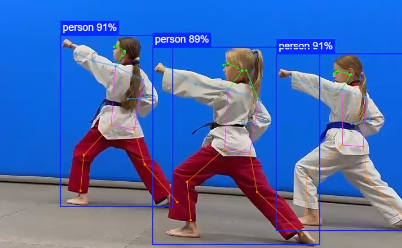
\includegraphics[width=0.75\linewidth]{fig0_test_video}
\caption{Загвар сонголтын туршилтад ашигласан бичлэгийн нэг кадр (илэрсэн хүмүүсийн хүрээ ба араг яс)}
\label{fig:fig0_test_video}
\end{figure}

Бичлэгт гол цэгүүдийн жинхэнэ байрлал (ground truth) тэмдэглэгдээгүй тул гол цэгийн чанарыг шууд бус үзүүлэлтээр үнэлэв. Үүнд: бусад дөрвөн загварын медиантай хэр нийцэж буйг харуулах тохирол (PCK@0.05, биеийн өндрийн 5\%-ийн дотор), дараалсан кадрууд хооронд гол цэг хэр чичирч буйг харуулах чичиргээ (jitter), гар, хөлийн урт бичлэгийн туршид хэр тогтвортой байгааг харуулах мөчдийн уртын хэлбэлзлийн коэффициент.

\textbf{Олон хүний илрүүлэлт.} YOLOv8n, YOLO11n, RTMPose-m, ViTPose-B загварууд кадрын 100\%-д гурван хүнийг бүгдийг нь илрүүлсэн бол MediaPipe зөвхөн 30\%-д нь илрүүлсэн (Зураг~\ref{fig:fig1_detection}). Кадр бүрт илэрсэн хүний тооны графикаас MediaPipe-ийн илрүүлэлт бичлэгийн туршид тасралтгүй хэлбэлзэж байгаа нь харагдана. Бусад загварт хааяа гурваас олон хүн илэрсэн богино хугацааны худал илрүүлэлт ажиглагдсан бөгөөд худал илрүүлэлтгүй кадрын хувь YOLOv8n-д 98.6\%, YOLO11n-д 97.8\%, RTMPose-m болон ViTPose-B-д 97.1\% байв.

\begin{figure}[H]
\centering
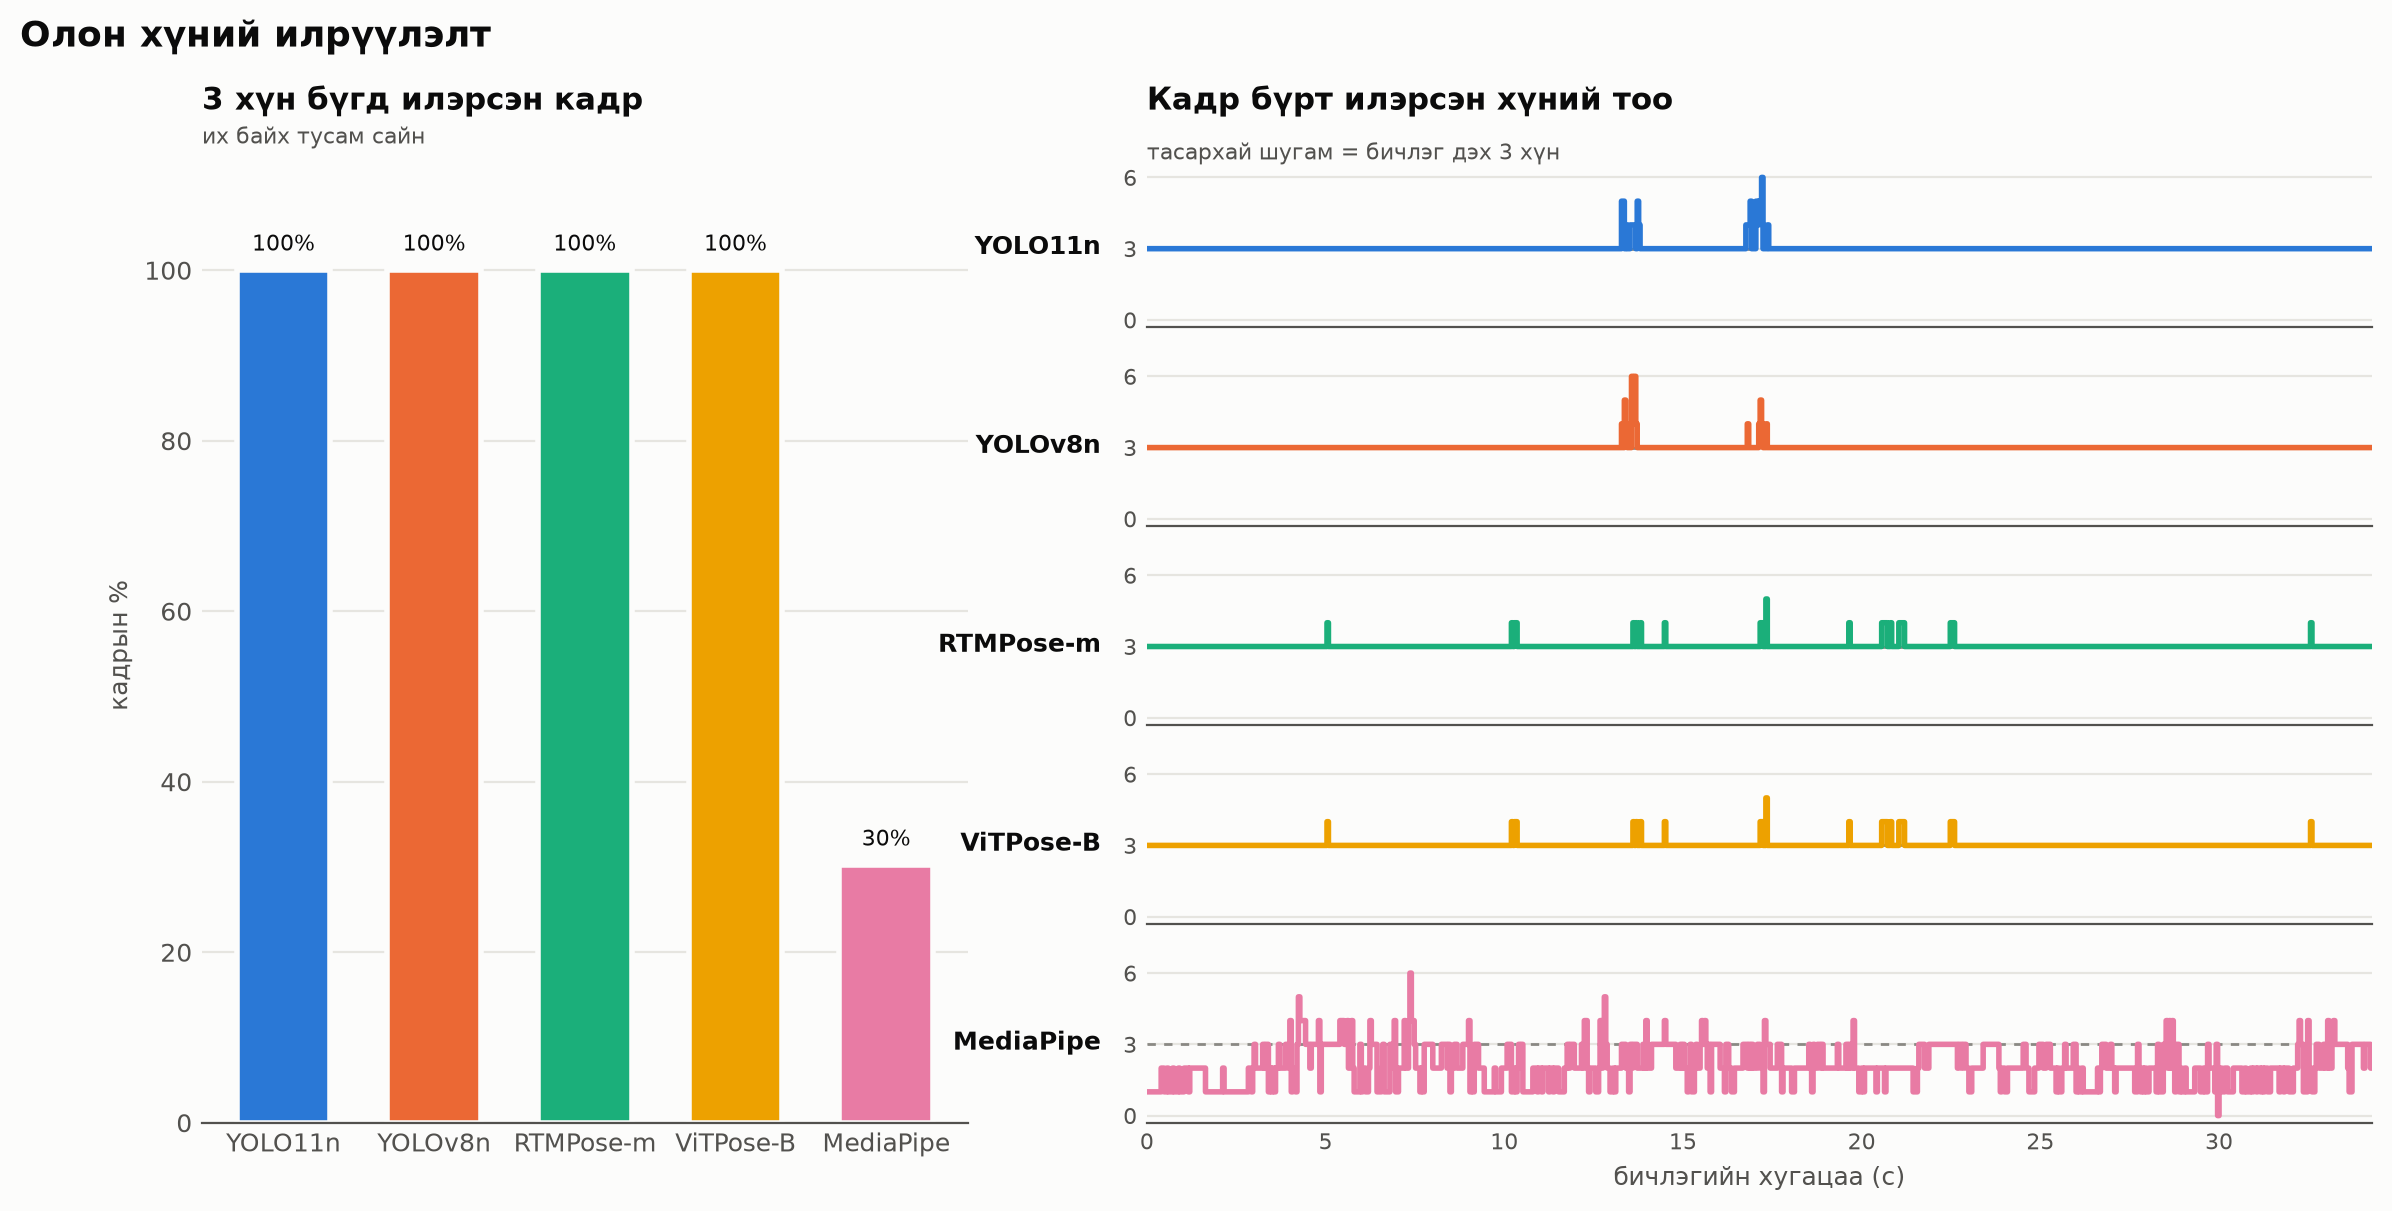
\includegraphics[width=\linewidth]{fig1_detection}
\caption{Гурван хүн бүгд илэрсэн кадрын хувь ба кадр бүрт илэрсэн хүний тоо}
\label{fig:fig1_detection}
\end{figure}

\textbf{Боловсруулалтын хурд.} Нэг кадрын дундаж хугацаа MediaPipe-д 37 мс, YOLOv8n-д 42 мс, YOLO11n-д 46 мс байсан бол RTMPose-m-д 119 мс, ViTPose-B-д 137 мс байв (Зураг~\ref{fig:fig2_speed}). Илэрсэн нэг хүнд ногдох хугацаа RTMPose-m-д 39 мс, ViTPose-B-д 45 мс байгаа нь дээрээс доош загварууд хүн бүрийг тусад нь боловсруулдаг тул хүний тоо нэмэгдэхэд удааширдгийг харуулж байна.

\begin{figure}[H]
\centering
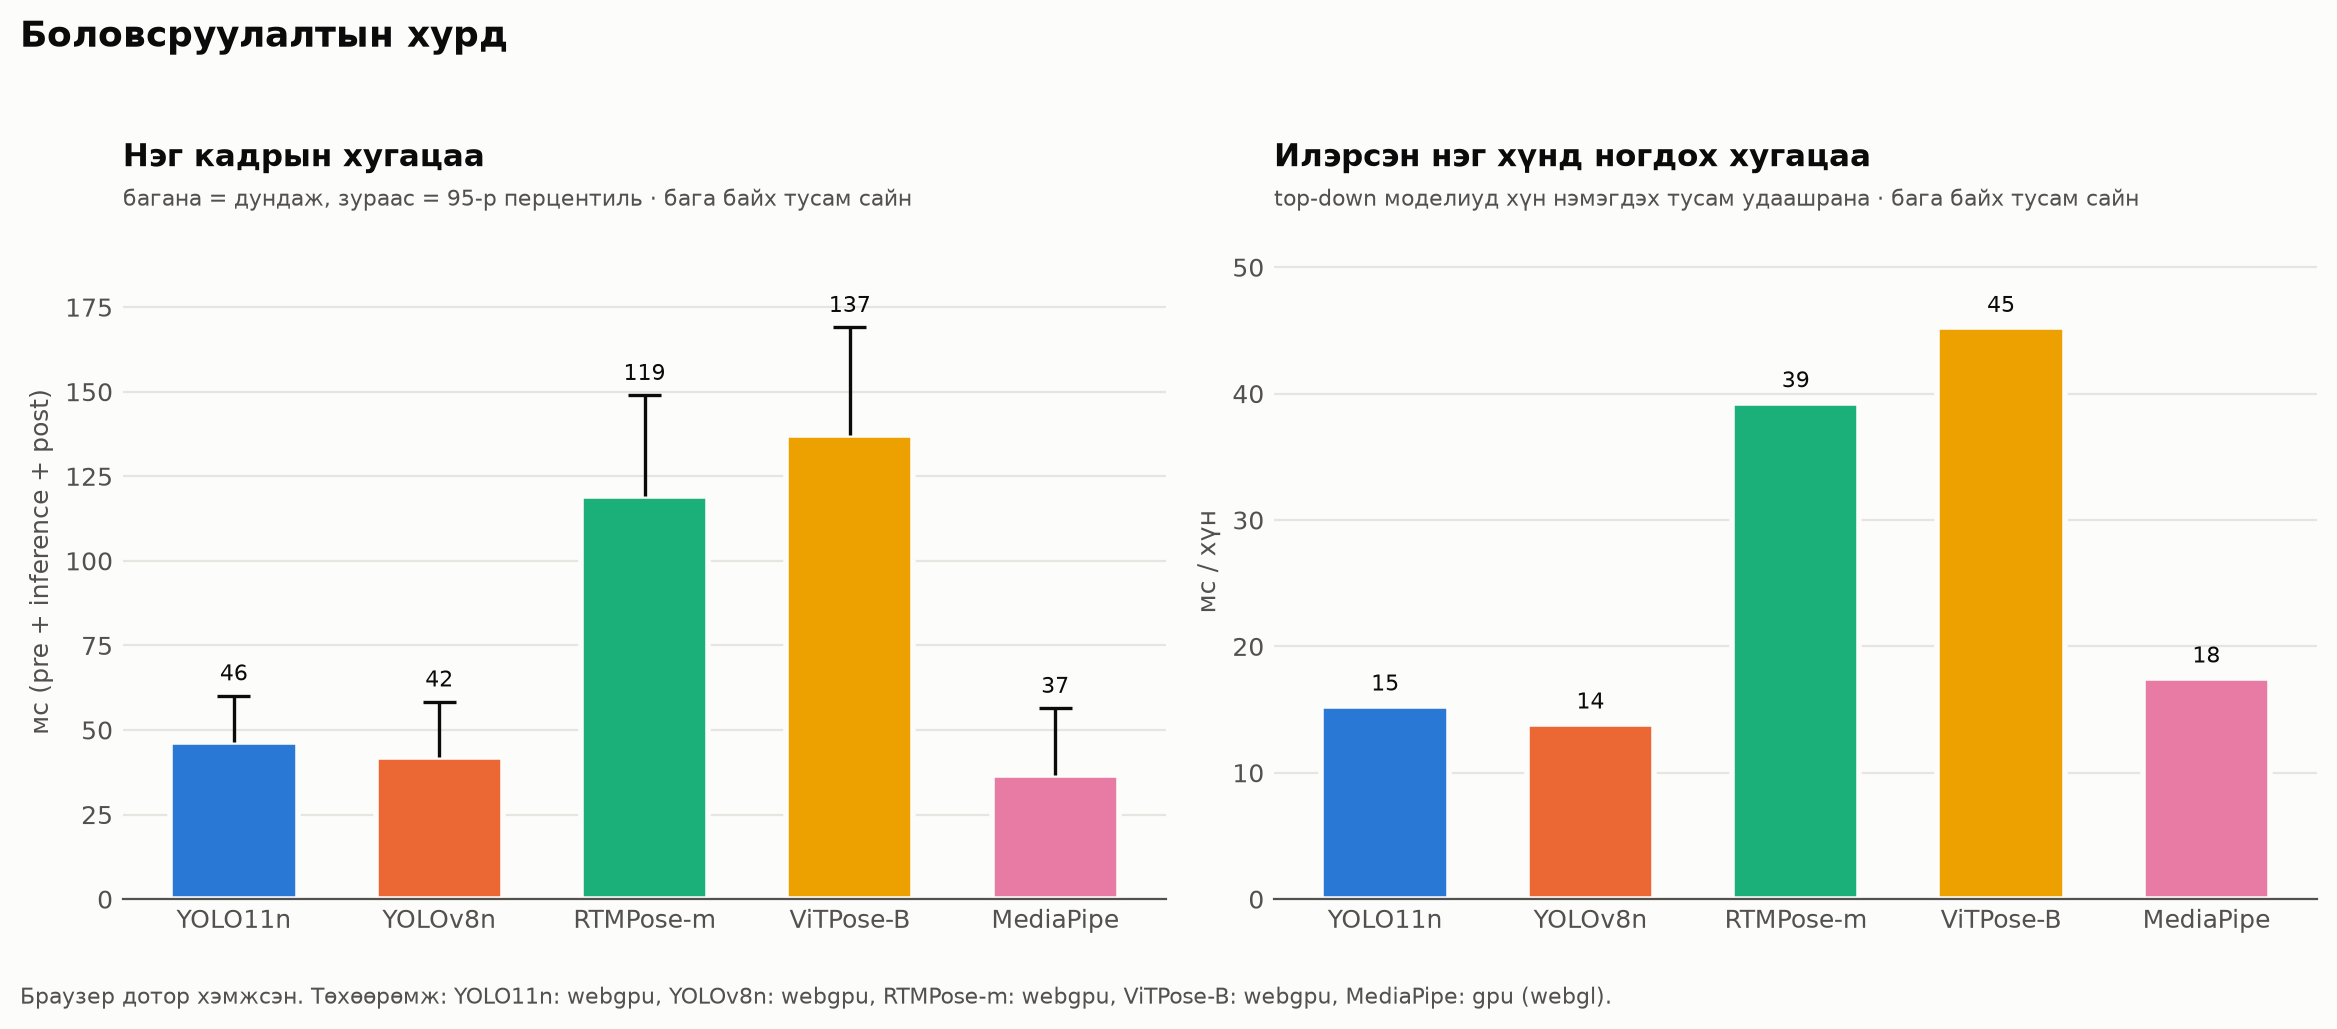
\includegraphics[width=\linewidth]{fig2_speed}
\caption{Нэг кадрын хугацаа (дундаж, 95-р перцентиль) ба илэрсэн нэг хүнд ногдох хугацаа}
\label{fig:fig2_speed}
\end{figure}

\textbf{Гол цэгийн чанар.} Тохирлын хувьд RTMPose-m (93.4\%), ViTPose-B (92.9\%), YOLOv8n (92.5\%), YOLO11n (91.3\%) хоорондоо ойролцоо байсан бол MediaPipe 71.1\%-тай байв (Зураг~\ref{fig:fig3_keypoint_quality}). Чичиргээ хамгийн бага нь RTMPose-m (1.49), хамгийн их нь MediaPipe (9.02) бөгөөд MediaPipe бусад загвараас 4-6 дахин их чичиргээтэй байв. Мөчдийн уртын тогтвортой байдлаар мөн RTMPose-m хамгийн сайн үр дүн (18.7\%) үзүүлсэн.

\begin{figure}[H]
\centering
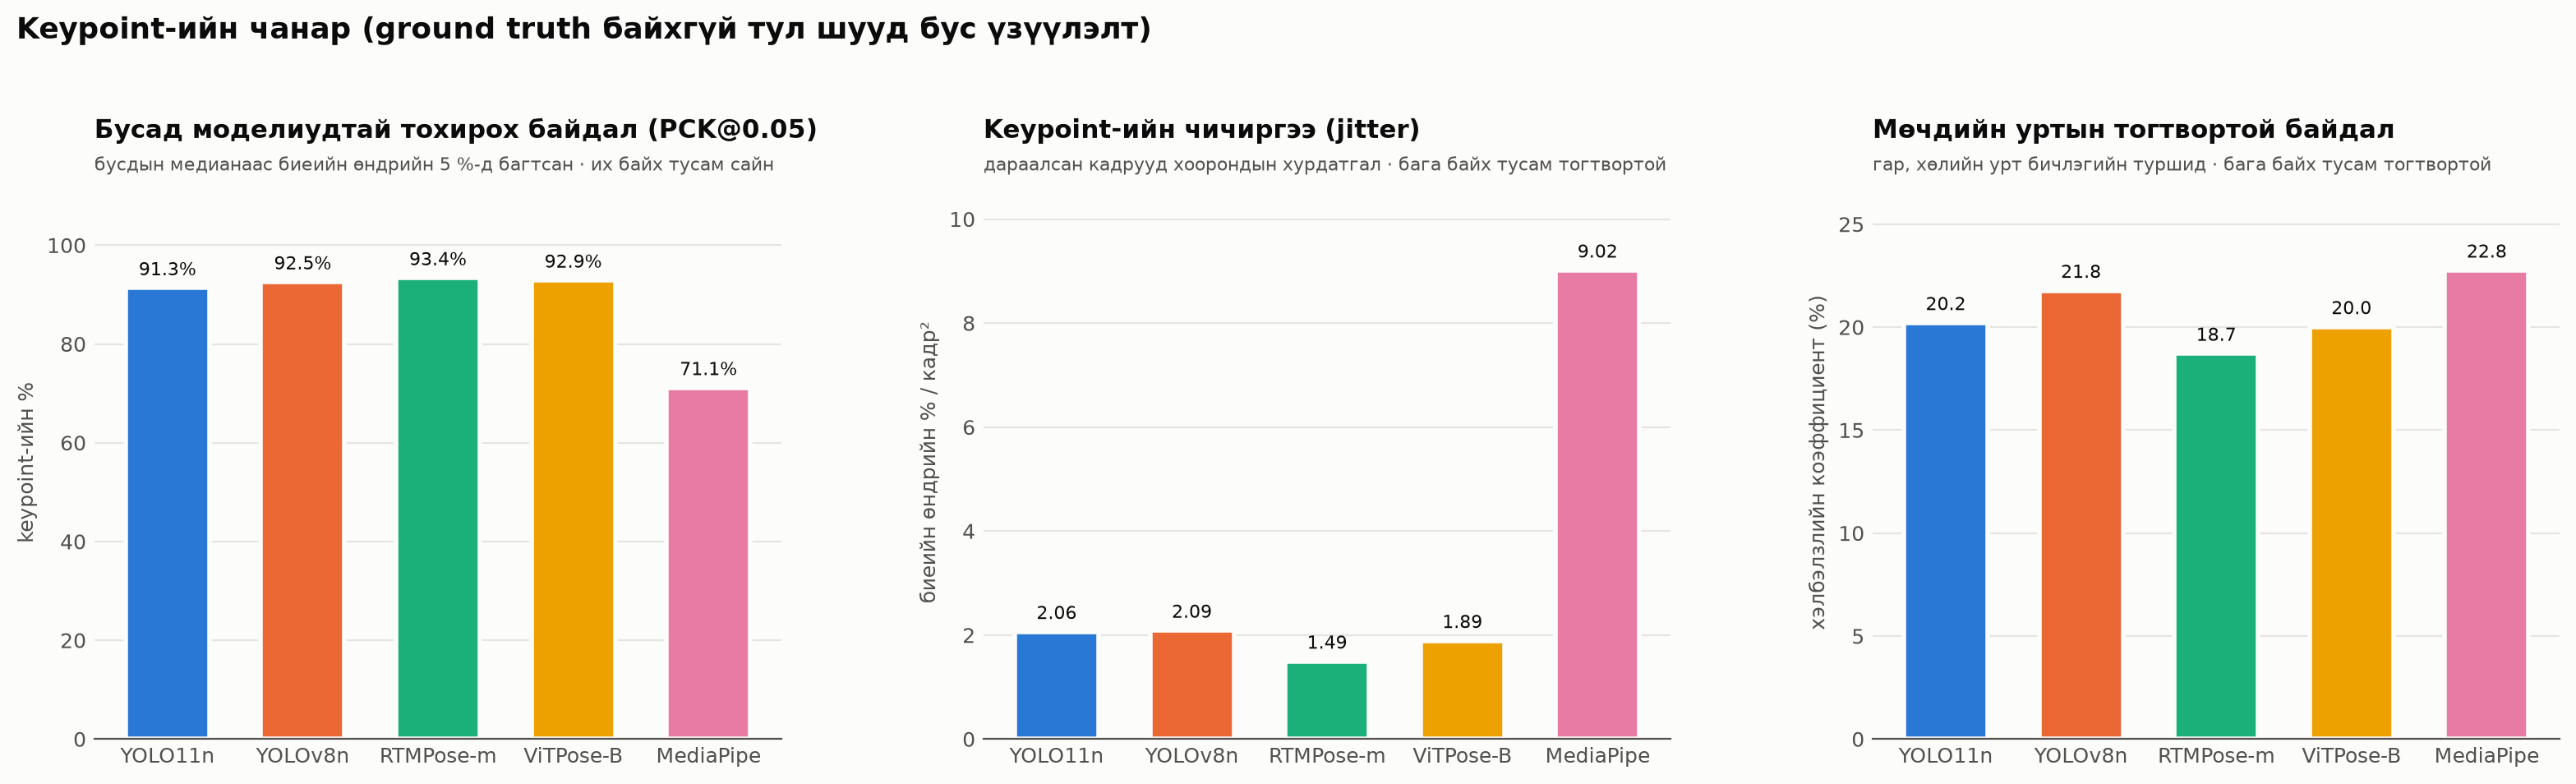
\includegraphics[width=\linewidth]{fig3_keypoint_quality}
\caption{Бусад загваруудтай тохирох байдал, чичиргээ ба мөчдийн уртын тогтвортой байдал}
\label{fig:fig3_keypoint_quality}
\end{figure}

Гол цэг тус бүрээр авч үзвэл бүх загварт бугуй, шагай, тохой, өвдөгний цэгүүд хамгийн их чичиргээтэй, нүүрний цэгүүд хамгийн тогтвортой байв (Зураг~\ref{fig:fig4_keypoint_heatmap}). Энэ нь хөдөлгөөн ихтэй, хурдан хөдөлдөг мөчдийн төгсгөлийн цэгүүдийг илрүүлэх хамгийн хэцүү байдгийг харуулна. Эдгээр цэгүүд нь 3.5-д тодорхойлсон тохой, өвдөгний өнцгийг тооцоолоход шууд ашиглагддаг тул синхрончлолын үнэлгээнд онцгой чухал. Бугуйн чичиргээ RTMPose-m-д 2.6-3.1 байхад YOLO11n-д 4.3-4.5, MediaPipe-д 12.9-13.2 байв.

\begin{figure}[H]
\centering
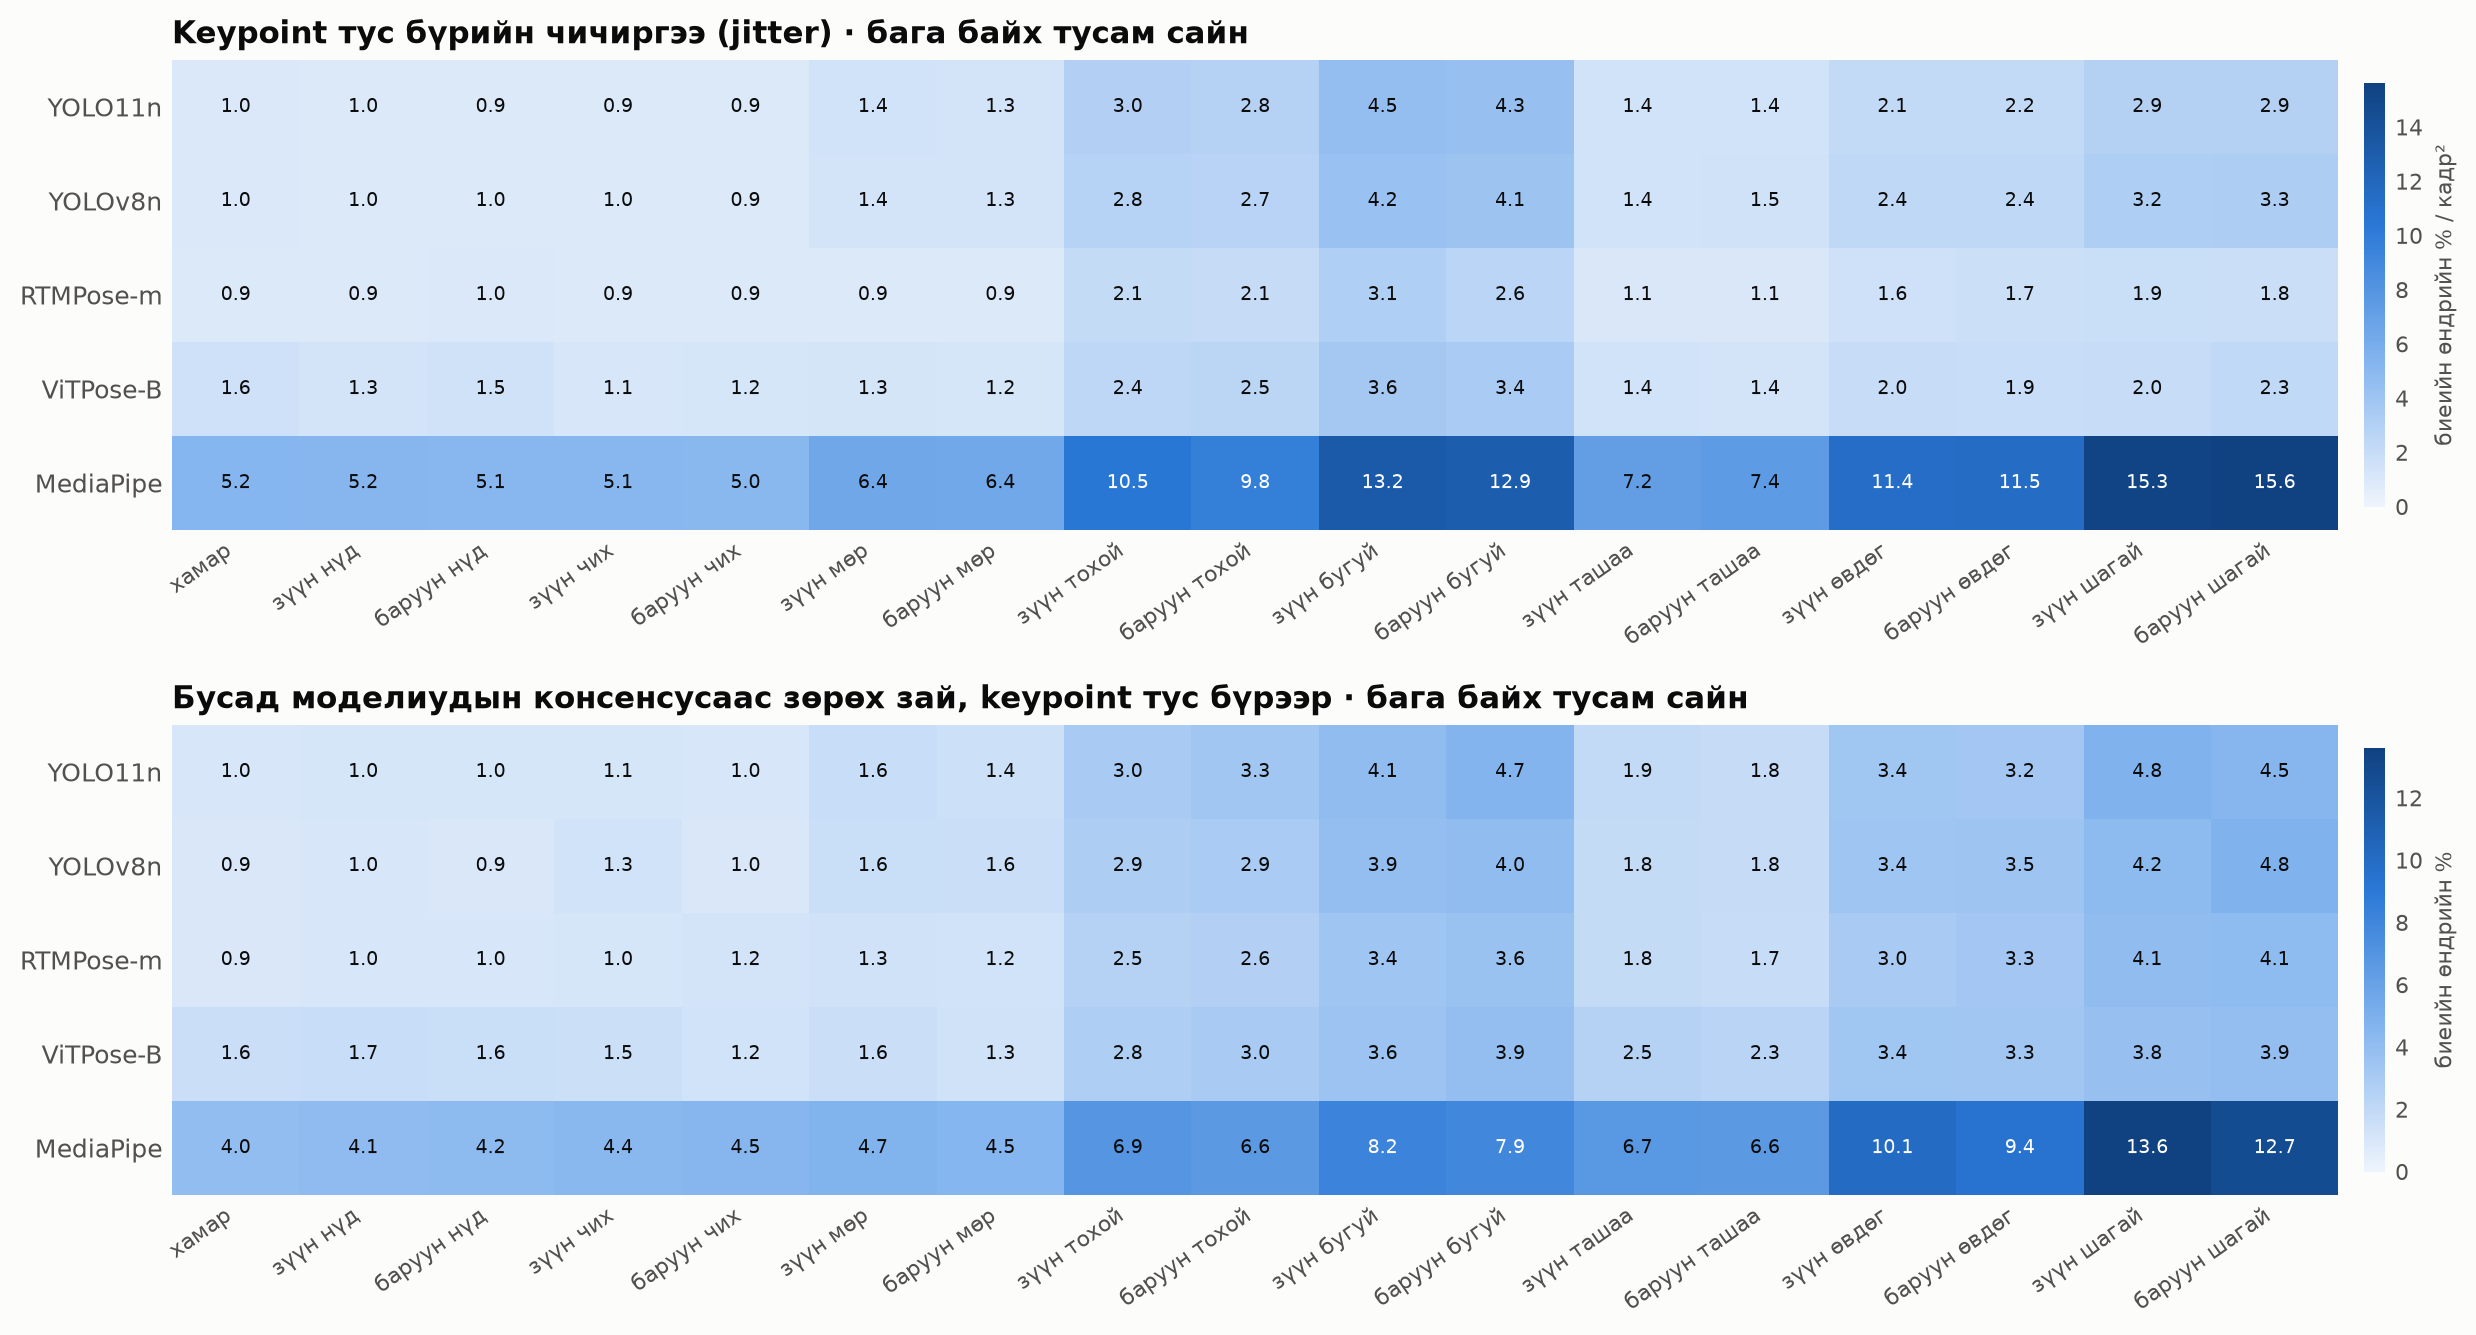
\includegraphics[width=\linewidth]{fig4_keypoint_heatmap}
\caption{Гол цэг тус бүрийн чичиргээ болон бусад загваруудын консенсусаас зөрөх зай}
\label{fig:fig4_keypoint_heatmap}
\end{figure}

\textbf{Хурд ба чанарын харьцаа.} Зураг~\ref{fig:fig5_tradeoff}-д загваруудыг хурд ба тохирлоор нь байршуулсан. YOLOv8n, YOLO11n загварууд хурдан бөгөөд тохирол өндөр, RTMPose-m, ViTPose-B загварууд тохирол бага зэрэг илүү боловч ойролцоогоор гурав дахин удаан, харин MediaPipe хурдан боловч тохирол мэдэгдэхүйц бага байна.

\begin{figure}[H]
\centering
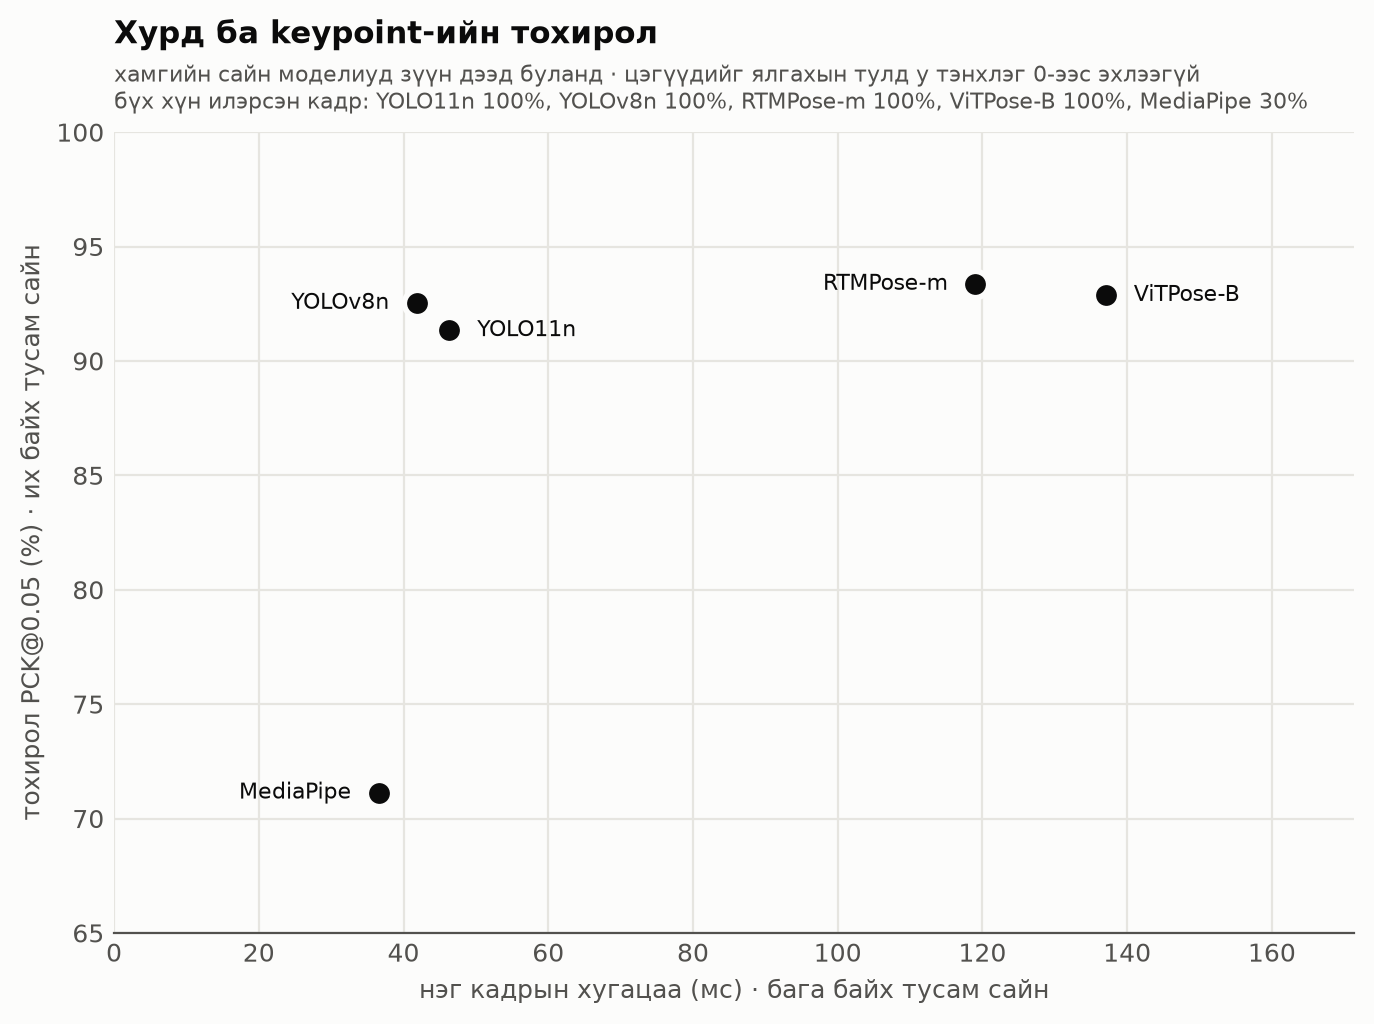
\includegraphics[width=\linewidth]{fig5_tradeoff}
\caption{Хурд ба гол цэгийн тохирлын харьцаа}
\label{fig:fig5_tradeoff}
\end{figure}

\textbf{Нэгдсэн үнэлгээ.} Шалгуур бүрийг хамгийн сайн загварын утгатай харьцуулан (утга ÷ шилдэг утга, бага нь сайн шалгуурт шилдэг утга ÷ утга) 0-1 хооронд хувиргаж, дараах жингээр нэгтгэв: илрүүлэлт 25\%, тохирол 20\%, чичиргээ 20\%, хурд 15\%, худал илрүүлэлт 10\%, мөчдийн тогтвортой байдал 10\%. Анх min-max масштаб ашигласан боловч MediaPipe-ийн хэт муу утгууд бусад дөрвөн загварын хоорондох ялгааг шахаж, MediaPipe-ийг хасахад шилдэг загвар YOLOv8n-ээс RTMPose-m болж өөрчлөгдөж байсан тул харьцааны аргад шилжсэн. Жинлэсэн оноогоор YOLOv8n 91, YOLO11n 90, RTMPose-m 89, ViTPose-B 84, MediaPipe 59 оноо авав (Зураг~\ref{fig:fig6_scorecard}).

\begin{figure}[H]
\centering
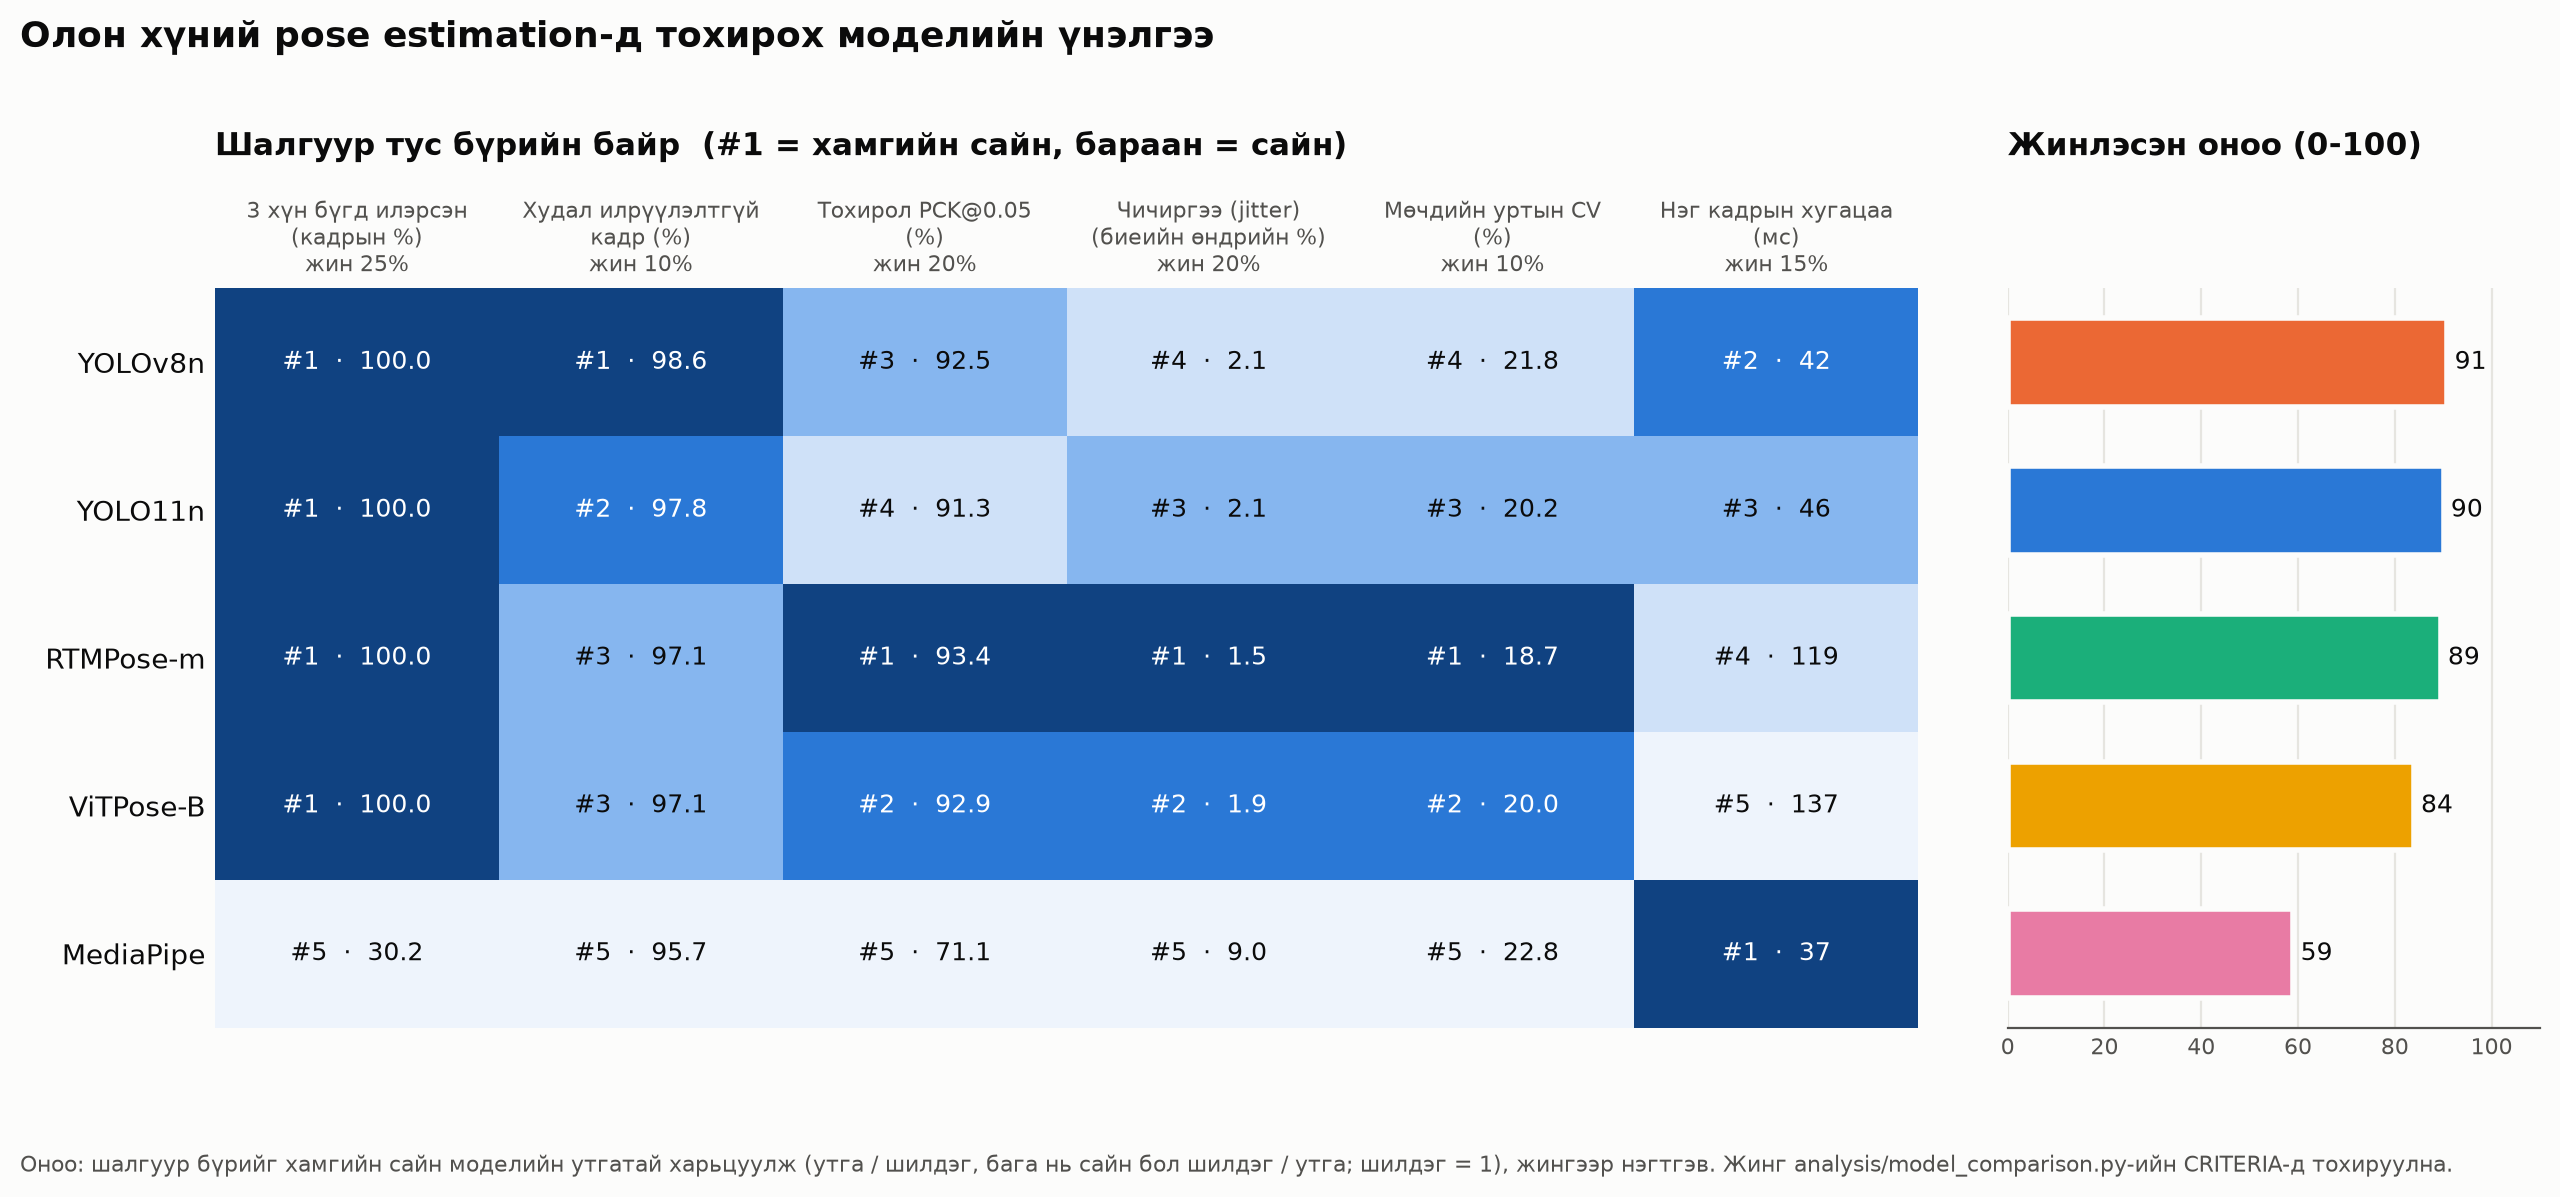
\includegraphics[width=\linewidth]{fig6_scorecard}
\caption{Шалгуур тус бүрийн байр ба жинлэсэн нийт оноо}
\label{fig:fig6_scorecard}
\end{figure}

\textbf{Загвар сонголтын дүгнэлт.} MediaPipe Pose нь нэг хүнд зориулагдсан бөгөөд олон хүнийг тогтвортой илрүүлж чадаагүй тул энэхүү ажилд тохиромжгүй гэж үзэв. Эхний гурван загварын жинлэсэн оноо ердөө 2 онооны зөрүүтэй тул сонголт нь хурд ба гол цэгийн чанарын хоорондын харьцаанаас хамаарна. Энэхүү систем нь шүүгч, дасгалжуулагчдад бичлэгийг дараа нь нарийвчлан шинжлэхэд зориулагдсан бөгөөд тэдний шийдвэр синхрончлолын онооны найдвартай байдлаас шууд хамаарна. Гол цэгийн чичиргээ нь үений өнцгийн хуурамч өөрчлөлт үүсгэж, корреляцид суурилсан оноог бууруулдаг тул хурднаас илүү гол цэгийн чанарыг чухалчлав. Иймд гол цэгийн чанарын бүх үзүүлэлтээр (тохирол 93.4\%, чичиргээ 1.49, мөчдийн уртын хэлбэлзэл 18.7\%), ялангуяа өнцөг тооцоолоход ашиглагдах тохой, бугуй, өвдөг, шагайн цэгүүдийн чичиргээгээр хамгийн сайн үр дүн үзүүлсэн RTMPose-m загварыг сонгов. Жинлэсэн оноогоор YOLOv8n хоёр оноогоор тэргүүлсэн нь хурдны шалгуурт 15\% жин өгсөнтэй холбоотой бөгөөд хурд нь хоёр үе шаттай бүтцийн ачаар (2.6) үр дүнд нөлөөлөхгүй. RTMPose-m-ийн сул тал нь нэг кадрт 119 мс зарцуулж, хүний тоо нэмэгдэхэд удааширдаг явдал боловч хэрэгжүүлэлтийн үндсэн тохиолдол болох хоёр хүнд энэ нь хүлээн зөвшөөрөгдөх хэмжээнд байна.

\textbf{Харьцуулалтын хязгаарлалт.} Ground truth байхгүй тул тохирол нь жинхэнэ нарийвчлал биш, бусад загваруудтай хэр нийцэж буйг л харуулна. Нэг гэр бүлийн загварууд хоорондоо илүү нийцэх хандлагатай бөгөөд YOLOv8n, YOLO11n хоёулаа YOLO гэр бүлийнх, RTMPose-m, ViTPose-B хоёр ижил хүн илрүүлэгч ашигладаг. Шалгууруудын жинг судлаач сонгосон, харьцуулалт нэг бичлэг дээр хийгдсэн, хурдыг браузерийн орчинд хэмжсэн зэргийг үр дүнг тайлбарлахад анхаарах шаардлагатай.

\section{Хүн хуваарилалт}

Бичлэгт хоёр болон түүнээс дээш хүн байх бөгөөд хүмүүс бие биеэ бүрэн халхлахгүй, байраа солихгүй гэж үзнэ. Иймд нарийн мөрдөлтийн (tracking) алгоритм шаардлагагүй бөгөөд кадр бүрт илэрсэн араг ясуудыг гуяны дунд цэгийн x координатаар (гуяны цэгүүд байхгүй үед хүрээний төвөөр) зүүнээс баруун тийш эрэмбэлж, 1, 2, ..., N дугаартай хүнд хуваарилна.

Хүний тоо N-ийг бичлэгийн эхний 2 секундэд хамгийн олон давтагдсан илрүүлэлтийн тоогоор (тэнцүү бол ихийг нь) автоматаар тодорхойлно. Аль нэг кадрт N-ээс олон хүн илэрвэл хүрээний итгэлцэл хамгийн их N илрүүлэлтийг үлдээж, бусдыг нь хасна. N-ээс цөөн хүн илэрвэл илрүүлэлт бүрийг хамгийн сүүлд харагдсан байрлалтай нь хамгийн ойр хүнд шунахай (greedy) аргаар оноож, үлдсэн хүний тухайн кадрын өгөгдлийг дутуу гэж тэмдэглэн 3.4-ийн аргаар нөхнө. Загвар сонголтын бичлэг дээр (856 кадр) 830 кадрт яг гурван хүн, 26 кадрт гурваас олон хүн илэрсэн бөгөөд гурваас цөөн хүн илэрсэн кадр байгаагүй.

\section{Урьдчилсан боловсруулалт}

\textbf{Дутуу ба найдваргүй цэгүүдийг нөхөх.} Итгэлцлийн оноо нь 0.3-аас бага гол цэгүүдийг найдваргүй гэж үзэж, хөрш кадруудын утгаас шугаман интерполяцаар нөхнө. Зөвхөн 1 секундээс богино завсрыг нөхөх бөгөөд үүнээс урт завсар дутуу хэвээр үлдэж, тухайн хугацааны цонхны оноонд оролцохгүй. Загвар сонголтын бичлэг дээр гол цэгийн утгуудын 0.7\%-ийг интерполяцаар нөхсөн.

\textbf{Шуугиан тэгшитгэх.} HPE загварын гаралт кадр бүрт бага зэрэг чичирдэг (jitter) тул координатын цуваа бүрт квадрат олон гишүүнттэй Савицкий-Голейн шүүлтүүр \cite{savitzky1964} хэрэглэнэ. Шүүлтүүрийн цонх ойролцоогоор 0.3 секунд (25 кадр/с давтамжид 9 кадр) бөгөөд хөдөлгөөний хэлбэрийг хадгалахын зэрэгцээ кадр хоорондын санамсаргүй үсрэлтийг бууруулна. Сонгосон RTMPose-m загвар чичиргээ хамгийн багатай байсан ч бугуй, шагайн цэгүүд бусад цэгээс илүү чичирдэг (Зураг~\ref{fig:fig4_keypoint_heatmap}) тул энэ алхам шаардлагатай.

\section{Шинж чанар гаргах}

Кадр бүрт хүн тус бүрийн хувьд дараах найман үений өнцгийг тооцоолно. Өнцөг бүрийг 2.4-т өгсөн томьёогоор гурван гол цэгээс тооцоолно (дугаар нь COCO форматын индекс). Тооцоололд арккосинустай тэнцүү \(\theta = \operatorname{atan2}(|u \times v|, \; u \cdot v)\) хэлбэрийг (\(u = a - b, \; v = c - b\)) ашигласан нь 0° болон 180°-ийн орчимд тоон алдаа багатай.

\begin{table}[H]
\centering
\caption{Үений өнцгийг тооцоолох гол цэгүүд}
\label{tab:joints}
\small
\begin{tabular}{|>{\raggedright\arraybackslash}p{0.234\linewidth}|>{\raggedright\arraybackslash}p{0.260\linewidth}|>{\raggedright\arraybackslash}p{0.372\linewidth}|}
\hline
\textbf{Үе} & \textbf{Гол цэгүүд (a, b, c)} & \textbf{Биеийн хэсэг} \\ \hline
Зүүн тохой & мөр 5, тохой 7, бугуй 9 & Гар \\ \hline
Баруун тохой & мөр 6, тохой 8, бугуй 10 & Гар \\ \hline
Зүүн мөр & гуя 11, мөр 5, тохой 7 & Гар \\ \hline
Баруун мөр & гуя 12, мөр 6, тохой 8 & Гар \\ \hline
Зүүн гуя & мөр 5, гуя 11, өвдөг 13 & Их бие \\ \hline
Баруун гуя & мөр 6, гуя 12, өвдөг 14 & Их бие \\ \hline
Зүүн өвдөг & гуя 11, өвдөг 13, шагай 15 & Хөл \\ \hline
Баруун өвдөг & гуя 12, өвдөг 14, шагай 16 & Хөл \\ \hline
\end{tabular}
\end{table}

Гуяны өнцөг нь мөр, гуя, өвдөг гэсэн цэгүүдээр тодорхойлогддог тул хөл болон их биеийн аль алинд хамаарах боловч биеийн хэсгүүдийн жин давхар тоологдохгүйн тулд их биед хамааруулсан. Ингээд гар нь хоёр тохой ба хоёр мөр (4 үе), хөл нь хоёр өвдөг (2 үе), их бие нь хоёр гуя (2 үе) болно.

\textbf{Биеийн хэсгийн жин.} Синхрончлолын оноонд бүх үеийг тэнцүү тооцохын оронд биеийн хэсгээр (гар, хөл, их бие) хувааж жигнэнэ. Биеийн хэсгийн жинг тухайн хэсгийн үеүдэд тэнцүү хуваарилж, бүх үеийн жингийн нийлбэр 1 болохоор хэвийн болгон үе бүрийн жин \(\alpha_k\)-г гаргана. Энэхүү ажилд гарт 50\%, хөлд 25\%, их биед 25\% жин өгсөн бөгөөд ингэхэд тохой, мөр, өвдөг, гуя тус бүр 12.5\% жинтэй болно. Жингийн утгыг судлаач тогтоосон бөгөөд спортын төрлөөс хамааран өөрчлөх боломжтой.

\section{Синхрончлолын алгоритм}

Синхрончлолыг гурван бүрэлдэхүүн хэсгээр үнэлж, тэдгээрийг нэгтгэн нэг оноо гаргана. Анх төлөвлөсөн аргыг (хувилбар 1) хэрэгжүүлж туршсаны дараа цонхны хэлбэр, үений жин, толин тусгал горимын сонголтыг сайжруулсан бөгөөд энэ хэсэгт эцсийн буюу сайжруулсан хувилбарыг (хувилбар 2) тайлбарлав. Алгоритмын бүх параметрийг секундээр тодорхойлж, видеоны кадрын давтамж f-ээр кадр руу хөрвүүлдэг тул өөр давтамжтай бичлэг дээр ижил утгатай ажиллана.

\textbf{Гулсах цонх.} Кадр бүрт тухайн кадрыг голдоо агуулсан W = 2 секунд урттай нэг цонх (\(t - W/2 \ldots t + W/2\)) үүсгэнэ. Бичлэгийн эхлэл, төгсгөлд цонх видеоноос гарах тул түүнийг видеоны дотор шилжүүлж, урт нь W хэвээр үлдэнэ. Ингэснээр бүрэлдэхүүн бүрийн оноо кадр бүрт тодорхойлогдож, видеог тоглуулахад тухайн мөчийн оноог цагийн тэмдгээр шууд харуулах боломжтой болно.

\textbf{Байрлалын ижил төстэй байдал.} Цонхонд хоёр хүний харгалзах үений өнцгийн абсолют зөрүүний дунджийг үе бүрээр тооцоолж, үений жингээр нэгтгэнэ:

\begin{equation}
S_{pose} = 1 - \sum_{k=1}^{K} \alpha_k \frac{\bar{d}_k}{180^{\circ}}, \qquad \bar{d}_k = \frac{1}{|T_k|} \sum_{t \in T_k} \left| \theta^{A}_{k}(t) - \theta^{B}_{k}(t) \right|
\end{equation}

Энд \(T_k\) нь цонхны k үеийн хоёр хүнд хоёуланд нь утгатай кадрууд бөгөөд өгөгдөлгүй үеийг хасаж, үлдсэн үеүдийн жинг нийлбэр нь 1 болохоор дахин хэвийн болгоно. Цонхны утгуудын тал хувиас бага нь байгаа бол тухайн цонхонд оноо өгөхгүй.

\textbf{Хөдөлгөөний уялдаа.} Цонхонд үе тус бүрийн өнцгийн цуваануудын Пирсоны корреляц \(r_k\)-г тооцоолж, үений жингээр нэгтгэнэ:

\begin{equation}
S_{corr} = \frac{1}{2} \left( \sum_{k} \alpha_k r_k + 1 \right)
\end{equation}

Хоёр хүнд хоёуланд нь өнцгийн стандарт хазайлт 3°-аас бага, өөрөөр хэлбэл бараг хөдөлгөөнгүй үеийн корреляц нь шуугианаас хамаардаг тул түүнийг \(S_{corr}\) болон хоцрогдлын тооцооллоос хасна. Нэг хүн тухайн үеэ хөдөлгөж, нөгөө нь хөдөлгөөгүй бол \(r_k = 0\) гэж үзнэ. Цонхонд аль ч үе хөдлөөгүй, өөрөөр хэлбэл хоёр хүн хоёулаа байрлалаа барьж зогссон бол корреляц болон хоцрогдол тодорхойгүй тул оноог зөвхөн \(S_{pose}\)-оор гаргана.

\textbf{Цагийн хоцрогдол.} Хоёр хүний өнцгийн өөрчлөлтийн хурдны (кадр хоорондын ялгавар) цуваанд хэвийн болгосон хөндлөн корреляцыг хэрэглэж, хөдөлж буй үеүдийн \(\rho(\tau)\)-ийн дундаж хамгийн их байх \(\tau^{*}\) шилжилтийг \(|\tau| \le \tau_{max}\) мужид олно. Тэнцүү утгатай бол хамгийн бага \(|\tau|\)-г сонгоно. Хоцрогдлын оноог дараах байдлаар тооцоолно:

\begin{equation}
S_{lag} = \begin{cases} \max\left(0, \; 1 - \dfrac{|\tau^{*}|}{\tau_{max}}\right), & \rho_{max} \ge \rho_{min} \\ 0, & \rho_{max} < \rho_{min} \end{cases}
\end{equation}

Хоёр хүн огт өөр хөдөлгөөн хийсэн үед хөндлөн корреляц санамсаргүй нэг шилжилтийг «хамгийн сайн» гэж сонгодог тул \(\rho_{min}\) босгоор олдсон хоцрогдолд итгэх эсэхийг шийднэ. Хамгийн их хайх хоцрогдол \(\tau_{max} = 1.5\) секунд бөгөөд энэ нь туршсан хамгийн их хоцрогдлоос (1 секунд) их байх ёстой. Босгын утгыг загвар сонголтын бичлэг дээр гол цэгийн түвшний хяналттай хосоор тохируулсан. Хамт хөдөлж буй хүмүүсийн цонхнуудын \(\rho_{max}\)-ийн медиан ойролцоогоор 0.42, өөр хөдөлгөөнтэй хосынх 0.13, яг ижил хуулбарынх 1.0 байв. Иймд төлөвлөж байсан 0.5 босго бодит синхрон хөдөлгөөнийг ч үгүйсгэж байсан тул хоёр бүлгийг ялгах \(\rho_{min} = 0.3\) утгыг сонгов. Энэ босгын орчимд \(S_{lag}\) огцом өөрчлөгддөг сул талтай болох нь хожим илэрсэн бөгөөд үүнийг 4.4-т тайлбарлав.

\textbf{Нэгдсэн оноо.} Гурван бүрэлдэхүүнийг жигнэсэн нийлбэрээр нэгтгэж, 0-100 хуваарьт шилжүүлнэ:

\begin{equation}
S = 100 \cdot \left( w_1 S_{pose} + w_2 S_{corr} + w_3 S_{lag} \right), \qquad w_1 + w_2 + w_3 = 1
\end{equation}

Бүрэлдэхүүнүүд \(w_1 = w_2 = w_3 = 1/3\) тэнцүү жинтэй бөгөөд аль нэг бүрэлдэхүүн тодорхойгүй үед (жишээлбэл, хөдөлгөөнгүй цонх) үлдсэн бүрэлдэхүүнүүдийн жинг дахин хэвийн болгоно. Хосын бүх бичлэгийн оноо нь цонхнуудын онооны дундаж, бүх бичлэгийн хоцрогдол нь бүтэн цувааны хөндлөн корреляцаар олдсон \(\tau^{*}\) байна. Биеийн хэсэг бүрийн (гар, хөл, их бие) оноог зөвхөн тухайн хэсгийн үеүдийг тэнцүү жинтэйгээр ашиглан ижил аргаар тооцоолж, аль хэсэгт синхрончлол алдагдаж байгааг тодорхойлно.

\textbf{Хоёр горимт харьцуулалт.} Бүжгийн найруулга ердийн эсвэл толин тусгал байхаас хамааран харьцуулах арга өөр болно (2.4). Иймд цонх бүрт ердийн болон толин тусгал (Б хүний зүүн, баруун үеүдийг сольсон) гэсэн хоёр горимоор оноо тооцоолно. Толин тусгал горимын оноо ердийн горимынхоос дор хаяж 5 оноогоор их байвал л толин тусгал горимыг сонгож, бусад тохиолдолд ердийн горимыг хэрэглэнэ. Энэ нь хоёр горимын оноо ойролцоо байх үед горим цонх бүрээр солигдож анивчихаас сэргийлэхээс гадна нэг бүжигчин санамсаргүй буруу гараа хөдөлгөхөд систем үүнийг толин тусгал гэж үзэж алдааг нуух эрсдэлийг бууруулна. Найруулгын горим урьдчилан мэдэгдэж байгаа тохиолдолд хэрэглэгч горимыг тогтмол сонгох боломжтой.

\textbf{Олон хүний синхрончлол.} Дээрх тооцоолол нь хоёр хүний хоорондох синхрончлолыг үнэлдэг бөгөөд энэ нь аргын үндсэн бөгөөд хамгийн оновчтой тохиолдол юм. Бичлэгт N хүн байх үед бүлэгт гол хүн (дасгалжуулагч, ахлагч) байхгүй, бүх хүн тэгш эрхтэй гэж үзэж, хүн бүрийг бусад бүх хүнтэй хос хосоор нь харьцуулна. Хосын тоо \(N(N-1)/2\) бөгөөд гурван хүнд 3, дөрвөн хүнд 6 хос болно. i ба j хүний хоорондох синхрончлолын оноог \(S_{ij}\) гэвэл бүлгийн нийт оноог бүх хосын онооны дунджаар, i-р хүний оноог түүний оролцсон хосуудын онооны дунджаар тооцоолно:

\begin{equation}
S_{group} = \frac{2}{N(N-1)} \sum_{i<j} S_{ij}, \qquad S_i = \frac{1}{N-1} \sum_{j \ne i} S_{ij}
\end{equation}

Хүн тус бүрийн оноо \(S_i\) нь бүлгээсээ хамгийн их зөрж буй хүнийг тодорхойлох боломж олгоно. Хоёр горимт харьцуулалт болон хоцрогдлын тооцоолол хос бүрт тусдаа хийгдэнэ. Хосын тоо хүний тоотой квадратаар өсдөг боловч тооцоолол нь өнцгийн цуваан дээр хийгдэх тул HPE загварын тооцооллоос хамаагүй бага бөгөөд гурван хүнтэй 856 кадрын бичлэгийн синхрончлолыг бүхэлд нь хэдхэн секундэд тооцоолж байна.

\textbf{Синхрончлол алдагдсан мөчүүд.} Бүлгийн нэг тоон оноо нь хэзээ, хэн, биеийн аль хэсгээрээ зөрснийг харуулдаггүй тул хос бүрт синхрончлол алдагдсан хугацааны хэсгүүдийг (мөчүүдийг) тусад нь илрүүлнэ. Цонхыг дараах нөхцлийн аль нэг биелэхэд «зөрсөн» гэж тэмдэглэнэ. Үүнд:

\begin{itemize}
\item
  Цонхны \(S_{corr}\) нь тухайн хосын бүх бичлэгийн медианаас 0.15-аар, эсвэл \(S_{pose}\) нь медианаас 0.06-аар бага байх. Хос бүрийг өөрийнх нь ердийн түвшинтэй харьцуулдаг тул байнга бага зэрэг зөрдөг хос нэг урт мөч болж харагдахгүй.
\item
  Бүх бие найдвартай хоцорсон байх: \(|\tau^{*}| \ge 0.2\) секунд ба \(\rho_{max} \ge \rho_{min}\).
\item
  Аль нэг мөч (зүүн, баруун гар нь тохой ба мөр, зүүн, баруун хөл нь гуя ба өвдөг) хоцорсон байх. Хоёр дахь хүний тухайн мөчийг τ-гаар шилжүүлэхэд өнцгийн дундаж зөрүү \(D(\tau)\) мэдэгдэхүйц багасвал, өөрөөр хэлбэл \(D(0) - \min D(\tau) \ge 3^{\circ}\) ба \(D(0)\)-ийн 20\%-иас их, мөн \(0.2 \le |\tau| < \tau_{max}\) секунд байвал мөчийг хоцорсон гэж үзнэ. Энэ нөхцөл нь нэг гар хоцорч, бусад хэсэг нь зэрэг хөдөлж буй, бүх биеийн оноонд дундажлагдан алга болдог тохиолдлыг илрүүлнэ.
\end{itemize}

Нийт 1 секундээс урт хугацааг хамарсан зөрсөн цонхнууд (0.5 секундээс богино завсрыг нэгтгэж) нэг мөч болно. Мөч бүрт хоцорсон мөч болон хоцрогдлыг, мөн хоцорсон мөчийн үе бүрийн хувьд тухайн шилжилт зөрүүг 2°-аас их багасгасан эсэхийг (хоцорсон үе), эсвэл өнцгийн зөрүү нь бичлэгийн ердийн зөрүүнээс 15°-аас их байгаа эсэхийг (өөр хөдөлгөөнтэй үе) тодорхойлж харуулна. «Хоцорсон» гэж тооцох доод хоцрогдол нь анхдагчаар 0.2 секунд бөгөөд хэрэглэгч үүнийг 0.12--1.0 секундийн хооронд өөрчилж болох ч энэ нь зөвхөн жагсаах мөчүүдэд нөлөөлж, оноог өөрчлөхгүй. 0.12 секундээс бага утгад синхрон хосын цонхнуудад ч хэмжигддэг 0.04--0.16 секундийн хоцрогдол мөч болж тоологдон, бичлэгийн бараг тал нь зөрсөн гэж тэмдэглэгдэж байсан тул доод хязгаарыг 0.12 секунд болгосон.

Алгоритмын эхний (хувилбар 1) болон сайжруулсан (хувилбар 2) хувилбарын ялгааг доорх хүснэгтэд нэгтгэв.

\begin{table}[H]
\centering
\caption{Синхрончлолын алгоритмын хувилбаруудын ялгаа}
\label{tab:versions}
\small
\begin{tabular}{|>{\raggedright\arraybackslash}p{0.200\linewidth}|>{\raggedright\arraybackslash}p{0.320\linewidth}|>{\raggedright\arraybackslash}p{0.360\linewidth}|}
\hline
\textbf{Шинж} & \textbf{Хувилбар 1} & \textbf{Хувилбар 2} \\ \hline
Цонх & 3 секунд, 0.5 секунд тутамд & 2 секунд, кадр бүрт, кадр голдоо \\ \hline
Үений жин & Бүх үе тэнцүү & Биеийн хэсгийн жингээс \(\alpha_k\) (гар 50\%, хөл 25\%, их бие 25\%) \\ \hline
Биеийн хэсэг & Хөл = гуя ба өвдөг, их бие = гуя & Хөл = өвдөг, их бие = гуя (давхардалгүй) \\ \hline
Толин тусгал & Өндөр оноотой горимыг сонгоно & 5 оноогоор илүү бол л толин тусгал \\ \hline
Гаралт & Цонх бүрийн CSV & Нэмээд кадр бүрийн CSV (цагийн тэмдэгтэй) \\ \hline
\end{tabular}
\end{table}

Хувилбар 2-ын ерөнхий бүтцийг доорх хуурмаг кодоор (pseudocode) харуулав.

\begin{lstlisting}[language=Python, caption={Синхрончлолын алгоритмын хуурмаг код (хувилбар 2)}, label={lst:sync}, frame=single, columns=fullflexible, keepspaces=true]
def group_sync(frames, fps, W=2.0, tau_max=1.5, rho_min=0.3,
               w=(1/3, 1/3, 1/3), part_weights=GENERAL, margin=5):
    N = most_common_count(frames, first_seconds=2)
    people = assign_left_to_right(frames, N)           # гуяны x-ээр 1..N
    people = [preprocess(p) for p in people]           # нөхөх, тэгшитгэх
    angles = [joint_angles(p) for p in people]         # хүн бүрт (8, T)
    alpha = joint_weights(part_weights)                # alpha_k, нийлбэр 1

    S = zeros((N, N))
    for i, j in combinations(range(N), 2):             # хос бүр
        frame_scores = []
        for t in range(len(frames)):                   # кадр бүрт нэг цонх
            win = centred_window(t, W * fps)
            s_n = window_score(angles[i], angles[j], win, alpha)
            s_m = window_score(angles[i], mirror(angles[j]), win, alpha)
            frame_scores.append(s_m if s_m >= s_n + margin else s_n)
        S[i, j] = S[j, i] = mean(frame_scores)
    group = mean([S[i, j] for i, j in combinations(range(N), 2)])
    per_person = [sum(S[i]) / (N - 1) for i in range(N)]
    return group, per_person

def window_score(a, b, win, alpha):
    s_pose = 1 - weighted_mean(abs(a[:, win] - b[:, win]), alpha) / 180
    moving = [k for k in range(8) if std(a[k, win]) >= 3 or std(b[k, win]) >= 3]
    if not moving:
        return 100 * s_pose                            # хоёулаа хөдөлгөөнгүй
    s_corr = (weighted_mean(pearson(a[k, win], b[k, win]) for k in moving) + 1) / 2
    tau, rho_max = normalized_cross_corr(diff(a), diff(b), win, moving, tau_max)
    s_lag = max(0, 1 - abs(tau) / tau_max) if rho_max >= rho_min else 0
    return 100 * (w[0] * s_pose + w[1] * s_corr + w[2] * s_lag)
\end{lstlisting}

\section{Хэрэгжүүлэлтийн орчин}

Системийг 2.6-д тайлбарласан технологиудаар хэрэгжүүлсэн. Хэрэглэгч видеог аль орчинд боловсруулахаа хуудсан дээрх «Process videos on: This browser / Server» сонголтоор шийднэ.

\textbf{Вэб хөтчийн горим.} RTMPose-m загвар болон түүний YOLO11n хүн илрүүлэгчийг ONNX Runtime Web сангаар WebGPU backend дээр (боломжгүй үед WASM) ажиллуулна. Видеог кадр бүрээр уншиж, загварын гаралтаас араг яс зурагдсан видео, үр дүнгийн файлуудыг үүсгэнэ.

\textbf{Серверийн горим.} Вэб аппликейшн нээлттэй байгаа видео файлыг Python серверт илгээж, сервер ижил ONNX файлуудыг ONNX Runtime-ээр CUDA (NVIDIA GPU) дээр, боломжгүй үед CPU дээр ажиллуулна. Серверийн боловсруулалт нь хөтчийнхтэй ижил алхмуудаас бүрдэнэ. Үүнд: хүн илрүүлэгчийн оролтыг 640×640 хэмжээнд харьцааг нь хадгалан багасгаж саарал (114) өнгөөр дүүргэх, зөвхөн хүний ангиллыг авч давхацсан илрүүлэлтүүдийг IoU 0.7 босготой NMS-ээр шүүх, хүрээг 1.25 дахин томруулж загварын харьцаанд тааруулан 192×256 хэмжээнд тайрах, ImageNet-ийн дундаж, стандарт хазайлтаар хэвийн болгох, SimCC гаралтаас x, y тэнхлэг тус бүрийн хамгийн их утгаар гол цэгийг тодорхойлох. Видеог OpenCV-ээр кадр бүрээр, алгасахгүйгээр уншиж, хөтчийн хадгалдагтай яг ижил бүтэцтэй гол цэгийн JSON буцаана. Сервер зөвхөн гол цэгийг тодорхойлох бөгөөд синхрончлол, статистик, үр дүн хадгалах ажлыг вэб аппликейшн хөтчийн горимтой адил гүйцэтгэдэг тул хоёр горимын үр дүн шууд харьцуулагдана. Араг яс зурагдсан видеог буцаасан гол цэгүүдээс хөтөч дээр зурна. Серверийн API-ийг доорх хүснэгтэд үзүүлэв.

\begin{table}[H]
\centering
\caption{HPE серверийн API}
\label{tab:api}
\small
\begin{tabular}{|>{\raggedright\arraybackslash}p{0.330\linewidth}|>{\raggedright\arraybackslash}p{0.560\linewidth}|}
\hline
\textbf{Хүсэлт} & \textbf{Үүрэг} \\ \hline
\texttt{GET /health} & Серверийн төлөв, загварууд болон тэдгээрийн ажиллах төхөөрөмж \\ \hline
\texttt{POST /jobs} & Видео, загварын нэр, итгэлцлийн босго, кадрын давтамж, кадрын тоог хүлээн авч ажлын дугаар буцаана \\ \hline
\texttt{GET /jobs/\{id\}} & Ажлын төлөв (дараалалд, ажиллаж байна, дууссан, алдаа) ба явцын хувь \\ \hline
\texttt{GET /jobs/\{id\}/keypoints} & Кадр бүрийн гол цэгүүд (хөтчийн форматаар) \\ \hline
\texttt{DELETE /jobs/\{id\}} & Ажлыг цуцалж устгах \\ \hline
\end{tabular}
\end{table}

GPU нэгэн зэрэг олон ажлыг гүйцэтгэхэд удаашрах тул сервер ажлуудыг дараалалд оруулж нэг нэгээр нь гүйцэтгэх бөгөөд илгээсэн видеог ажил дуусмагц устгана. Үр дүнгийн JSON файлд тухайн ажиллуулалт аль горимд хийгдсэн (\texttt{backend}), серверийн горимд видео илгээх болон серверийн боловсруулалтын хугацааг хадгалдаг тул хоёр горимын хурд, үр дүнг дараа нь харьцуулах боломжтой.

\textbf{Үр дүнгийн файлууд.} Ажиллуулалт бүр гол цэгийн JSON, CSV, кадр бүрийн хүний тоо, загварын харьцуулалтын хэмжүүрүүд, араг яс зурагдсан MP4 видео болон синхрончлолын үр дүнг үүсгэнэ. Синхрончлолын үр дүнд бүх бичлэгийн дүн (JSON), хос бүрийн цонхны оноо (CSV), кадр бүрийн оноо (CSV; цагийн тэмдэг, бүлгийн оноо, хүн тус бүрийн оноо, хос бүрийн оноо, хоцрогдол мс-ээр, горим, гар, хөл, их биеийн оноо) болон кадр бүрийн үений өнцөг (CSV) багтана. Ижил бичлэгийг дахин боловсруулахад өмнөх файлуудыг дарж бичихгүй, шинэ дугаартай файл үүсгэнэ.

\textbf{Туршилтын хэрэгслүүд.} Синхрончлолын алгоритм нь вэб хөтөч болон Node.js орчинд хоёуланд ажиллахаар бичигдсэн тул хадгалсан гол цэгийн файлууд дээр алгоритмыг тушаалын мөрөөс параметрүүдийг нь өөрчлөн дахин ажиллуулах боломжтой. Туршилтын үр дүнгийн шинжилгээ болон тайлангийн графикуудыг Python хэл дээр Pandas, NumPy, Matplotlib сангуудаар гаргана.

\chapter{Өгөгдөл ба туршилт}
\section{Туршилтын өгөгдөл}

Шаардлагад нийцсэн, синхрончлолын түвшин нь тэмдэглэгдсэн бодит олон хүний бичлэг олох боломж хязгаарлагдмал тул алгоритмыг голчлон хяналттай (синтетик) өгөгдөл дээр үнэлж, дараа нь бодит бичлэгүүд дээр шалгав. Хяналттай өгөгдлийн давуу тал нь хүмүүсийн хоорондох ялгааг (хоцрогдол, зай, байрлал гэх мэт) судлаач өөрөө тогтоодог тул алгоритмын үр дүнг жинхэнэ утгатай шууд харьцуулах боломжтой явдал юм.

\textbf{Хяналттай өгөгдөл үүсгэх арга.} Нэг хүний хөдөлгөөнийг агуулсан бичлэгийг эх сурвалж болгон авч, түүний хуулбарыг хоёр дахь хүн болгон эх бичлэгийн хажууд нь нэг кадрт зэрэгцүүлэн нийлүүлсэн. Иймд 1-р хүн (зүүн тал) нь эх бичлэг, 2-р хүн (баруун тал) нь өөрчилсөн хуулбар бөгөөд жинхэнэ хариу урьдчилан мэдэгдэнэ. Эх бичлэг нь нэг балетчны 13.9 секунд үргэлжлэх, 960×1080 нягтаршилтай, 30 кадр/с давтамжтай бичлэг бөгөөд тогтмол давтамжтай болгох үүднээс 25 кадр/с (347 кадр) руу хөрвүүлсэн. Балетын хөдөлгөөнд гар, хөл хоёулаа идэвхтэй оролцдог тул үений бүх өнцгийг шалгахад тохиромжтой. Хуулбарт хийсэн өөрчлөлтүүдийг FFmpeg программын шүүлтүүрүүдээр үүсгэсэн (Хүснэгт~\ref{tab:synthetic}).

\begin{table}[H]
\centering
\caption{Хяналттай өгөгдөл үүсгэсэн өөрчлөлтүүд}
\label{tab:synthetic}
\small
\begin{tabular}{|>{\raggedright\arraybackslash}p{0.150\linewidth}|>{\raggedright\arraybackslash}p{0.260\linewidth}|>{\raggedright\arraybackslash}p{0.230\linewidth}|>{\raggedright\arraybackslash}p{0.230\linewidth}|}
\hline
\textbf{Өөрчлөлт} & \textbf{Хэрхэн үүсгэсэн (FFmpeg)} & \textbf{Утгууд} & \textbf{Шалгасан зүйл} \\ \hline
Цагийн хоцрогдол & Хуулбарын эхэнд эхний кадрыг давтаж хойшлуулах (\texttt{tpad}) & 0, 1, 2, 3, 5, 8, 12, 25 кадр (0--1 секунд) & Хоцрогдол тодорхойлох нарийвчлал, онооны өөрчлөлт \\ \hline
Толин тусгал & Хуулбарыг хэвтээ чиглэлд эргүүлэх (\texttt{hflip}) & 0 ба 8 кадрын хоцрогдолтой & Хоёр горимт харьцуулалт \\ \hline
Өөр хөдөлгөөн & Хуулбарыг эх бичлэгийн өөр хэсгээс эхлүүлэх & 4, 7, 10 секундийн зөрүүтэй & Хоцрогдлын итгэлцлийн шалгалт \\ \hline
Камерын зай & Хуулбарыг жижигрүүлж доод талд нь байрлуулах (\texttt{scale}, \texttt{pad}) & 100, 75, 50, 25\%, 0 ба 8 кадрын хоцрогдолтой & Өнцөгт суурилсан арга зайнаас үл хамаарах эсэх \\ \hline
Нягтаршил & Хосын бичлэгийг багасгах (\texttt{scale}) & 1080p, 720p, 480p, 360p, 240p, 8 кадрын хоцрогдолтой & Гол цэг болон онооны тогтвортой байдал \\ \hline
Кадрын давтамж & 30 кадр/с хосын бичлэгийг бууруулах (\texttt{fps}) & 30, 25, 15, 10 кадр/с, 0.3 секундийн хоцрогдолтой & Хоцрогдлын нарийвчлал \\ \hline
Хүний тоо & Эх бичлэгийн 2, 3, 4 хуулбарыг зэрэгцүүлэх, сүүлийнхийг хоцроох & 2, 3, 4 хүн, 8 кадрын хоцрогдолтой & Бүлгээсээ зөрж буй хүнийг илрүүлэх, хурд \\ \hline
\end{tabular}
\end{table}

Байрлалын шилжилтийг тусад нь шалгаагүй. Учир нь үений өнцөг нь кадр дахь байрлалаас математикийн хувьд хамааралгүй бөгөөд хосын бичлэг бүрт хоёр хүн аль хэдийн кадрын өөр хэсэгт байрладаг.

\textbf{Гол цэгийн түвшний хяналттай өгөгдөл.} Видеог дахин боловсруулахгүйгээр алгоритмыг HPE-ийн алдаанаас тусгаарлан шалгахын тулд бодит бичлэгийн гол цэгийн цуваанд шууд өөрчлөлт оруулав. Тухайлбал, нэг хүний бүх бие эсвэл нэг, хоёр мөчийн гол цэгийг тодорхой хугацаанд хоцроох, мөн тухайн хүний хөдөлгөөнийг бичлэгийн өөр хэсгийнхээр солих.

\textbf{Бодит бичлэг.} Бодит нөхцөлд шалгахдаа загвар сонголтын бичлэг (гурван хүн тулааны урлагийн ижил хөдөлгөөн хийсэн, 720×1280, 25 кадр/с, 856 кадр) болон гурван бүжигчин хамтдаа бүжиглэсэн дөрвөн бичлэгийг (1920×1080, 59.94 кадр/с, 31--43 секунд) ашигласан. Эдгээр бичлэгийн синхрончлолын жинхэнэ түвшин тэмдэглэгдээгүй тул үр дүнг чанарын хувьд тайлбарлав.

\textbf{Боловсруулалт.} Хяналттай болон бодит бүх бичлэгийг RTMPose-m загвараар (хүн илрүүлэгчийн итгэлцлийн босго 0.25) HPE серверт (CUDA, NVIDIA GeForce RTX 2060) боловсруулж, синхрончлолыг хувилбар 2-ын анхдагч тохиргоогоор тооцоолсон. Бичлэг үүсгэх, серверт боловсруулах, оноо тооцоолж CSV файлд хадгалах бүх алхмыг нэг скриптээр автоматжуулсан тул туршилтыг бүхэлд нь дахин гүйцэтгэх боломжтой.

\section{Үнэлгээний хэмжүүрүүд}

\begin{table}[H]
\centering
\caption{Үнэлгээний хэмжүүрүүд}
\label{tab:metrics}
\small
\begin{tabular}{|>{\raggedright\arraybackslash}p{0.234\linewidth}|>{\raggedright\arraybackslash}p{0.260\linewidth}|>{\raggedright\arraybackslash}p{0.372\linewidth}|}
\hline
\textbf{Хэмжүүр} & \textbf{Юуг үнэлэх} & \textbf{Сайн үр дүн} \\ \hline
Нөхцөл хоорондын ялгаа & Синхрон, хоцрогдолтой, өөр хөдөлгөөнтэй бичлэгүүдийн оноо зөв дараалалд ялгарч буйг & Синхрон \textgreater{} хоцрогдолтой \textgreater{} өөр хөдөлгөөн \\ \hline
Онооны тогтвортой байдал & Ижил нөхцөлтэй бичлэгүүдийн оноо хэр ойролцоо гарч буйг & Бага зөрүү \\ \hline
Хоцрогдлын алдаа (мс) & Тооцоолсон хоцрогдол жинхэнэ хоцрогдлоос хэр зөрж буйг & 0-д ойр \\ \hline
Гол цэгийн тохирол (PCK@0.05) & Нягтаршил буурахад гол цэг жишиг бичлэгийнхээс хэр зөрж буйг & 100\%-д ойр \\ \hline
Боловсруулалтын хурд & Нэг кадрын хугацаа (мс), бодит хурд (кадр/с) & Бага хугацаа \\ \hline
\end{tabular}
\end{table}

\headshort{Хөтөч ба сервер}
\section{Вэб хөтөч ба серверийн боловсруулалт}

Загвар сонголтын бичлэгийг (856 кадр, 25 кадр/с) RTMPose-m загвараар вэб хөтөч дээр (WebGPU) болон сервер дээр (CUDA) боловсруулж харьцуулав (Хүснэгт~\ref{tab:browser_server}, Зураг~\ref{fig:fig7_browser_vs_server}).

\begin{table}[H]
\centering
\caption{Вэб хөтөч ба серверийн боловсруулалтын харьцуулалт}
\label{tab:browser_server}
\small
\begin{tabular}{|>{\raggedright\arraybackslash}p{0.420\linewidth}|>{\raggedright\arraybackslash}p{0.220\linewidth}|>{\raggedright\arraybackslash}p{0.220\linewidth}|}
\hline
\textbf{Үзүүлэлт} & \textbf{Вэб хөтөч} & \textbf{Сервер} \\ \hline
Тооцооллын төхөөрөмж & WebGPU & CUDA \\ \hline
Нэг кадрын хугацаа, дундаж (мс) & 113.8 & 50.8 \\ \hline
Нэг кадрын хугацаа, 95-р перцентиль (мс) & 160.3 & 83.8 \\ \hline
Бодит хурд (кадр/с) & 5.5 & 17.4 \\ \hline
Гурван хүн бүгд илэрсэн кадр & 100\% & 100\% \\ \hline
Гурваас олон хүн илэрсэн кадр & 3.0\% & 4.0\% \\ \hline
Гол цэгийн дундаж итгэлцэл & 0.709 & 0.711 \\ \hline
Чичиргээ (хүрээний өндрийн \%) & 1.46 & 1.48 \\ \hline
Мөчдийн уртын хэлбэлзэл (\%) & 18.7 & 18.9 \\ \hline
Бүлгийн синхрончлолын оноо & 82.6 & 81.4 \\ \hline
\end{tabular}
\end{table}

Серверийн бодит хурдад видео илгээх (0.1 секунд) болон боловсруулалтын хугацааг оруулсан бөгөөд хөтөч дээр араг яс зурах, видео кодчилох хугацаа мөн орсон. Сервер вэб хөтчөөс 2.2 дахин хурдан ажилласан. Хоёр горимд ижил хүмүүсийн гол цэгүүдийн хоорондох зай медианаар 0.61 пиксел, 95-р перцентилээр 2.25 пиксел, дунджаар хүний хүрээний өндрийн 0.29\% байв. Кадруудын 98.6\%-д илэрсэн хүний тоо ижил байсан бөгөөд аль ч горимд гурваас цөөн хүн илэрсэн кадр байгаагүй тул ялгаа нь гурваас олон хүн илэрсэн (26 ба 34) кадруудад гарсан. Ийм бага зөрүү нь хоёр орчинд видео задлах (OpenCV ба вэб хөтөч) болон зургийн хэмжээ өөрчлөх аргын ялгаанаас гарна. Харин бүлгийн синхрончлолын оноо 1.2 оноогоор зөрсөн бөгөөд шалтгааныг 4.4-т тайлбарлав.

\begin{figure}[H]
\centering
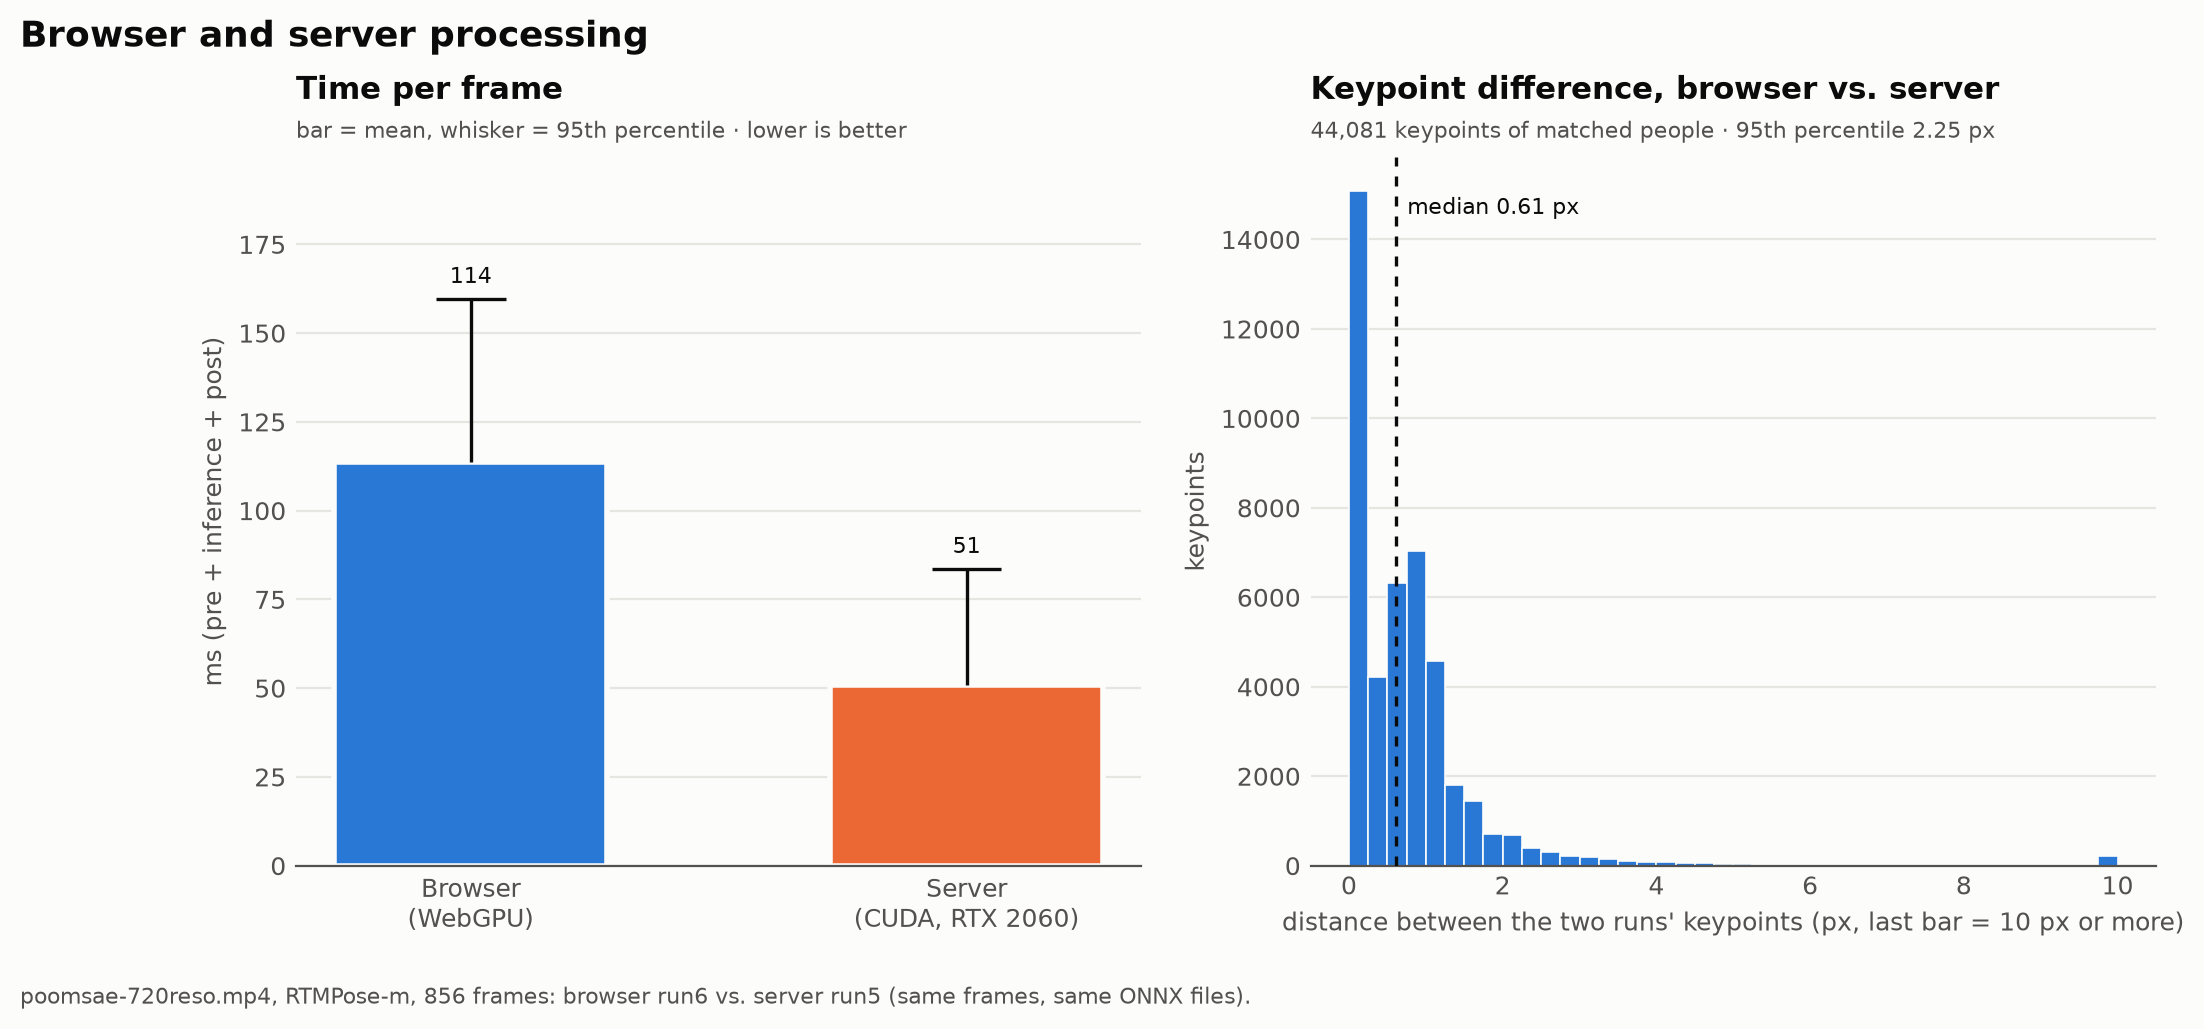
\includegraphics[width=\linewidth]{fig7_browser_vs_server}
\caption{Вэб хөтөч ба серверийн нэг кадрын хугацаа болон гол цэгийн зөрүүний тархалт}
\label{fig:fig7_browser_vs_server}
\end{figure}

\textbf{Кадр унших алдаа ба түүний засвар.} Хоёр горимыг харьцуулах явцад вэб хөтчийн кадр унших аргад алдаа илэрсэн. Анхны хэрэгжүүлэлтэд i-р кадрыг уншихдаа видеог яг \(i/f\) хугацаа руу шилжүүлдэг байв. Кадрын яг хил дээр шилжихэд Chrome хөтөч заримдаа өмнөх кадрыг харуулдаг тул 30 кадр/с давтамжтай бичлэгт уншсан кадрын дугаарууд 0, 1, 1, 3, 4, 4, 6, \ldots{} буюу гурван кадр тутмын нэг нь давхардаж, нэг нь алгасагдаж байв. Мөн эхний кадрын цагийн тэмдэг нь 0.04 секунд байсан загвар сонголтын бичлэгт бүх кадр нэг кадраар хоцорч, 856 кадрын оронд 858 кадр боловсруулагдсан. Засварын дараа видеог кадрын голд, өөрөөр хэлбэл эхний кадрын цагийн тэмдэг \(+ (i + 0.5)/f\) хугацаа руу шилжүүлдэг болсноор i-р ажиллуулалтын кадр нь видеоны жинхэнэ i-р кадртай тохирч, сервер ч мөн ижил кадруудыг уншдаг болсон. Энэ засвараас өмнө хийсэн 3.2-ын загваруудын харьцуулалт болон загвар бүрийн нягтаршлын туршилтад энэ алдаа нөлөөлсөн. Бүх загвар ижил аргаар хэмжигдсэн тул загваруудын харьцангуй дүгнэлт хүчинтэй боловч чичиргээний үнэмлэхүй утга бага зэрэг өөр байж болзошгүй. Энэ бүлгийн бусад бүх туршилтыг засварын дараа серверээр хийсэн тул алдаанд өртөөгүй.

\headshort{Алгоритмын туршилт}
\section{Синхрончлолын алгоритмын туршилт}

\textbf{Цагийн хоцрогдол.} Хуулбарыг 0--25 кадраар (0--1 секунд) хоцроосон найман бичлэг дээр алгоритм бүх бичлэгийн хоцрогдлыг найман тохиолдол бүгдэд нь яг зөв, өөрөөр хэлбэл 0 мс алдаатай олсон (Хүснэгт~\ref{tab:lag_test}, Зураг~\ref{fig:fig11_lag}). Хамгийн их корреляц \(\rho_{max}\) бүх тохиолдолд 0.95-аас их тул олдсон хоцрогдол бүгд найдвартай гэж тэмдэглэгдсэн.

\begin{table}[H]
\centering
\caption{Видеоны түвшний хоцрогдлын туршилтын үр дүн (1--2 хос)}
\label{tab:lag_test}
\small
\begin{tabular}{|>{\raggedright\arraybackslash}p{0.110\linewidth}|>{\raggedright\arraybackslash}p{0.105\linewidth}|>{\raggedright\arraybackslash}p{0.085\linewidth}|>{\raggedright\arraybackslash}p{0.085\linewidth}|>{\raggedright\arraybackslash}p{0.085\linewidth}|>{\raggedright\arraybackslash}p{0.085\linewidth}|>{\raggedright\arraybackslash}p{0.110\linewidth}|>{\raggedright\arraybackslash}p{0.085\linewidth}|}
\hline
\textbf{Хоцрогдол (кадр)} & \textbf{Жинхэнэ (с)} & \(S\) & \(S_{pose}\) & \(S_{corr}\) & \(S_{lag}\) & \textbf{Олдсон (с)} & \(\rho_{max}\) \\ \hline
0 & 0 & 99.8 & 0.996 & 0.998 & 1.000 & 0 & 0.98 \\ \hline
1 & 0.04 & 97.1 & 0.968 & 0.972 & 0.974 & 0.04 & 0.96 \\ \hline
2 & 0.08 & 93.1 & 0.939 & 0.906 & 0.947 & 0.08 & 0.97 \\ \hline
3 & 0.12 & 89.0 & 0.916 & 0.832 & 0.921 & 0.12 & 0.97 \\ \hline
5 & 0.20 & 80.9 & 0.879 & 0.681 & 0.868 & 0.20 & 0.97 \\ \hline
8 & 0.32 & 71.8 & 0.839 & 0.525 & 0.789 & 0.32 & 0.99 \\ \hline
12 & 0.48 & 64.4 & 0.812 & 0.436 & 0.684 & 0.48 & 0.96 \\ \hline
25 & 1.00 & 54.3 & 0.798 & 0.485 & 0.344 & 1.00 & 0.95 \\ \hline
\end{tabular}
\end{table}

\begin{figure}[H]
\centering
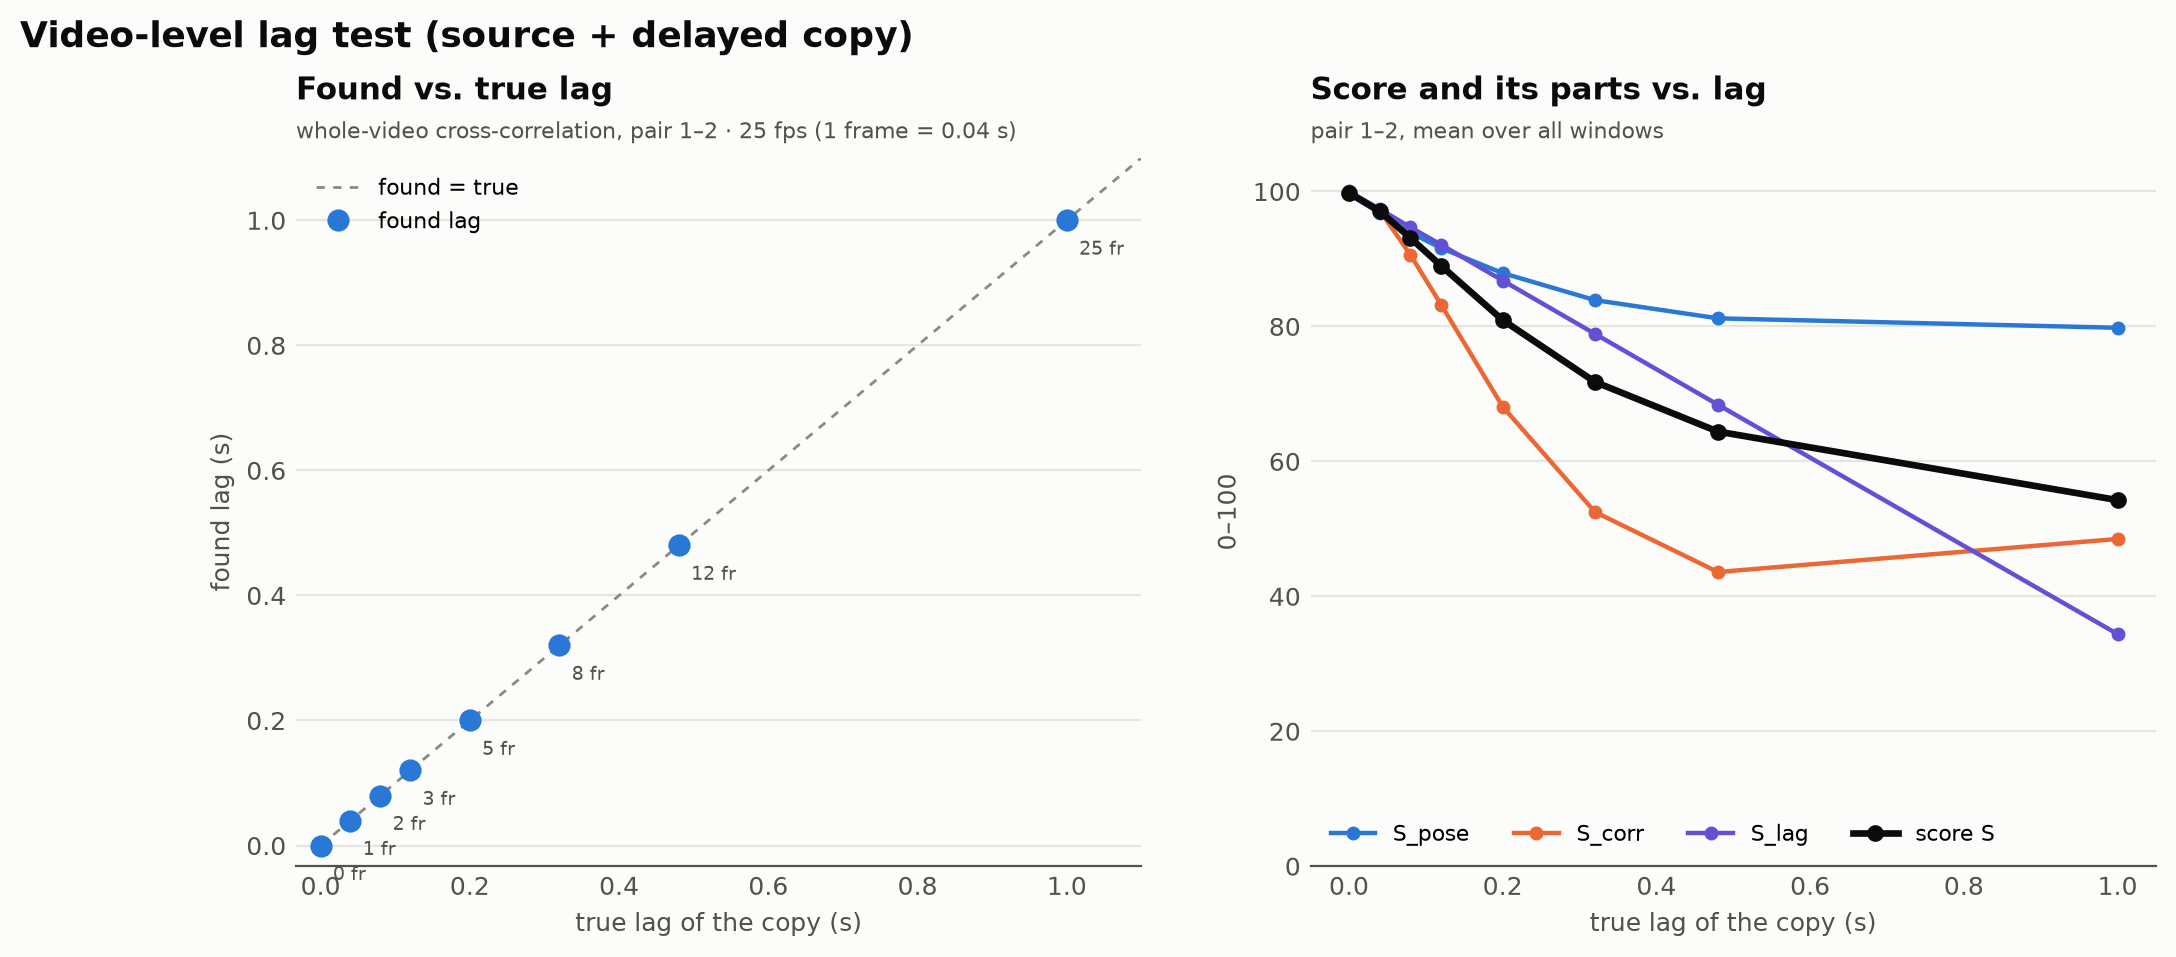
\includegraphics[width=\linewidth]{fig11_lag}
\caption{Олдсон ба жинхэнэ хоцрогдол, мөн хоцрогдлоос хамаарах оноо ба түүний бүрэлдэхүүнүүд}
\label{fig:fig11_lag}
\end{figure}

Хоцрогдол нэмэгдэх тусам нэгдсэн оноо 99.8-аас 54.3 хүртэл жигд буурсан. Бүрэлдэхүүн тус бүрээр авч үзвэл хөдөлгөөний уялдаа \(S_{corr}\) хамгийн мэдрэмтгий бөгөөд 0.2 секундийн хоцрогдолд 0.68 хүртэл буурсан бол байрлалын ижил төстэй байдал \(S_{pose}\) аажуухан буурч, 0.48 секундээс хойш бараг тогтмол болсон. Хоцрогдлын оноо \(S_{lag}\) нь \(1 - |\tau^{*}|/\tau_{max}\) томьёоны дагуу шугаман буурсан. Синхрончлол алдагдсан мөч нь 0.2 секунд ба түүнээс их хоцрогдолтой бичлэгүүдэд бүх бичлэгийг хамарч, зөв хоцрогдолтойгоор илэрсэн бөгөөд 0.12 секундээс бага хоцрогдолд илрээгүй нь «хоцорсон» гэж тооцох анхдагч 0.2 секундийн босготой тохирч байна.

\textbf{Толин тусгал ба өөр хөдөлгөөн.} Хэвтээ чиглэлд эргүүлсэн хуулбарын хувьд цонхнуудын 100\%-д толин тусгал горим сонгогдож, оноо 99.3 буюу синхрон бичлэгтэй бараг тэнцүү гарсан. Толин тусгал хуулбарыг 8 кадраар хоцроосон үед оноо 71.5 болж, хоцрогдол мөн 0.32 секунд гэж зөв олдсон. Харин эх бичлэгийн өөр хэсгийн хөдөлгөөнөөр солиход оноо 4, 7, 10 секундийн зөрүүд харгалзан 62.0, 53.7, 45.4 болж буурсан бөгөөд бүх тохиолдолд \(\rho_{max}\) нь 0.11--0.22 буюу \(\rho_{min} = 0.3\)-аас бага тул бүх бичлэгийн хоцрогдлыг найдваргүй гэж зөв тэмдэглэсэн (Зураг~\ref{fig:fig12_conditions}).

\begin{figure}[H]
\centering
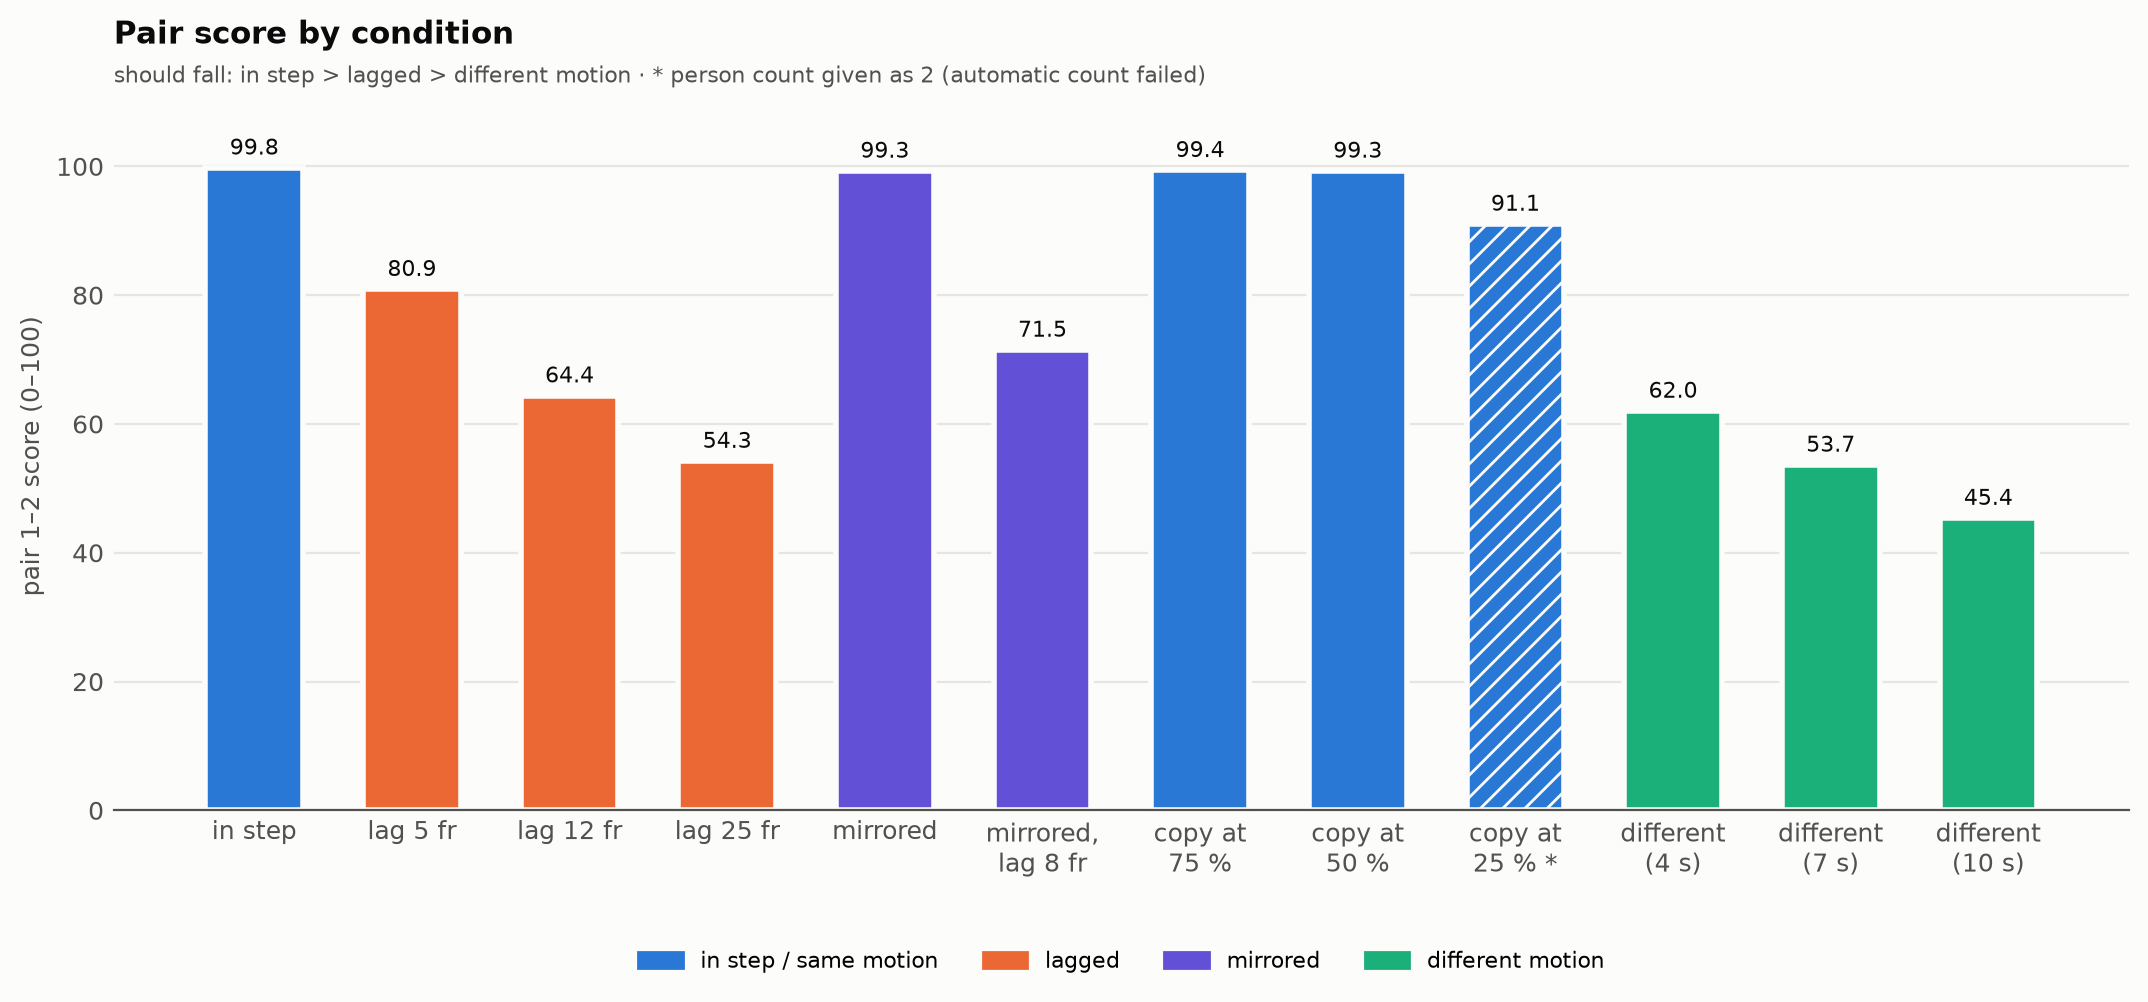
\includegraphics[width=\linewidth]{fig12_conditions}
\caption{Нөхцөл тус бүрийн 1--2 хосын оноо}
\label{fig:fig12_conditions}
\end{figure}

Нөхцлүүдийн оноо синхрон (99.3--99.8) \(>\) 0.2--0.5 секундийн хоцрогдолтой (64.4--80.9) \(>\) өөр хөдөлгөөн (45.4--62.0) гэсэн хүлээгдэж буй дарааллаар ялгарсан. Гэвч 1 секундийн хоцрогдолтой бичлэгийн оноо (54.3) нь 4 секундийн зөрүүтэй өөр хөдөлгөөний онооноос (62.0) бага гарсан. Энэ нь 1 секунд орчим ба түүнээс их хоцрогдол оноогоороо өөр хөдөлгөөнтэй ижил түвшинд хүрдгийг харуулах бөгөөд ийм тохиолдолд хоёрыг ялгахад бүх бичлэгийн хоцрогдол болон \(\rho_{max}\)-ийг хамт харах шаардлагатай. Хоцрогдлын хувьд 1 секундийн тохиолдолд \(\rho_{max} = 0.95\) байсан бол өөр хөдөлгөөнд 0.11--0.22 байсан тул энэ хоёр үзүүлэлтээр тэдгээрийг тод ялгах боломжтой.

\textbf{Камерын зай, нягтаршил, кадрын давтамж.} Оролтын бичлэгийн шинж чанарын нөлөөг Хүснэгт~\ref{tab:robustness} болон Зураг~\ref{fig:fig13_robustness}-д нэгтгэв.

\begin{table}[H]
\centering
\caption{Оролтын бичлэгийн шинж чанарын нөлөө (1--2 хос)}
\label{tab:robustness}
\small
\begin{tabular}{|>{\raggedright\arraybackslash}p{0.280\linewidth}|>{\raggedright\arraybackslash}p{0.100\linewidth}|>{\raggedright\arraybackslash}p{0.170\linewidth}|>{\raggedright\arraybackslash}p{0.140\linewidth}|>{\raggedright\arraybackslash}p{0.150\linewidth}|}
\hline
\textbf{Нөхцөл} & \textbf{Оноо} & \textbf{Олдсон хоцрогдол (алдаа)} & \textbf{PCK@0.05} & \textbf{Хоёр хүн илэрсэн кадр} \\ \hline
Хуулбар 100\%, синхрон & 99.8 & 0 с (0 мс) & -- & 345/347 \\ \hline
Хуулбар 75\%, синхрон & 99.4 & 0 с (0 мс) & -- & 345/347 \\ \hline
Хуулбар 50\%, синхрон & 99.3 & 0 с (0 мс) & -- & 324/347 \\ \hline
Хуулбар 25\%, синхрон & 91.1* & 0 с (0 мс)* & -- & 114/347 \\ \hline
Хуулбар 75\%, 8 кадр & 71.8 & 0.32 с (0 мс) & -- & 344/347 \\ \hline
Хуулбар 50\%, 8 кадр & 71.8 & 0.32 с (0 мс) & -- & 321/347 \\ \hline
Хуулбар 25\%, 8 кадр & 71.4* & 0.32 с (0 мс)* & -- & 129/347 \\ \hline
1080p, 8 кадр & 71.8 & 0.32 с (0 мс) & 100\% & 344/347 \\ \hline
720p, 8 кадр & 71.6 & 0.32 с (0 мс) & 99.6\% & 344/347 \\ \hline
480p, 8 кадр & 71.5 & 0.32 с (0 мс) & 99.2\% & 344/347 \\ \hline
360p, 8 кадр & 71.6 & 0.32 с (0 мс) & 99.4\% & 344/347 \\ \hline
240p, 8 кадр & 71.4* & 0.32 с (0 мс)* & 98.5\% & 81/347 \\ \hline
30 кадр/с, 0.3 с & 73.0 & 0.30 с (0 мс) & -- & -- \\ \hline
25 кадр/с, 0.3 с & 73.3 & 0.28 с (20 мс) & -- & -- \\ \hline
15 кадр/с, 0.3 с & 73.3 & 0.27 с (33 мс) & -- & -- \\ \hline
10 кадр/с, 0.3 с & 73.0 & 0.30 с (0 мс) & -- & -- \\ \hline
\end{tabular}
\end{table}

\begin{figure}[H]
\centering
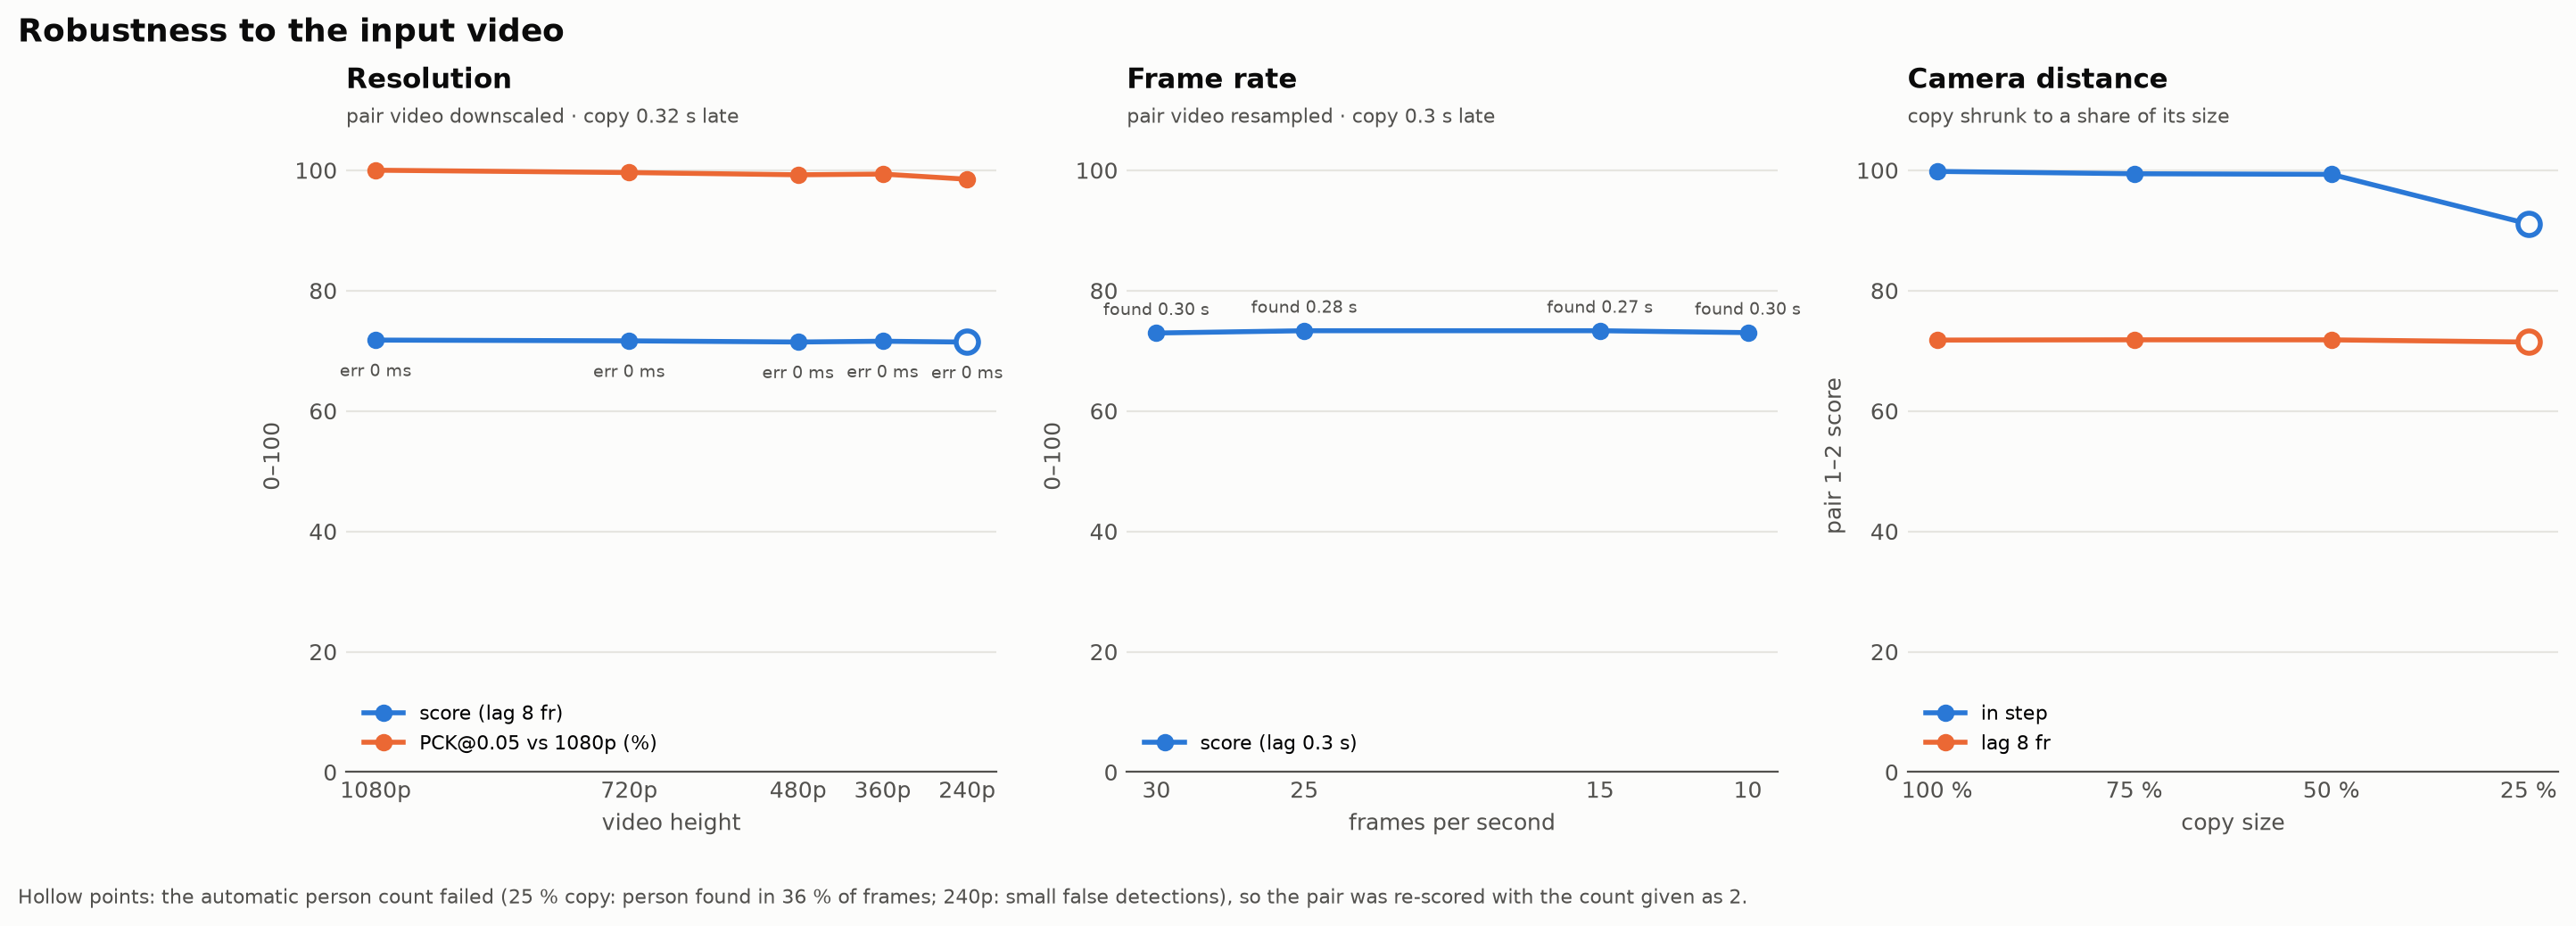
\includegraphics[width=\linewidth]{fig13_robustness}
\caption{Нягтаршил, кадрын давтамж болон камерын зайн нөлөө}
\label{fig:fig13_robustness}
\end{figure}

Хуулбарыг 50\% хүртэл жижигрүүлэхэд оноо 99.8-аас 99.3 болж бараг өөрчлөгдөөгүй нь үений өнцөгт суурилсан арга хүний зураг дээрх хэмжээнээс хамааралгүй болохыг баталж байна. Нягтаршлыг 1080p-ээс 360p хүртэл бууруулахад гол цэгийн 99.2\%-иас дээш нь жишиг байрлалынхаа хүрээний өндрийн 5\%-ийн дотор үлдэж, оноо 71.5--71.8, хоцрогдлын алдаа 0 мс байв. Кадрын давтамжийг 10 кадр/с хүртэл бууруулахад хоцрогдлын алдаа 0--33 мс буюу тухайн давтамжийн нэг кадрын хугацаанаас (33--100 мс) бага байсан бөгөөд оноо 73.0--73.3 хооронд тогтвортой байв.

Хоёр тохиолдолд хүний тоог автоматаар тодорхойлох алхам алдаа гаргасан (Хүснэгт~\ref{tab:robustness}-ийн * тэмдэгтэй мөрүүд). Хуулбарыг 25\% хүртэл жижигрүүлэхэд (хүний өндөр ойролцоогоор 140 пиксел) хүн илрүүлэгч жижиг хүнийг кадруудын ердөө 36\%-д илрүүлсэн тул эхний 2 секундэд хамгийн олон давтагдсан илрүүлэлтийн тоо 1 болж, хос үүсээгүй. 240p нягтаршилд жижиг, итгэлцэл багатай худал илрүүлэлтүүд олон гарч хүний тоо 4 гэж тоологдсон. Хүний тоог 2 гэж гараар өгөхөд хоёр тохиолдолд хоцрогдол зөв олдож, оноо нь бусад нөхцөлтэй ойролцоо гарсан. Харин 25\%-ийн синхрон бичлэгийн оноо (91.1) бусдаас бага байгаа нь 2-р хүн кадруудын 64\%-д илрээгүй, нөхөгдөх боломжгүй урт завсар үүссэнтэй холбоотой. Иймд хүний өндөр 140 пикселээс бага эсвэл бичлэгийн нягтаршил 240p-ээс бага үед системийг найдвартай гэж үзэхгүй бөгөөд хэрэглэгч хүний тоог гараар өгөх боломжтой байх нь зүйтэй.

\textbf{Хүний тоо.} Эх бичлэгийн 2, 3, 4 хуулбарыг зэрэгцүүлж, сүүлийн хуулбарыг 8 кадраар хоцроосон бичлэгүүд дээр хоцорсон хүнийг бүх тохиолдолд хамгийн бага оноотой (\(S_i\) нь 71.6--71.8, бусад хүмүүсийнх 85.7--90.4) гэж зөв илрүүлсэн (Зураг~\ref{fig:fig14_people}). Синхрон хүмүүсийн хоорондох хосын оноо 99.7--99.8 байсан тул хүний тоо нэмэгдэхэд бүлгийн оноо 71.8, 81.1, 85.7 болж өссөн нь нэг хүний зөрүү олон хосын дунджид шингэж байгааг харуулна. Иймд олон хүнтэй бичлэгт бүлгийн онооноос гадна хүн тус бүрийн оноог харах шаардлагатай. Нэг кадрын боловсруулалтын хугацаа хүн бүрт дунджаар 17 мс нэмэгдэж, 2, 3, 4 хүнд 58, 74, 91 мс болсон нь дээрээс доош загварын хүлээгдэж буй шинж юм.

\begin{figure}[H]
\centering
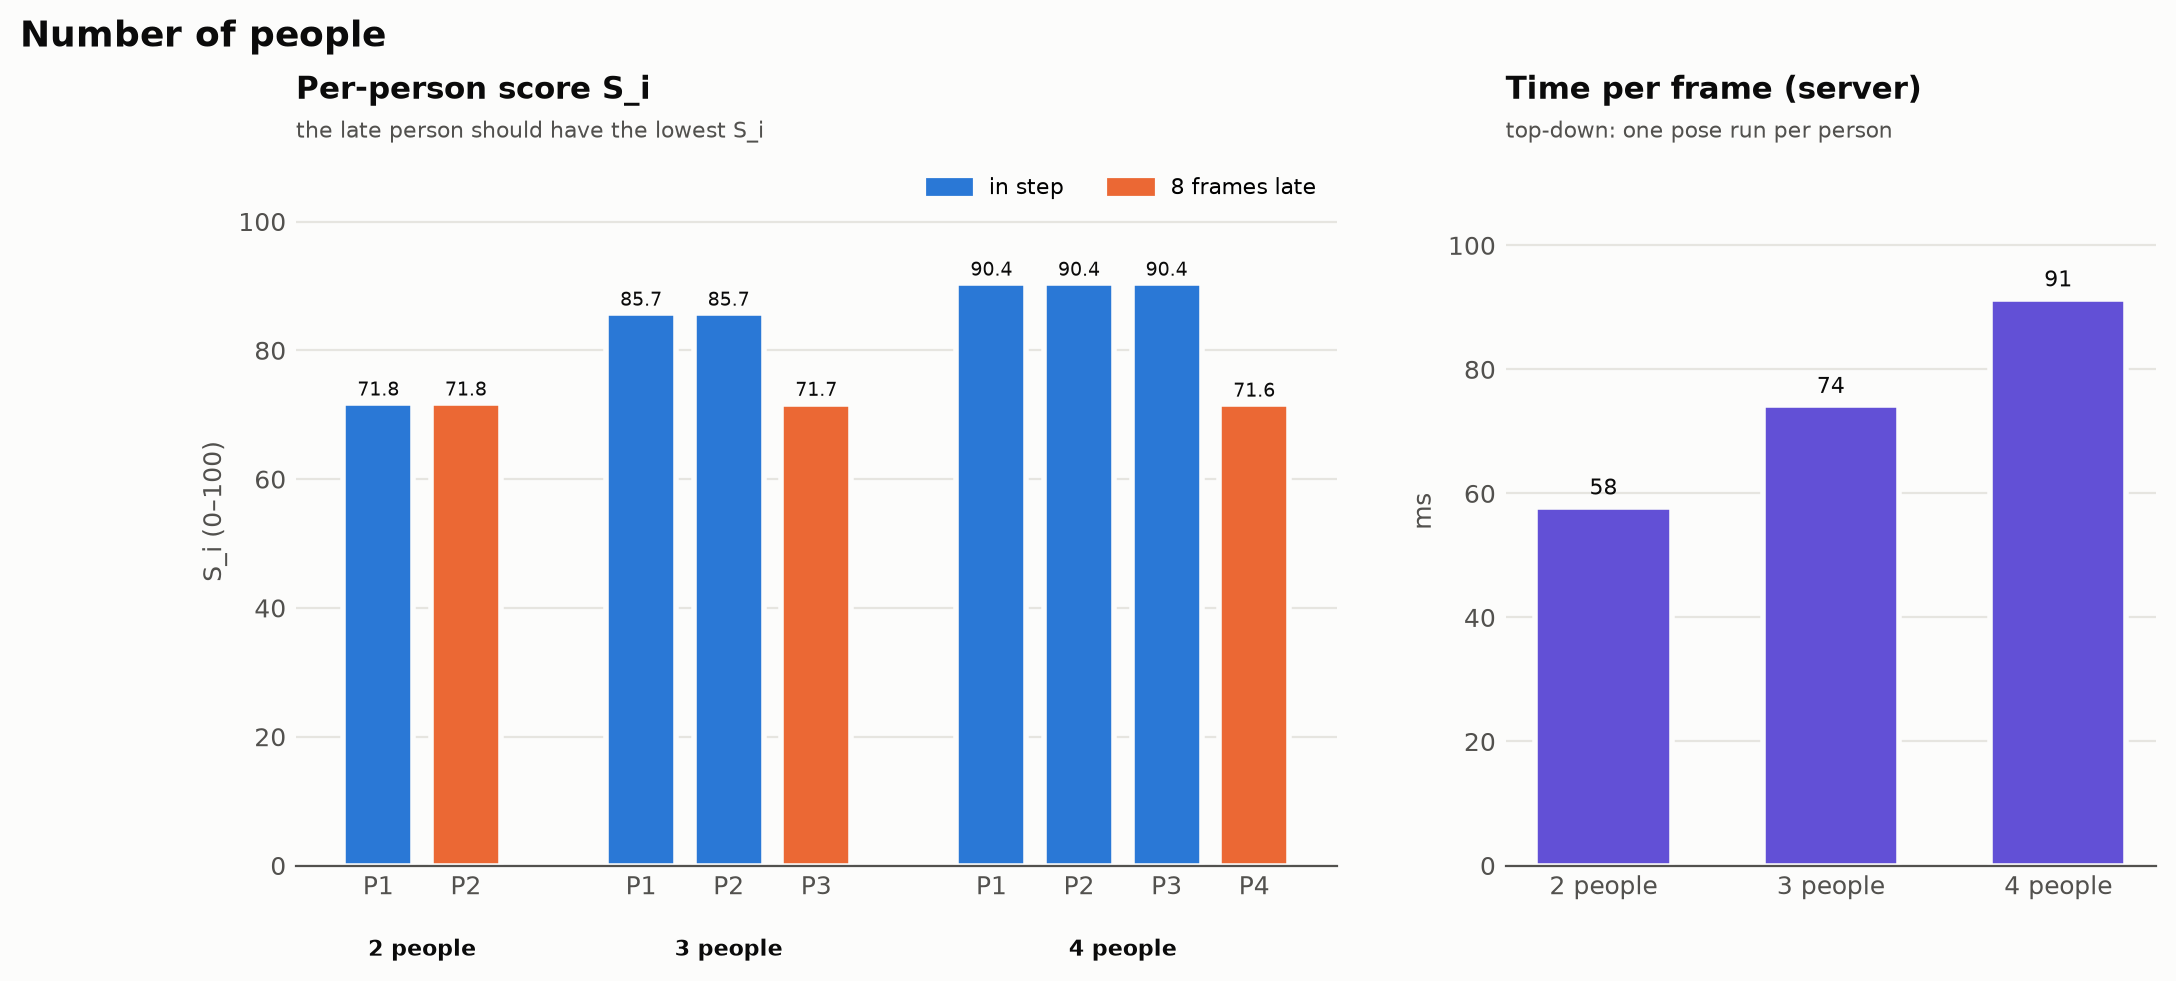
\includegraphics[width=\linewidth]{fig14_people}
\caption{Хүний тооноос хамаарах хүн тус бүрийн оноо болон нэг кадрын хугацаа}
\label{fig:fig14_people}
\end{figure}

\textbf{Шуугиан тэгшитгэлийн нөлөө.} Хүний тоо автоматаар зөв тоологдсон 30 хяналттай бичлэгийн оноог Савицкий-Голейн тэгшитгэлтэй болон тэгшитгэлгүйгээр тооцоолж харьцуулахад оноо дунджаар 0.59, хамгийн ихдээ 4.3 оноогоор зөрсөн. Тэгшитгэлгүй үед синхрон бичлэгүүдийн оноо 0.4--0.8 оноогоор буурсан бол өөр хөдөлгөөнтэй бичлэгүүдийнх 2.9--4.3 оноогоор буурсан бөгөөд хоцрогдлын үр дүн өөрчлөгдөөгүй. Энэхүү өндөр нягтаршилтай, тод бичлэгт гол цэгийн чичиргээ бага тул тэгшитгэлийн нөлөө бага гарсан. Чичиргээ ихтэй бичлэгт нөлөө нь илүү их байх төлөвтэй.

\textbf{Хоцрогдол оруулсан гол цэгийн түвшний туршилт.} Синхрончлол алдагдсан мөчийг хоцорсон хүн болон биеийн хэсгийн хамт зөв илрүүлж байгаа эсэхийг гол цэгийн түвшинд шалгав. Загвар сонголтын бичлэгийн нэг хүний бүх бие эсвэл нэг, хоёр мөчийн гол цэгийг 2.5--3 секундийн турш 0.3 эсвэл 0.5 секундээр хоцроож (t кадрын гол цэгийг тухайн хүний t − Δ кадрын гол цэгээр сольж), хоёр өөр хүн, хоёр өөр хугацаанд нийт 20 тохиолдол үүсгэв. Тохиолдол бүрт хоцроосон хугацаатай давхцсан, тухайн хүнийг агуулсан шинэ мөч илэрсэн, хоцорсон хүн болон мөчийг зөв нэрлэсэн эсэхийг шалгав (Хүснэгт~\ref{tab:delay_test}).

\begin{table}[H]
\centering
\caption{Хоцрогдол оруулсан гол цэгийн түвшний туршилтын үр дүн}
\label{tab:delay_test}
\small
\begin{tabular}{|>{\raggedright\arraybackslash}p{0.220\linewidth}|>{\raggedright\arraybackslash}p{0.140\linewidth}|>{\raggedright\arraybackslash}p{0.220\linewidth}|>{\raggedright\arraybackslash}p{0.280\linewidth}|}
\hline
\textbf{Хоцроосон хэсэг} & \textbf{Хоцрогдол} & \textbf{Зөв илрүүлсэн} & \textbf{Олдсон хоцрогдол (с)} \\ \hline
Бүх бие & 0.3 с & 2/2 & 0.48, 0.52 \\ \hline
Бүх бие & 0.5 с & 2/2 & 0.56, 0.68 \\ \hline
Хоёр гар & 0.3 с & 2/2 & 0.52, 1.08 \\ \hline
Хоёр гар & 0.5 с & 2/2 & 0.92, 1.32 \\ \hline
Баруун гар & 0.3 с & 2/2 & 0.68, 0.40 \\ \hline
Баруун гар & 0.5 с & 2/2 & 0.96, 0.60 \\ \hline
Хоёр хөл & 0.3 с & 2/2 & 0.28, 0.44 \\ \hline
Хоёр хөл & 0.5 с & 2/2 & 0.52, 0.60 \\ \hline
Зүүн хөл & 0.3 с & 0/2 & -- \\ \hline
Зүүн хөл & 0.5 с & 2/2 & 0.52, 0.56 \\ \hline
\textbf{Нийт} & & \textbf{18/20} & \\ \hline
\end{tabular}
\end{table}

20 тохиолдлын 18-д нь хоцорсон хүн болон мөчийг зөв илрүүлсэн бөгөөд илрүүлж чадаагүй хоёр тохиолдол хоёулаа нэг хөлийг 0.3 секундээр хоцроосон тохиолдол байв. Тухайн хугацаанд хөл бага хөдөлсөн үед хоцрогдол өнцгийн зөрүүнд бага нөлөөлдөг тул илрүүлэхэд хэцүү. Харин мөчийн түвшинд олдсон хоцрогдлын утга ихэнхдээ бодит хоцрогдлоос их гарсан (0.3 секундийг 0.28--1.08 секунд гэх мэт). Тулааны урлагийн хөдөлгөөн давтагддаг тул шилжилт нь мөчийг тухайн хөдөлгөөний өөр давталттай тааруулж болдог бөгөөд мөчийн хоцрогдлын хэмжээг тайлбарлахдаа үүнийг анхаарах шаардлагатай. Бүх биеийн хоцрогдлыг бүтэн бичлэгийн хувьд тооцоолоход (дээрх видеоны түвшний туршилт) ийм алдаа гараагүй.

\textbf{Хоцрогдлын онооны тогтворгүй байдал.} Гол цэгүүд бараг ижил (медиан 0.61 пиксел) байхад 4.3-ын хөтөч ба серверийн бүлгийн оноо 1.2 оноогоор, кадр бүрийн оноо 95-р перцентилээр 10.8 оноогоор зөрсөн. Бүрэлдэхүүн бүрээр задлан шинжлэхэд \(S_{pose}\) (медиан зөрүү 0.001) болон \(S_{corr}\) (0.003) бараг ижил байсан бол нийт 2568 цонхны 477-д нь \(S_{lag}\) өөр гарсан. Энэ бичлэгт цонхны \(\rho_{max}\)-ийн дундаж 0.44 буюу \(\rho_{min} = 0.3\) босгод ойрхон тул гол цэгийн өчүүхэн өөрчлөлт \(\rho_{max}\)-ийг босгоос дээш эсвэл доош гаргахад \(S_{lag}\) ойролцоогоор 0.9-өөс 0 руу огцом өөрчлөгддөг. Иймд босгын орчмын гурван хувилбарыг харьцуулав. Үүнд: одоогийн огцом босго (hard), босгын орчимд \(S_{lag}\)-ийг жигд өсгөх налуу (ramp), \(\rho_{max} < \rho_{min}\) үед хоцрогдлыг «хэмжигдээгүй» гэж үзэн онооноос хасах (drop). Налуу хувилбарт

\begin{equation}
S_{lag} = \max\left(0, \; 1 - \frac{|\tau^{*}|}{\tau_{max}}\right) \cdot \min\left(1, \; \max\left(0, \; \frac{\rho_{max} - (\rho_{min} - w/2)}{w}\right)\right)
\end{equation}

бөгөөд \(w = 0.2\) үед \(S_{lag}\) нь \(\rho_{max} = 0.2\)-оос 0.4 хүртэл 0-ээс одоогийн утга хүртэл жигд өснө. Хувилбар бүрийг тогтвортой байдал (ижил бичлэгийн хөтөч ба серверийн ажиллуулалтын онооны зөрүү) болон ялгах чадвар (2-р хүнийг гол цэгийн түвшинд 0.12--0.8 секундээр хоцроох, эсвэл тухайн хүний 7 болон 13 секундийн зайтай өөр хэсгийн хөдөлгөөнөөр солиход 1--2 хосын оноо зөв дарааллаар буурч байгаа эсэх) гэсэн хоёр шалгуураар үнэлэв (Хүснэгт~\ref{tab:lag_variants}, Зураг~\ref{fig:fig9_lag_confidence}).

\begin{table}[H]
\centering
\caption{Хоцрогдлын онооны хувилбаруудын харьцуулалт}
\label{tab:lag_variants}
\small
\begin{tabular}{|>{\raggedright\arraybackslash}p{0.120\linewidth}|>{\raggedright\arraybackslash}p{0.180\linewidth}|>{\raggedright\arraybackslash}p{0.180\linewidth}|>{\raggedright\arraybackslash}p{0.400\linewidth}|}
\hline
\textbf{Хувилбар} & \textbf{Бүлгийн онооны зөрүү} & \textbf{Кадр бүрийн зөрүү (95-р перцентиль)} & \textbf{1--2 хосын оноо: синхрон / 0.12 / 0.2 / 0.4 / 0.8 с хоцрогдол / өөр хөдөлгөөн (7 с, 13 с)} \\ \hline
hard & 1.21 & 10.75 & 82.8 / 77.9 / 73.8 / 65.9 / 54.1 / 48.1, 46.8 \\ \hline
ramp 0.2 & 0.39 & 5.10 & 83.4 / 78.2 / 74.1 / 66.1 / 54.0 / 48.7, 47.5 \\ \hline
ramp 0.4 & 0.11 & 4.43 & 82.1 / 77.2 / 73.2 / 65.4 / 53.6 / 50.3, 50.7 \\ \hline
drop & 0.09 & 2.05 & 88.1 / 82.9 / 78.7 / 70.5 / 63.2 / 66.0, 68.0 \\ \hline
\end{tabular}
\end{table}

\begin{figure}[H]
\centering
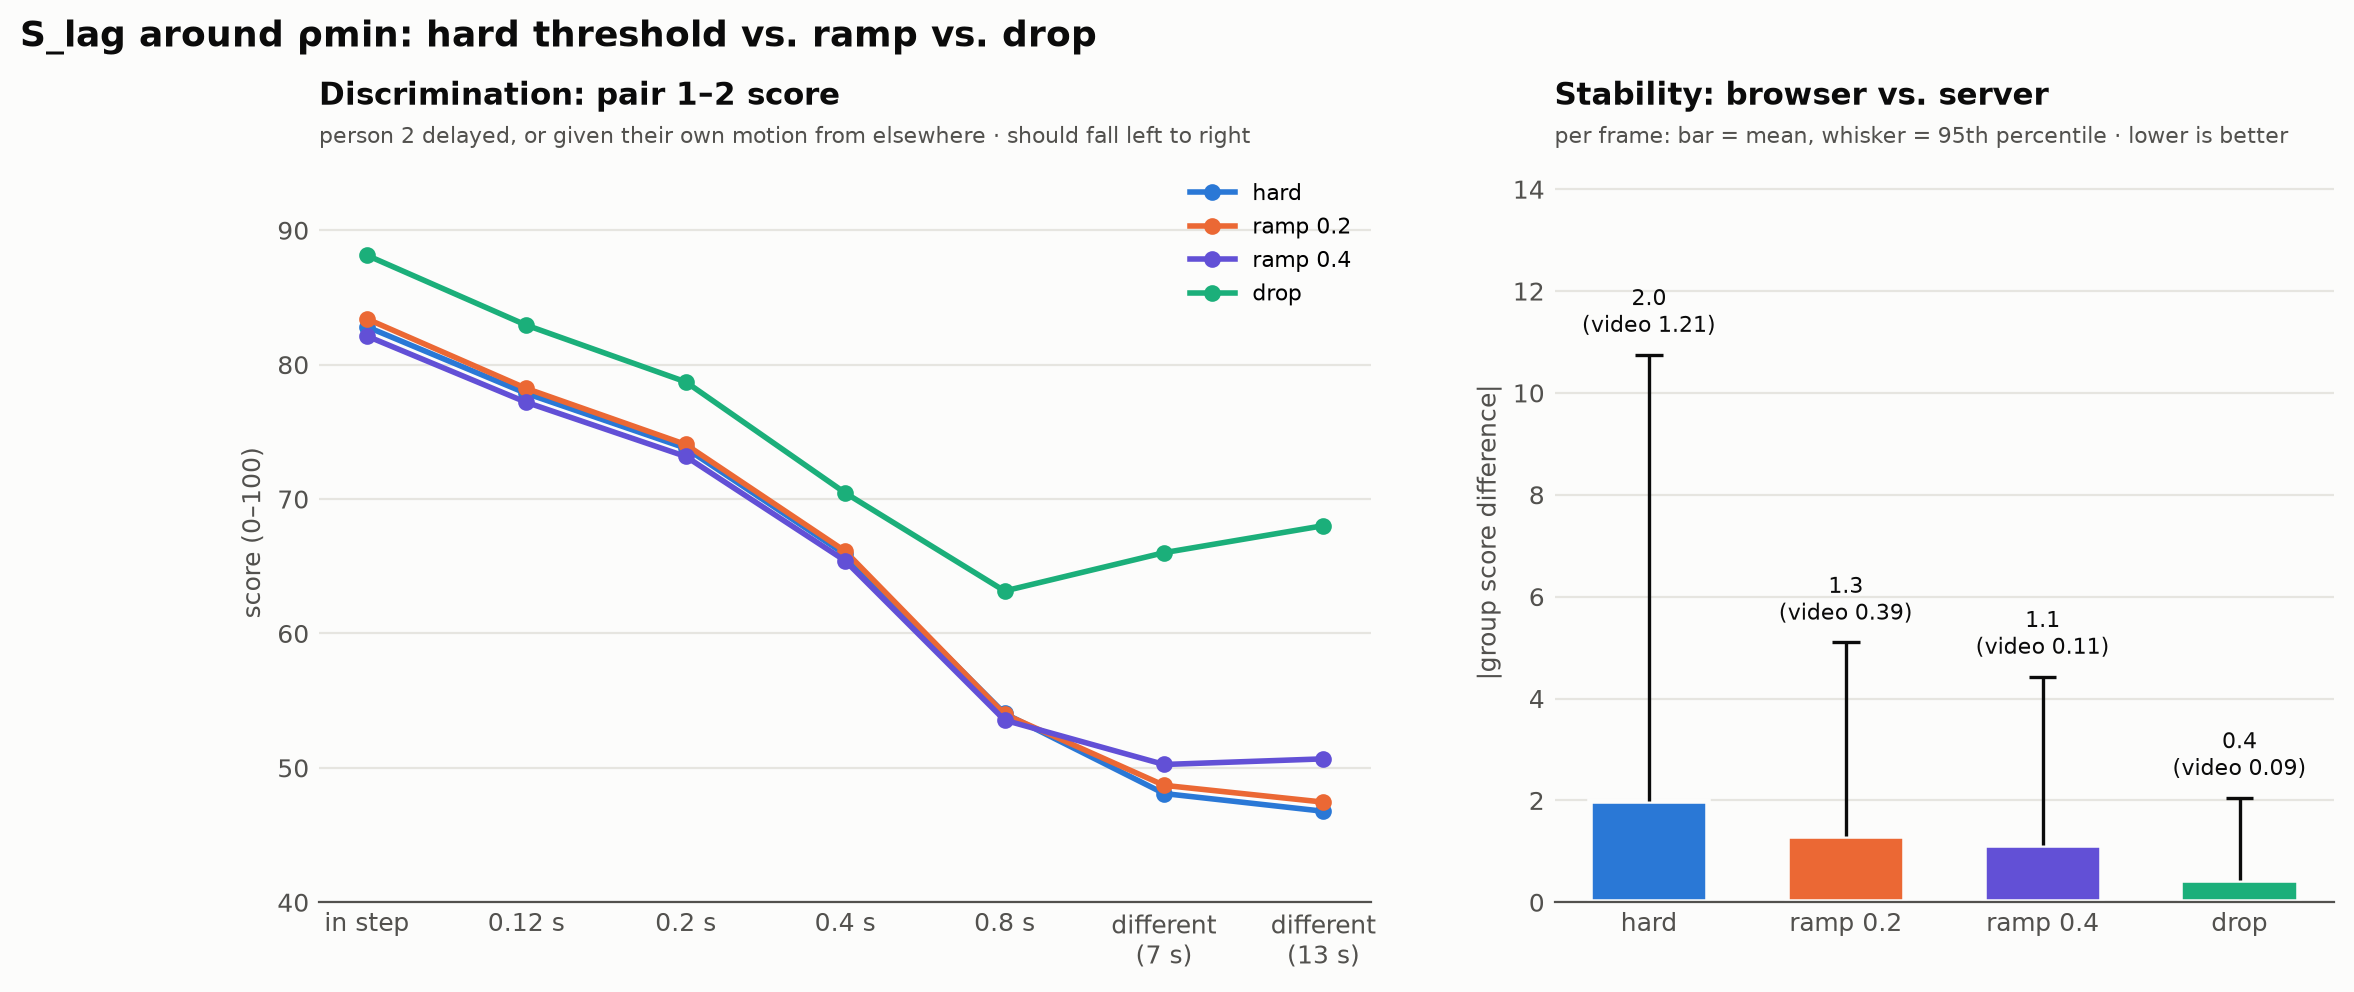
\includegraphics[width=\linewidth]{fig9_lag_confidence}
\caption{Хоцрогдлын онооны хувилбаруудын ялгах чадвар ба тогтвортой байдал}
\label{fig:fig9_lag_confidence}
\end{figure}

Хасах (drop) хувилбар хамгийн тогтвортой боловч өөр хөдөлгөөнд (66--68) 0.8 секундийн хоцрогдлоос (63.2) илүү өндөр оноо өгч байгаа тул ашиглах боломжгүй. Учир нь хоцрогдлыг хэмжих боломжгүй байх нь синхрон бус байгаагийн шинж бөгөөд түүнийг онооноос хасах нь торгуулийг арилгаж байна. Налуу хувилбарын \(w = 0.4\) нь илүү тогтвортой ч \(\rho_{max} \approx 0.1\) буюу бараг хамааралгүй цонхонд ч \(S_{lag}\) өгдөг тул өөр хөдөлгөөний оноо өсч, ялгах чадвар буурсан. Харин \(w = 0.2\) нь бүлгийн онооны зөрүүг 3 дахин (1.21-ээс 0.39), кадр бүрийн зөрүүг 2 дахин бууруулж, ялгах чадвар нь одоогийн хувилбартай бараг ижил хэвээр байна. Мөн түүний муж (0.2--0.4) нь өөр хөдөлгөөний (0.13) болон хамт хөдөлж буй хүмүүсийн (0.42) \(\rho_{max}\)-ийн медиануудын хооронд оршдог. Хүний тоо автоматаар зөв тоологдсон 30 хяналттай бичлэг дээр налуу хувилбарын оноо анхдагч хувилбарынхаас дунджаар 0.11, хамгийн ихдээ 2.4 оноогоор зөрсөн бөгөөд нөхцлүүдийн дараалал өөрчлөгдөөгүй. Иймд \(w = 0.2\) налуу хувилбарыг ашиглахыг санал болгож байна. Энэ бүлгийн бусад бүх үр дүнг анхдагч огцом босгоор (hard) тооцоолсон. Кадр бүрийн онооны үлдсэн зөрүү (95-р перцентиль 5.1) нь хөндлөн корреляцын хоёр ойролцоо оргилын хооронд \(\tau^{*}\) үсрэхээс үүдэлтэй.

\headshort{Бодит бичлэг}
\section{Бодит бичлэг дээрх туршилт}

\textbf{Тулааны урлагийн бичлэг.} Загвар сонголтын бичлэгт гурван хүн тулааны урлагийн ижил хөдөлгөөнийг хамтдаа хийдэг. Синхрончлолын алгоритмаар бүлгийн оноо 82.6 гарав (Хүснэгт~\ref{tab:sync_result}).

\begin{table}[H]
\centering
\caption{Тулааны урлагийн бичлэгийн синхрончлолын үр дүн}
\label{tab:sync_result}
\small
\begin{tabular}{|>{\raggedright\arraybackslash}p{0.130\linewidth}|>{\raggedright\arraybackslash}p{0.090\linewidth}|>{\raggedright\arraybackslash}p{0.090\linewidth}|>{\raggedright\arraybackslash}p{0.090\linewidth}|>{\raggedright\arraybackslash}p{0.090\linewidth}|>{\raggedright\arraybackslash}p{0.180\linewidth}|>{\raggedright\arraybackslash}p{0.120\linewidth}|}
\hline
\textbf{Хос} & \textbf{Оноо} & \textbf{Гар} & \textbf{Хөл} & \textbf{Их бие} & \textbf{Хоцрогдол (\(\rho_{max}\))} & \textbf{Толин тусгал} \\ \hline
1--2 & 83.6 & 81.8 & 90.4 & 86.6 & 0 с (0.31) & 0.4\% \\ \hline
1--3 & 79.5 & 77.3 & 81.7 & 79.9 & 0.08 с (0.23) & 11.6\% \\ \hline
2--3 & 84.6 & 80.8 & 86.1 & 87.0 & 0.04 с (0.28) & 5.8\% \\ \hline
\end{tabular}
\end{table}

Хүн тус бүрийн оноо \(S_1 = 81.6\), \(S_2 = 84.1\), \(S_3 = 82.0\) бөгөөд 1-р хүн бүлгээсээ хамгийн их зөрж байна. Бүх хосод гарын оноо хамгийн бага байгаа нь хурдан хөдөлдөг, чичиргээ ихтэй бугуйн цэгүүдтэй (3.2) уялдана. Бүх бичлэгийн хоцрогдлын хувьд 1--3 болон 2--3 хосын \(\rho_{max}\) нь \(\rho_{min} = 0.3\)-аас бага тул тэдгээрт итгэхгүй. Кадр бүрийн онооны графикаас (Зураг~\ref{fig:fig8_sync_timeline}) бичлэгийн эхний 20 секундэд бүлгийн оноо ихэвчлэн 85--93 байхад 20-оос хойш хэд хэдэн удаа 60--66 хүртэл буурч байгааг харж болно. Алгоритм нийт 12 синхрончлол алдагдсан мөч илрүүлсэн бөгөөд тэдгээрийн ихэнх нь гарын хоцрогдол байв.

\begin{figure}[H]
\centering
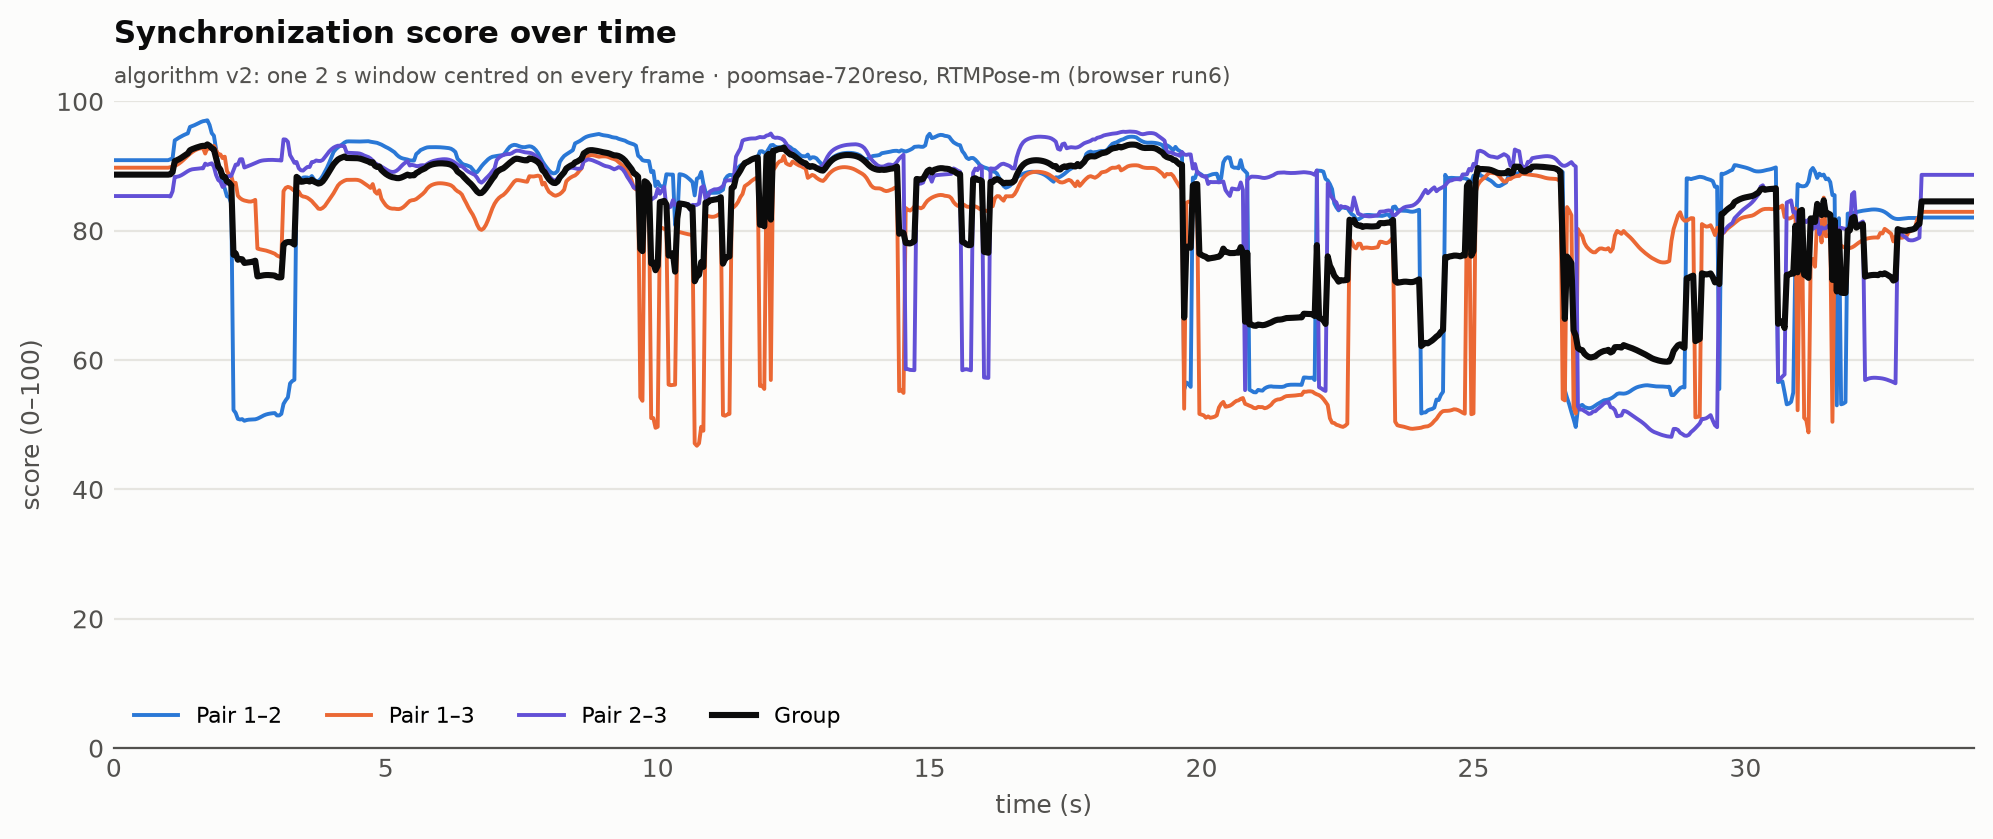
\includegraphics[width=\linewidth]{fig8_sync_timeline}
\caption{Бүлгийн болон хос бүрийн синхрончлолын оноо (кадр бүрээр)}
\label{fig:fig8_sync_timeline}
\end{figure}

\textbf{Бүжгийн бичлэгүүд.} Гурван бүжигчин ижил бүжгийг хамтдаа бүжиглэсэн дөрвөн бичлэгийн үр дүнг Хүснэгт~\ref{tab:real}-д нэгтгэв.

\begin{table}[H]
\centering
\caption{Гурван хүнтэй бүжгийн бичлэгүүдийн синхрончлолын үр дүн}
\label{tab:real}
\small
\begin{tabular}{|>{\raggedright\arraybackslash}p{0.100\linewidth}|>{\raggedright\arraybackslash}p{0.090\linewidth}|>{\raggedright\arraybackslash}p{0.140\linewidth}|>{\raggedright\arraybackslash}p{0.090\linewidth}|>{\raggedright\arraybackslash}p{0.190\linewidth}|>{\raggedright\arraybackslash}p{0.110\linewidth}|>{\raggedright\arraybackslash}p{0.090\linewidth}|}
\hline
\textbf{Бичлэг} & \textbf{Урт (с)} & \textbf{Гурван хүн илэрсэн кадр} & \textbf{Бүлгийн оноо} & \textbf{\(S_1 / S_2 / S_3\)} & \textbf{Нэг кадрын хугацаа (мс)} & \textbf{Зөрсөн мөч} \\ \hline
1 & 42.6 & 93.1\% & 69.4 & 68.1 / 71.2 / 68.8 & 71.6 & 15 \\ \hline
2 & 42.6 & 86.0\% & 67.0 & 67.5 / 67.7 / 65.7 & 70.6 & 16 \\ \hline
3 & 34.9 & 86.4\% & 71.2 & 71.6 / 71.8 / 70.2 & 62.3 & 13 \\ \hline
4 & 30.7 & 98.3\% & 79.1 & 80.6 / 77.0 / 79.8 & 72.0 & 9 \\ \hline
\end{tabular}
\end{table}

Бодит бүжигчдийн бүлгийн оноо 67.0--79.1 буюу нэг хүний хуулбартай синхрон бичлэгийнхээс (99.8) мэдэгдэхүйц бага, харин өөр хөдөлгөөний онооноос (45.4--62.0) их гарсан. Энэ нь ижил бүжгийг хамтдаа бүжиглэсэн ч хүмүүсийн хөдөлгөөний далайц, хэлбэр, хэмнэлд байгалийн зөрүү байдагтай нийцнэ. Бичлэгүүдийн бүх бичлэгийн \(\rho_{max}\) 0.13--0.35 хооронд байсан бөгөөд ихэнх хосод \(\rho_{min} = 0.3\)-аас бага тул бүх бичлэгийн хоцрогдлыг найдвартай гэж үзээгүй. Бүжигчид бие биеийнхээ урдуур, хойгуур шилжиж халхалдаг тул гурван хүн бүгд илэрсэн кадрын хувь 86.0--98.3\% байсан ба дутуу кадруудыг 3.4-ийн аргаар нөхсөн. Хамгийн өндөр оноотой 4-р бичлэгт хосуудын хөлийн оноо 85.3--88.9 байхад гарын оноо 62.8--76.1 байсан нь бүжигчдийн гарын хөдөлгөөн хөлийнхөөс илүү зөрж байгааг харуулна. Бүжигчдийн синхрончлолын жинхэнэ түвшин тэмдэглэгдээгүй тул эдгээр оноо зөв эсэхийг шүүгчийн үнэлгээтэй харьцуулж баталгаажуулах шаардлагатай.

\textbf{Загвар бүрийн нягтаршлын нөлөө.} Загвар сонголтын шатанд тулааны урлагийн бичлэгийг 360p, 480p, 720p нягтаршилтай хувилбараар таван загвараар боловсруулж, 720p-ийн үр дүнтэй харьцуулсан (Зураг~\ref{fig:fig10_resolution}). RTMPose-m бүх нягтаршилд кадрын 100\%-д гурван хүнийг бүгдийг нь илрүүлж, 720p-ийн гол цэгээс хүрээний өндрийн 5\%-ийн дотор байсан гол цэгийн хувь 480p-д 98.6\%, 360p-д 94.5\% байв. MediaPipe-ийн хувьд 68\% ба 75\% байсан нь нягтаршилд хамгийн мэдрэмтгий байв. Энэ туршилтыг кадр унших алдааг засахаас өмнө 30 кадр/с давтамжаар хийсэн боловч хяналттай бичлэг дээрх нягтаршлын туршилт (4.4) нь RTMPose-m-ийн хувьд ижил дүгнэлтэд хүрсэн.

\begin{figure}[H]
\centering
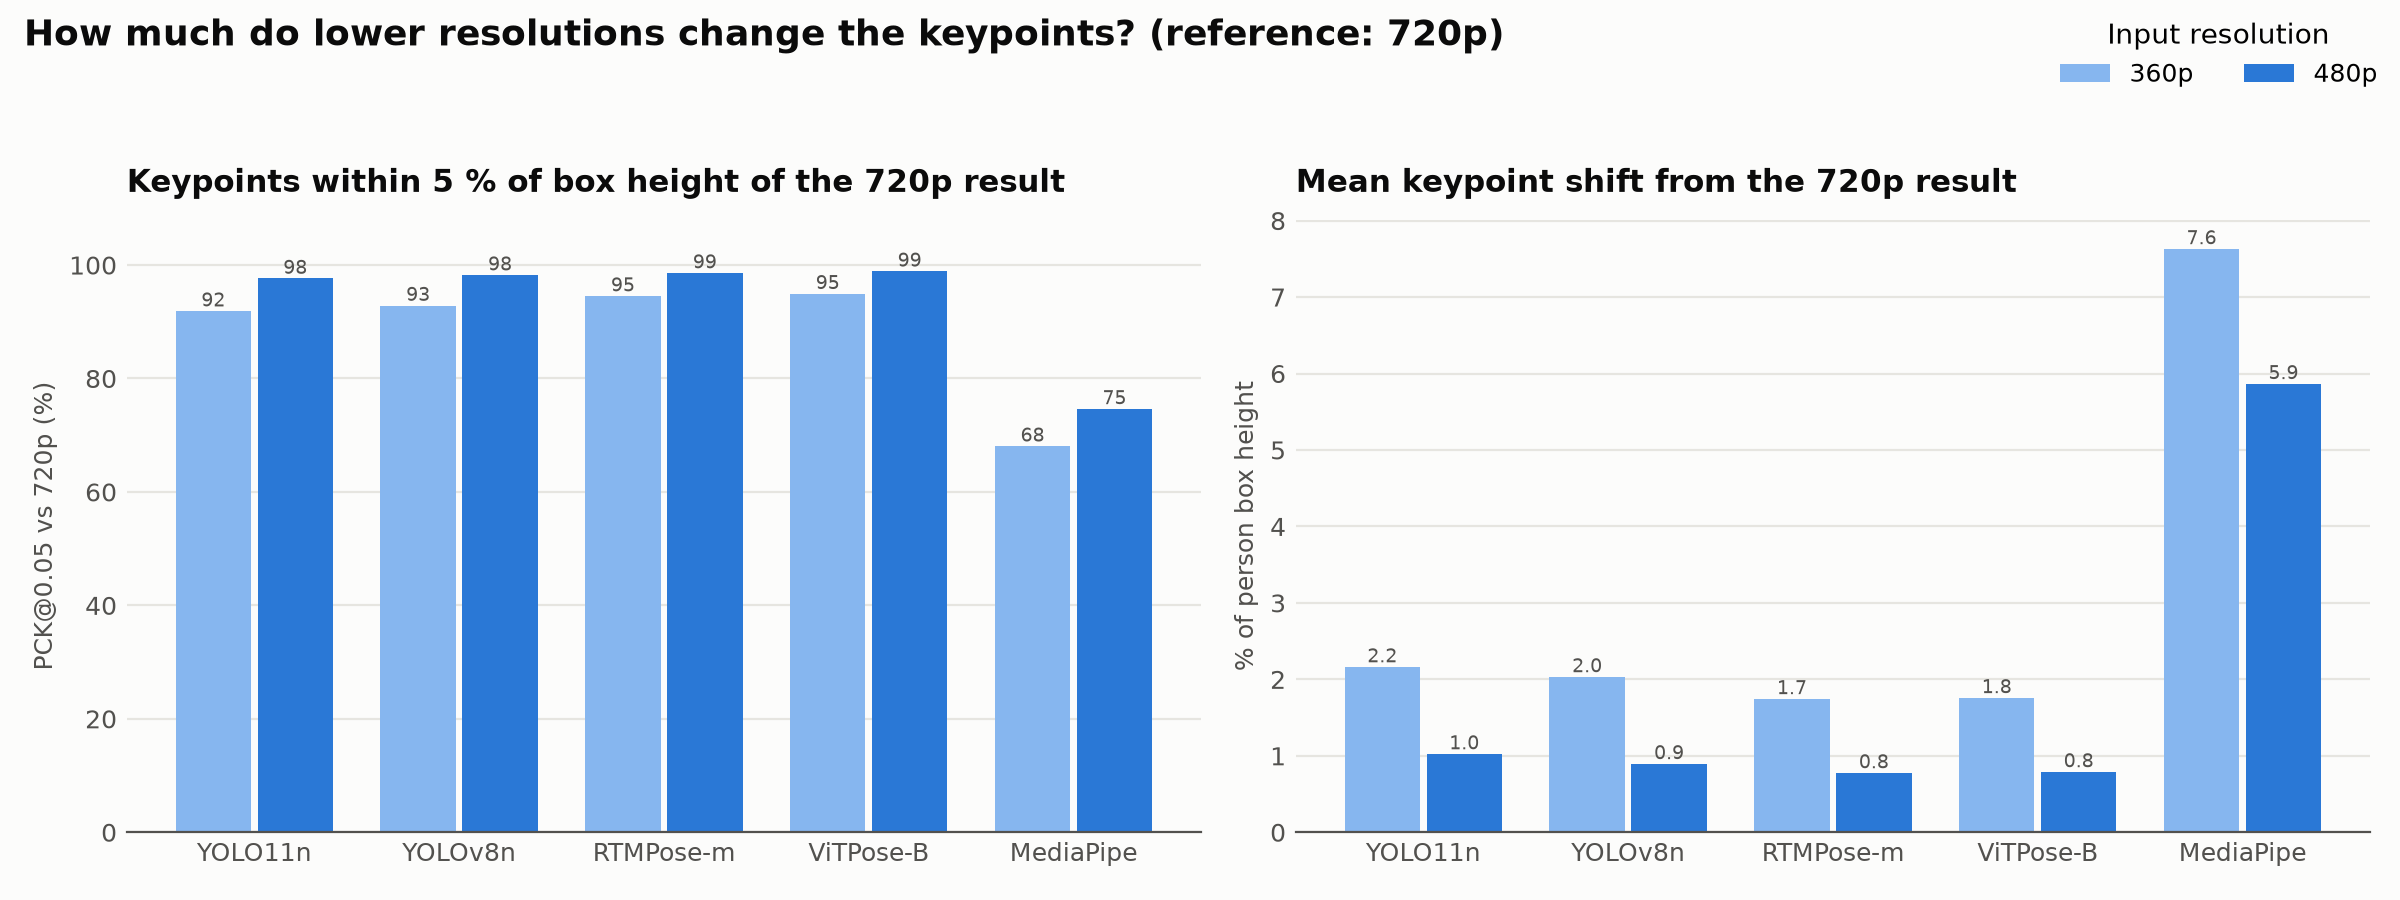
\includegraphics[width=\linewidth]{fig10_resolution}
\caption{Бага нягтаршилд гол цэгийн 720p-ийн үр дүнтэй тохирох байдал ба дундаж шилжилт}
\label{fig:fig10_resolution}
\end{figure}

\section{Аргын хязгаарлалт}

Туршилтын үр дүнд үндэслэн аргын дараах хязгаарлалтыг тодорхойлов. Үүнд:

\begin{itemize}
\item
  Хүний тоог эхний 2 секундийн илрүүлэлтээр автоматаар тодорхойлдог тул хүний өндөр ойролцоогоор 140 пикселээс бага эсвэл бичлэгийн нягтаршил 240p ба түүнээс бага үед хүний тоо буруу тоологдож болно. Энэ үед хэрэглэгч хүний тоог гараар өгөх шаардлагатай.
\item
  Ойролцоогоор 1 секунд ба түүнээс их хоцрогдол оноогоороо өөр хөдөлгөөнтэй ижил түвшинд хүрдэг тул тэдгээрийг ялгахдаа бүх бичлэгийн хоцрогдол ба \(\rho_{max}\)-ийг хамт харах шаардлагатай.
\item
  Мөчийн түвшний хоцрогдлын хэмжээ давтагддаг хөдөлгөөнд бодит утгаасаа их гарч болох бөгөөд бага хөдөлж буй мөчийн (жишээлбэл, 0.3 секундийн хөлийн) хоцрогдлыг илрүүлэх боломжгүй.
\item
  Хоцрогдлын оноо \(\rho_{min}\) босгын орчимд огцом өөрчлөгддөг тул гол цэгийн өчүүхэн ялгаа кадр бүрийн оноонд мэдэгдэхүйц нөлөөлдөг. Налуу хувилбар энэ нөлөөг бууруулна.
\item
  Үений өнцгийг 2D зураг дээр тооцоолдог тул хүмүүс камерт ойролцоо ижил чиглэлээр харсан байх шаардлагатай. Мөн хүмүүс байраа солихгүй, бие биеэ удаан хугацаанд бүрэн халхлахгүй гэж үзсэн.
\item
  Хяналттай өгөгдөл нь нэг хүний бичлэгийн хуулбар тул бодит хүмүүсийн хооронд байдаг хөдөлгөөний байгалийн зөрүү, биеийн хэмжээ, хувцасны ялгааг агуулаагүй. Бодит бичлэгүүдийн синхрончлолын жинхэнэ түвшин тэмдэглэгдээгүй тул бодит бичлэг дээрх үр дүнг шүүгчийн үнэлгээтэй харьцуулаагүй.
\item
  Биеийн хэсгийн жин болон нэгдсэн онооны жингүүдийг (\(w_1 = w_2 = w_3\)) судлаач тогтоосон бөгөөд өгөгдөлд суурилан тохируулаагүй.
\end{itemize}


%----------------------------------------------------------------------------------------
%   Дүгнэлт
%----------------------------------------------------------------------------------------
\conclusion{Дүгнэлт}
Энэхүү судалгааны ажлын хүрээнд хоёр болон түүнээс дээш хүний хөдөлгөөнийг агуулсан видео бичлэгээс хүний биеийн гол цэгүүдийг тодорхойлж, тэдгээрийн хөдөлгөөний синхрончлолыг 0--100 хуваарьт тоон утгаар үнэлэх систем боловсруулж, хяналттай болон бодит бичлэгүүд дээр туршсан. Судалгааны зорилтуудын хүрээнд дараах үр дүнд хүрэв.

\begin{enumerate}
\def\labelenumi{\arabic{enumi}.}
\item
  Хүний байрлал тодорхойлох технологи, гол цэгийн форматууд болон хөдөлгөөний ижил төстэй байдлыг хэмжих аргуудыг судалж, үений өнцөгт суурилсан, хүний байрлал ба хэмжээнээс хамааралгүй дүрслэлийг сонгосон (Бүлэг 2).
\item
  Таван HPE загварыг ижил бичлэг дээр илрүүлэлт, гол цэгийн тохирол, чичиргээ, мөчдийн тогтвортой байдал, хурдаар харьцуулж, олон хүнийг тогтвортой илрүүлж, гол цэгийн чанараар хамгийн сайн үр дүн үзүүлсэн RTMPose-m загварыг сонгосон (3.2).
\item
  Хяналттай өгөгдлийг FFmpeg ашиглан нэг хүний бичлэгээс автоматаар үүсгэх арга боловсруулж, хоцрогдол, толин тусгал, өөр хөдөлгөөн, камерын зай, нягтаршил, кадрын давтамж, хүний тооны нийт 32 бичлэг үүсгэсэн (4.1).
\item
  Хүн хуваарилалт, дутуу цэгийг нөхөх, Савицкий-Голейн шүүлтүүрээр тэгшитгэх урьдчилсан боловсруулалтыг хэрэгжүүлсэн (3.3, 3.4).
\item
  Үений өнцгийн зөрүү, Пирсоны корреляц, хөндлөн корреляцаар олсон хоцрогдлыг нэгтгэсэн, кадр бүрийн цонх, биеийн хэсгийн жин, толин тусгал горим бүхий синхрончлолын алгоритм болон синхрончлол алдагдсан мөч, хоцорсон хүн, мөчийг илрүүлэх аргыг боловсруулсан (3.5, 3.6). Системийг вэб хөтөч дээр болон Python сервер дээр ажиллах хоёр горимтойгоор хэрэгжүүлсэн (3.7).
\item
  Видеоны түвшний хяналттай туршилтад алгоритм 0--1 секундийн бүх хоцрогдлыг 0 мс алдаатай олсон, оноо нь хоцрогдол нэмэгдэх тусам 99.8-аас 54.3 хүртэл жигд буурсан, нөхцлүүдийг синхрон \(>\) хоцрогдолтой \(>\) өөр хөдөлгөөн гэсэн дарааллаар ялгасан. Толин тусгал хөдөлгөөнийг 99.3 оноогоор зөв таньж, 3 ба 4 хүнтэй бичлэгт хоцорсон хүнийг зөв илрүүлсэн. Гол цэгийн түвшинд хоцроосон 20 тохиолдлын 18-д хоцорсон хүн болон мөчийг зөв тодорхойлсон. Сервер вэб хөтчөөс 2.2 дахин хурдан ажиллаж, хоёр горимын гол цэг медианаар 0.61 пиксел зөрүүтэй байв (4.3--4.5).
\item
  Хүний хэмжээг 50\%, нягтаршлыг 360p, кадрын давтамжийг 10 кадр/с хүртэл бууруулахад оноо болон хоцрогдлын үр дүн бараг өөрчлөгдөөгүй бол хүний өндөр ойролцоогоор 140 пикселээс, нягтаршил 240p-ээс бага үед хүний тоог автоматаар тодорхойлох алхам алдаа гаргасныг тогтоож, аргын боломж ба хязгаарлалтыг тодорхойлсон (4.4, 4.6).
\end{enumerate}

Мөн судалгааны явцад вэб хөтөч видеог кадрын хил дээр шилжүүлэхэд кадр давхардах, алгасагдах алдааг илрүүлж засварласан бөгөөд хоцрогдлын оноо \(\rho_{min}\) босгын орчимд тогтворгүй болохыг тогтоож, тогтворжуулах налуу хувилбарыг санал болгосон.

Иймд боловсруулсан систем нь энгийн нэг камераар авсан бичлэгээс олон хүний хөдөлгөөний синхрончлолыг тоон, давтагдах боломжтой хэлбэрээр үнэлж, хэн, хэзээ, биеийн аль хэсгээрээ хэр хэмжээгээр зөрж байгааг тодорхойлох боломжтой гэж дүгнэв.


%----------------------------------------------------------------------------------------
%   Ном зүй
%----------------------------------------------------------------------------------------
\singlespace
\addcontentsline{toc}{part}{НОМ ЗҮЙ}
\begin{thebibliography}{99}
	\bibitem{cao2017}
	Cao Z., Simon T., Wei S.-E., Sheikh Y. Realtime Multi-Person 2D Pose Estimation using Part Affinity Fields. CVPR, 2017.
	\bibitem{sun2019}
	Sun K., Xiao B., Liu D., Wang J. Deep High-Resolution Representation Learning for Human Pose Estimation. CVPR, 2019.
	\bibitem{bazarevsky2020}
	Bazarevsky V., Grishchenko I., Raveendran K., Zhu T., Zhang F., Grundmann M. BlazePose: On-device Real-time Body Pose Tracking. arXiv:2006.10204, 2020.
	\bibitem{maji2022}
	Maji D., Nagori S., Mathew M., Poddar D. YOLO-Pose: Enhancing YOLO for Multi Person Pose Estimation Using Object Keypoint Similarity Loss. CVPR Workshops, 2022.
	\bibitem{jiang2023}
	Jiang T., Lu P., Zhang L., Ma N., Han R., Lyu C., Li Y., Chen K. RTMPose: Real-Time Multi-Person Pose Estimation based on MMPose. arXiv:2303.07399, 2023.
	\bibitem{lin2014}
	Lin T.-Y. et al. Microsoft COCO: Common Objects in Context. ECCV, 2014.
	\bibitem{andriluka2014}
	Andriluka M., Pishchulin L., Gehler P., Schiele B. 2D Human Pose Estimation: New Benchmark and State of the Art Analysis. CVPR, 2014.
	\bibitem{jin2020}
	Jin S. et al. Whole-Body Human Pose Estimation in the Wild. ECCV, 2020.
	\bibitem{sakoe1978}
	Sakoe H., Chiba S. Dynamic Programming Algorithm Optimization for Spoken Word Recognition. IEEE Transactions on ASSP, 26(1), 1978.
	\bibitem{savitzky1964}
	Savitzky A., Golay M. J. E. Smoothing and Differentiation of Data by Simplified Least Squares Procedures. Analytical Chemistry, 36(8), 1964.
	\bibitem{xu2022}
	Xu Y., Zhang J., Zhang Q., Tao D. ViTPose: Simple Vision Transformer Baselines for Human Pose Estimation. NeurIPS, 2022.
	\bibitem{ultralytics}
	Jocher G., Chaurasia A., Qiu J. Ultralytics YOLOv8, 2023. \url{https://github.com/ultralytics/ultralytics}
	\bibitem{onnxruntime}
	ONNX Runtime developers. ONNX Runtime. \url{https://onnxruntime.ai}
	\bibitem{fastapi}
	Ramírez S. FastAPI. \url{https://fastapi.tiangolo.com}
	\bibitem{opencv}
	Bradski G. The OpenCV Library. Dr. Dobb's Journal of Software Tools, 2000.
\end{thebibliography}


\end{document}
